\documentclass[twoside]{book}

% Packages required by doxygen
\usepackage{fixltx2e}
\usepackage{calc}
\usepackage{doxygen}
\usepackage{graphicx}
\usepackage[utf8]{inputenc}
\usepackage{makeidx}
\usepackage{multicol}
\usepackage{multirow}
\PassOptionsToPackage{warn}{textcomp}
\usepackage{textcomp}
\usepackage[nointegrals]{wasysym}

% Font selection
\usepackage[T1]{fontenc}
\usepackage[scaled=.90]{helvet}
\usepackage{courier}
\usepackage{amssymb}
\usepackage{sectsty}
\renewcommand{\familydefault}{\sfdefault}
\allsectionsfont{%
  \fontseries{bc}\selectfont%
  \color{darkgray}%
}
\renewcommand{\DoxyLabelFont}{%
  \fontseries{bc}\selectfont%
  \color{darkgray}%
}
\newcommand{\+}{\discretionary{\mbox{\scriptsize$\hookleftarrow$}}{}{}}

% Page & text layout
\usepackage{geometry}
\geometry{%
  a4paper,%
  top=2.5cm,%
  bottom=2.5cm,%
  left=2.5cm,%
  right=2.5cm%
}
\tolerance=750
\hfuzz=15pt
\hbadness=750
\setlength{\emergencystretch}{15pt}
\setlength{\parindent}{0cm}
\setlength{\parskip}{3ex plus 2ex minus 2ex}
\makeatletter
\renewcommand{\paragraph}{%
  \@startsection{paragraph}{4}{0ex}{-1.0ex}{1.0ex}{%
    \normalfont\normalsize\bfseries\SS@parafont%
  }%
}
\renewcommand{\subparagraph}{%
  \@startsection{subparagraph}{5}{0ex}{-1.0ex}{1.0ex}{%
    \normalfont\normalsize\bfseries\SS@subparafont%
  }%
}
\makeatother

% Headers & footers
\usepackage{fancyhdr}
\pagestyle{fancyplain}
\fancyhead[LE]{\fancyplain{}{\bfseries\thepage}}
\fancyhead[CE]{\fancyplain{}{}}
\fancyhead[RE]{\fancyplain{}{\bfseries\leftmark}}
\fancyhead[LO]{\fancyplain{}{\bfseries\rightmark}}
\fancyhead[CO]{\fancyplain{}{}}
\fancyhead[RO]{\fancyplain{}{\bfseries\thepage}}
\fancyfoot[LE]{\fancyplain{}{}}
\fancyfoot[CE]{\fancyplain{}{}}
\fancyfoot[RE]{\fancyplain{}{\bfseries\scriptsize Generated by Doxygen }}
\fancyfoot[LO]{\fancyplain{}{\bfseries\scriptsize Generated by Doxygen }}
\fancyfoot[CO]{\fancyplain{}{}}
\fancyfoot[RO]{\fancyplain{}{}}
\renewcommand{\footrulewidth}{0.4pt}
\renewcommand{\chaptermark}[1]{%
  \markboth{#1}{}%
}
\renewcommand{\sectionmark}[1]{%
  \markright{\thesection\ #1}%
}

% Indices & bibliography
\usepackage{natbib}
\usepackage[titles]{tocloft}
\setcounter{tocdepth}{3}
\setcounter{secnumdepth}{5}
\makeindex

% Hyperlinks (required, but should be loaded last)
\ifpdf
  \usepackage[pdftex,pagebackref=true]{hyperref}
\else
  \usepackage[ps2pdf,pagebackref=true]{hyperref}
\fi
\ifpdf
  \DeclareUnicodeCharacter{207B}{${}^{-}$}% Superscript minus
  \DeclareUnicodeCharacter{C2B2}{${}^{2}$}% Superscript two
  \DeclareUnicodeCharacter{C2B3}{${}^{3}$}% Superscript three
\else
  \catcode`\⁻=13% Superscript minus
  \def⁻{${}^{-}$}
  \catcode`\²=13% Superscript two
  \def²{${}^{2}$}
  \catcode`\³=13% Superscript three
  \def³{${}^{3}$}
\fi

\hypersetup{%
  colorlinks=true,%
  linkcolor=blue,%
  citecolor=blue,%
  unicode%
}

% Custom commands
\newcommand{\clearemptydoublepage}{%
  \newpage{\pagestyle{empty}\cleardoublepage}%
}

\usepackage{caption}
\captionsetup{labelsep=space,justification=centering,font={bf},singlelinecheck=off,skip=4pt,position=top}

%===== C O N T E N T S =====

\begin{document}

% Titlepage & ToC
\hypersetup{pageanchor=false,
             bookmarksnumbered=true,
             pdfencoding=unicode
            }
\pagenumbering{alph}
\begin{titlepage}
\vspace*{7cm}
\begin{center}%
{\Large My Project }\\
\vspace*{1cm}
{\large Generated by Doxygen 1.8.15}\\
\end{center}
\end{titlepage}
\clearemptydoublepage
\pagenumbering{roman}
\tableofcontents
\clearemptydoublepage
\pagenumbering{arabic}
\hypersetup{pageanchor=true}

%--- Begin generated contents ---
\chapter{My Personal Index Page}
\label{index}\hypertarget{index}{}\hypertarget{index_intro_sec}{}\section{Introduction}\label{index_intro_sec}
Hey this is Sriram Maddirala and this is the intro page for my iteration3 for 3081W I worked quite a bit on it so hopefully you enjoy it as much as I did\hypertarget{index_overview}{}\section{overview}\label{index_overview}
This project is a Braitenberg Vehicle simulator in which robot behavior is visualized within a graphics window implemented through a model-\/view-\/controller architecture which means that there is a model responsible for holding the data, a viewer that gives an interface to interact with and/or view the data and a controller that manipulates the model and updates the viewer. The game is essentially to avoid the lights and walls while hitting the foods with the robot\hypertarget{index_Technical}{}\section{Overview}\label{index_Technical}
The simulation starts in \mbox{\hyperlink{main_8cc}{main.\+cc}} which instantiates and calls the run function of the \mbox{\hyperlink{class_controller}{Controller}} which sets the entire project into motion. The \mbox{\hyperlink{class_controller}{Controller}} then initializes the arena and the \mbox{\hyperlink{class_graphics_arena_viewer}{Graphics\+Arena\+Viewer}} which pops up with an interface that presents the arena and a G\+UI remote control. This \mbox{\hyperlink{class_arena}{Arena}} environment will have multiple robots, as well as stimuli such as lights and food where the robots exhibit different behavior in reaction to those stimuli. Some robots are attracted to the light while some fear the light and the relationship to food will change over time as the robot gets hungrier. This behavior is implemented through sensors for each stimuli. The sensors are stored in the robot. The pointers to these robots are stored in the arena and are accessed by the arena. The arena iterates through all the arena entities for every robot at each time step and then passes the positional information of that entity to the robot sensors. It also checks for collisions between every entity and every mobile entity and then calls the handlecollision method of the mobile entity where the following action is taken. If the mobile entity is a robot and it is colliding with a light or food, it passes through it. If the robot is colliding with a wall or another robot it begins an arc reversal motion. If the mobile entity is a light then if it collides with a wall or another light it begins an arc reversal. Both arc reversals are conducted through a finite state automata that is initiated in the handlecollision and is advanced with regards to time in the Timestep\+Update method. This same Timestep\+Update method of the mobile entities also, depending on the arc traversal status, behavior and for a robot hunger or starvation, sets the velocity of their respective motionhandlers through the sensor readings. This change in velocity updates the position and heading of the entity with a call to motion\+Behavior\+Differential and then resets the sensor readings. If the entity is a \mbox{\hyperlink{class_robot}{Robot}} and has fear, the reading from the right sensor impacts the velocity of the right wheel and the left sensor impacts the left wheel with respect to the lights. If the entity is a \mbox{\hyperlink{class_robot}{Robot}} and has exploratory behavior then the reading from the right sensor impacts the velocity of the left wheel, and the left sensor impacts the right wheel and the left sensor impacts the right wheel with respect to the lights. If the entity is a robot and senses food it is aggressive meaning the sensors have a positive correlation between the right sensor and left wheel, and between the left sensor and right wheel. If the entity is a \mbox{\hyperlink{class_robot}{Robot}} and is really hungry then it ignores and goes through the lights without care for light sensor readings. If the robot isn’t hungry then it would not go towards the food even when it is close enough to sense it. The \mbox{\hyperlink{class_robot}{Robot}} eats food and resets its hunger and starvation status when it is around 5 units away from the food if it is hungry. The \mbox{\hyperlink{class_graphics_arena_viewer}{Graphics\+Arena\+Viewer}} passes information to the model through a communication class that it uses to indicate certain signals to the controller which takes appropriate action and indicates its own situation appropriate signal to the arena. The G\+UI interface possesses the ability to change the number of robots, number of lights, sensitivity of robots to light, percentage of robots with Fear-\/based behavior, the ability to play/pause the simulation and start a new game, the ability to toggle food on and off as well as the functionality to change the number of \mbox{\hyperlink{class_food}{Food}} objects. These changes are all implemented after a new Game is called. When the new game is called the controller destroys the old arena, creates a new arenaparams, which is designed to hold all the \mbox{\hyperlink{class_arena}{Arena}} and G\+UI relevant data, with the new values that need to be implemented and then creates a new arena with those params and calls the viewer on the arena. Once the data is inside the arena, the number of robots, number of lights and the number of food objects are all specified through for loops which call the appropriate entity\+Factory method, entityfactory being the creator of entities, the specific number of times necessary for each entity to stay in keeping with the requested changes. The food toggle is used as a conditional throughout arena to implement the no food/food scenarios accordingly. In entity\+Factory, the percentage of robots with fear-\/based behavior is implemented through setting the robot’s behavior after it is created depending on how many are to be created in that step as well as how many of those have to be fear-\/based. After each robot is created the sensors, which are created in the robots themselves, are then called and the sensitivity to light is set through a setter method that acts on a pre-\/existing constant to adjust according to the request.
\chapter{Hierarchical Index}
\section{Class Hierarchy}
This inheritance list is sorted roughly, but not completely, alphabetically\+:\begin{DoxyCompactList}
\item \contentsline{section}{Arena}{\pageref{class_arena}}{}
\item \contentsline{section}{arena\+\_\+params}{\pageref{structarena__params}}{}
\item \contentsline{section}{Arena\+Entity}{\pageref{class_arena_entity}}{}
\begin{DoxyCompactList}
\item \contentsline{section}{Arena\+Immobile\+Entity}{\pageref{class_arena_immobile_entity}}{}
\begin{DoxyCompactList}
\item \contentsline{section}{Food}{\pageref{class_food}}{}
\end{DoxyCompactList}
\item \contentsline{section}{Arena\+Mobile\+Entity}{\pageref{class_arena_mobile_entity}}{}
\begin{DoxyCompactList}
\item \contentsline{section}{Light}{\pageref{class_light}}{}
\item \contentsline{section}{Robot}{\pageref{class_robot}}{}
\end{DoxyCompactList}
\end{DoxyCompactList}
\item \contentsline{section}{Controller}{\pageref{class_controller}}{}
\item \contentsline{section}{Entity\+Factory}{\pageref{class_entity_factory}}{}
\item Graphics\+App\begin{DoxyCompactList}
\item \contentsline{section}{Graphics\+Arena\+Viewer}{\pageref{class_graphics_arena_viewer}}{}
\end{DoxyCompactList}
\item \contentsline{section}{Motion\+Behavior}{\pageref{class_motion_behavior}}{}
\begin{DoxyCompactList}
\item \contentsline{section}{Motion\+Behavior\+Differential}{\pageref{class_motion_behavior_differential}}{}
\end{DoxyCompactList}
\item \contentsline{section}{Motion\+Handler}{\pageref{class_motion_handler}}{}
\begin{DoxyCompactList}
\item \contentsline{section}{Motion\+Handler\+Robot}{\pageref{class_motion_handler_robot}}{}
\end{DoxyCompactList}
\item \contentsline{section}{Pose}{\pageref{struct_pose}}{}
\item \contentsline{section}{Rgb\+Color}{\pageref{struct_rgb_color}}{}
\item \contentsline{section}{Sensor}{\pageref{class_sensor}}{}
\begin{DoxyCompactList}
\item \contentsline{section}{Food\+Sensor}{\pageref{class_food_sensor}}{}
\item \contentsline{section}{Light\+Sensor}{\pageref{class_light_sensor}}{}
\end{DoxyCompactList}
\item \contentsline{section}{Sensor\+Touch}{\pageref{class_sensor_touch}}{}
\item \contentsline{section}{Wheel\+Velocity}{\pageref{struct_wheel_velocity}}{}
\end{DoxyCompactList}

\chapter{Class Index}
\section{Class List}
Here are the classes, structs, unions and interfaces with brief descriptions\+:\begin{DoxyCompactList}
\item\contentsline{section}{\mbox{\hyperlink{class_arena}{Arena}} \\*The main class for the simulation of a 2D world with many entities running around }{\pageref{class_arena}}{}
\item\contentsline{section}{\mbox{\hyperlink{structarena__params}{arena\+\_\+params}} \\*Struct holding parameters for initializing the \mbox{\hyperlink{class_arena}{Arena}} }{\pageref{structarena__params}}{}
\item\contentsline{section}{\mbox{\hyperlink{class_arena_entity}{Arena\+Entity}} \\*A food class from which all \mbox{\hyperlink{class_arena}{Arena}} entities inherit }{\pageref{class_arena_entity}}{}
\item\contentsline{section}{\mbox{\hyperlink{class_arena_immobile_entity}{Arena\+Immobile\+Entity}} \\*An immobile entity in the \mbox{\hyperlink{class_arena}{Arena}} }{\pageref{class_arena_immobile_entity}}{}
\item\contentsline{section}{\mbox{\hyperlink{class_arena_mobile_entity}{Arena\+Mobile\+Entity}} \\*A mobile entity in the \mbox{\hyperlink{class_arena}{Arena}}, capable of updating its own position and/or velocity when asked by the simulation }{\pageref{class_arena_mobile_entity}}{}
\item\contentsline{section}{\mbox{\hyperlink{class_controller}{Controller}} \\*\mbox{\hyperlink{class_controller}{Controller}} that mediates \mbox{\hyperlink{class_arena}{Arena}} and \mbox{\hyperlink{class_graphics_arena_viewer}{Graphics\+Arena\+Viewer}} communication }{\pageref{class_controller}}{}
\item\contentsline{section}{\mbox{\hyperlink{class_entity_factory}{Entity\+Factory}} \\*A factory for the instantiation of all types of arena entities }{\pageref{class_entity_factory}}{}
\item\contentsline{section}{\mbox{\hyperlink{class_food}{Food}} \\*Class representing a immobile food within the \mbox{\hyperlink{class_arena}{Arena}} }{\pageref{class_food}}{}
\item\contentsline{section}{\mbox{\hyperlink{class_food_sensor}{Food\+Sensor}} \\*Class representing a \mbox{\hyperlink{class_food}{Food}} sensor }{\pageref{class_food_sensor}}{}
\item\contentsline{section}{\mbox{\hyperlink{class_graphics_arena_viewer}{Graphics\+Arena\+Viewer}} \\*An application that uses the Min\+Gfx library to open up a window that includes a few buttons for controlling the simulation and can be used to draw circles and other computer graphics }{\pageref{class_graphics_arena_viewer}}{}
\item\contentsline{section}{\mbox{\hyperlink{class_light}{Light}} \\*Class representing an immobile obstacle within the \mbox{\hyperlink{class_arena}{Arena}} }{\pageref{class_light}}{}
\item\contentsline{section}{\mbox{\hyperlink{class_light_sensor}{Light\+Sensor}} \\*Class representing a \mbox{\hyperlink{class_light}{Light}} sensor }{\pageref{class_light_sensor}}{}
\item\contentsline{section}{\mbox{\hyperlink{class_motion_behavior}{Motion\+Behavior}} \\*Class managing an \mbox{\hyperlink{class_arena_mobile_entity}{Arena\+Mobile\+Entity}}\textquotesingle{}s position }{\pageref{class_motion_behavior}}{}
\item\contentsline{section}{\mbox{\hyperlink{class_motion_behavior_differential}{Motion\+Behavior\+Differential}} \\*A simple model of differential drive kinematics foodd on the notes here\+: $\sim$https\+://chess.eecs.\+berkeley.\+edu/eecs149/documentation/differential\+Drive.\+pdf$\sim$ }{\pageref{class_motion_behavior_differential}}{}
\item\contentsline{section}{\mbox{\hyperlink{class_motion_handler}{Motion\+Handler}} \\*\mbox{\hyperlink{class_food}{Food}} class for managing the pose and wheel velocity of the entity }{\pageref{class_motion_handler}}{}
\item\contentsline{section}{\mbox{\hyperlink{class_motion_handler_robot}{Motion\+Handler\+Robot}} \\*Class managing a \mbox{\hyperlink{class_robot}{Robot}}\textquotesingle{}s speed and heading angle foodd on collisions and user inputs }{\pageref{class_motion_handler_robot}}{}
\item\contentsline{section}{\mbox{\hyperlink{struct_pose}{Pose}} \\*A simple representation of the position/orientation of an entity within the \mbox{\hyperlink{class_arena}{Arena}} }{\pageref{struct_pose}}{}
\item\contentsline{section}{\mbox{\hyperlink{struct_rgb_color}{Rgb\+Color}} \\*Struct representing a rgb\+\_\+color }{\pageref{struct_rgb_color}}{}
\item\contentsline{section}{\mbox{\hyperlink{class_robot}{Robot}} \\*Class representing a robot within the arena }{\pageref{class_robot}}{}
\item\contentsline{section}{\mbox{\hyperlink{class_sensor}{Sensor}} \\*Class representing a sensor }{\pageref{class_sensor}}{}
\item\contentsline{section}{\mbox{\hyperlink{class_sensor_touch}{Sensor\+Touch}} \\*Class representing a touch sensor }{\pageref{class_sensor_touch}}{}
\item\contentsline{section}{\mbox{\hyperlink{struct_wheel_velocity}{Wheel\+Velocity}} \\*A simple representation of the position/orientation of an entity within the \mbox{\hyperlink{class_arena}{Arena}} }{\pageref{struct_wheel_velocity}}{}
\end{DoxyCompactList}

\chapter{File Index}
\section{File List}
Here is a list of all documented files with brief descriptions\+:\begin{DoxyCompactList}
\item\contentsline{section}{src/\mbox{\hyperlink{arena_8cc}{arena.\+cc}} }{\pageref{arena_8cc}}{}
\item\contentsline{section}{src/\mbox{\hyperlink{arena_8h}{arena.\+h}} }{\pageref{arena_8h}}{}
\item\contentsline{section}{src/\mbox{\hyperlink{arena__entity_8h}{arena\+\_\+entity.\+h}} }{\pageref{arena__entity_8h}}{}
\item\contentsline{section}{src/\mbox{\hyperlink{arena__immobile__entity_8h}{arena\+\_\+immobile\+\_\+entity.\+h}} }{\pageref{arena__immobile__entity_8h}}{}
\item\contentsline{section}{src/\mbox{\hyperlink{arena__mobile__entity_8h}{arena\+\_\+mobile\+\_\+entity.\+h}} }{\pageref{arena__mobile__entity_8h}}{}
\item\contentsline{section}{src/\mbox{\hyperlink{arena__params_8h}{arena\+\_\+params.\+h}} }{\pageref{arena__params_8h}}{}
\item\contentsline{section}{src/\mbox{\hyperlink{common_8h}{common.\+h}} }{\pageref{common_8h}}{}
\item\contentsline{section}{src/\mbox{\hyperlink{communication_8h}{communication.\+h}} }{\pageref{communication_8h}}{}
\item\contentsline{section}{src/\mbox{\hyperlink{controller_8cc}{controller.\+cc}} }{\pageref{controller_8cc}}{}
\item\contentsline{section}{src/\mbox{\hyperlink{controller_8h}{controller.\+h}} }{\pageref{controller_8h}}{}
\item\contentsline{section}{src/\mbox{\hyperlink{entity__factory_8cc}{entity\+\_\+factory.\+cc}} }{\pageref{entity__factory_8cc}}{}
\item\contentsline{section}{src/\mbox{\hyperlink{entity__factory_8h}{entity\+\_\+factory.\+h}} }{\pageref{entity__factory_8h}}{}
\item\contentsline{section}{src/\mbox{\hyperlink{entity__type_8h}{entity\+\_\+type.\+h}} }{\pageref{entity__type_8h}}{}
\item\contentsline{section}{src/\mbox{\hyperlink{food_8cc}{food.\+cc}} }{\pageref{food_8cc}}{}
\item\contentsline{section}{src/\mbox{\hyperlink{food_8h}{food.\+h}} }{\pageref{food_8h}}{}
\item\contentsline{section}{src/{\bfseries food\+\_\+sensor.\+h} }{\pageref{food__sensor_8h}}{}
\item\contentsline{section}{src/\mbox{\hyperlink{graphics__arena__viewer_8cc}{graphics\+\_\+arena\+\_\+viewer.\+cc}} }{\pageref{graphics__arena__viewer_8cc}}{}
\item\contentsline{section}{src/\mbox{\hyperlink{graphics__arena__viewer_8h}{graphics\+\_\+arena\+\_\+viewer.\+h}} }{\pageref{graphics__arena__viewer_8h}}{}
\item\contentsline{section}{src/{\bfseries light.\+h} }{\pageref{light_8h}}{}
\item\contentsline{section}{src/{\bfseries light\+\_\+sensor.\+h} }{\pageref{light__sensor_8h}}{}
\item\contentsline{section}{src/\mbox{\hyperlink{main_8cc}{main.\+cc}} }{\pageref{main_8cc}}{}
\item\contentsline{section}{src/{\bfseries mainpage.\+h} }{\pageref{mainpage_8h}}{}
\item\contentsline{section}{src/\mbox{\hyperlink{motion__behavior_8cc}{motion\+\_\+behavior.\+cc}} }{\pageref{motion__behavior_8cc}}{}
\item\contentsline{section}{src/\mbox{\hyperlink{motion__behavior_8h}{motion\+\_\+behavior.\+h}} }{\pageref{motion__behavior_8h}}{}
\item\contentsline{section}{src/\mbox{\hyperlink{motion__behavior__differential_8h}{motion\+\_\+behavior\+\_\+differential.\+h}} }{\pageref{motion__behavior__differential_8h}}{}
\item\contentsline{section}{src/\mbox{\hyperlink{motion__handler_8cc}{motion\+\_\+handler.\+cc}} }{\pageref{motion__handler_8cc}}{}
\item\contentsline{section}{src/\mbox{\hyperlink{motion__handler_8h}{motion\+\_\+handler.\+h}} }{\pageref{motion__handler_8h}}{}
\item\contentsline{section}{src/\mbox{\hyperlink{motion__handler__robot_8cc}{motion\+\_\+handler\+\_\+robot.\+cc}} }{\pageref{motion__handler__robot_8cc}}{}
\item\contentsline{section}{src/\mbox{\hyperlink{motion__handler__robot_8h}{motion\+\_\+handler\+\_\+robot.\+h}} }{\pageref{motion__handler__robot_8h}}{}
\item\contentsline{section}{src/\mbox{\hyperlink{params_8h}{params.\+h}} }{\pageref{params_8h}}{}
\item\contentsline{section}{src/\mbox{\hyperlink{pose_8h}{pose.\+h}} }{\pageref{pose_8h}}{}
\item\contentsline{section}{src/\mbox{\hyperlink{rgb__color_8cc}{rgb\+\_\+color.\+cc}} }{\pageref{rgb__color_8cc}}{}
\item\contentsline{section}{src/\mbox{\hyperlink{rgb__color_8h}{rgb\+\_\+color.\+h}} }{\pageref{rgb__color_8h}}{}
\item\contentsline{section}{src/\mbox{\hyperlink{robot_8cc}{robot.\+cc}} }{\pageref{robot_8cc}}{}
\item\contentsline{section}{src/\mbox{\hyperlink{robot_8h}{robot.\+h}} }{\pageref{robot_8h}}{}
\item\contentsline{section}{src/{\bfseries sensor.\+h} }{\pageref{sensor_8h}}{}
\item\contentsline{section}{src/\mbox{\hyperlink{sensor__touch_8cc}{sensor\+\_\+touch.\+cc}} }{\pageref{sensor__touch_8cc}}{}
\item\contentsline{section}{src/\mbox{\hyperlink{sensor__touch_8h}{sensor\+\_\+touch.\+h}} }{\pageref{sensor__touch_8h}}{}
\item\contentsline{section}{src/\mbox{\hyperlink{wheel__velocity_8h}{wheel\+\_\+velocity.\+h}} }{\pageref{wheel__velocity_8h}}{}
\end{DoxyCompactList}

\chapter{Class Documentation}
\hypertarget{class_arena}{}\section{Arena Class Reference}
\label{class_arena}\index{Arena@{Arena}}


The main class for the simulation of a 2D world with many entities running around.  




{\ttfamily \#include $<$arena.\+h$>$}

\subsection*{Public Member Functions}
\begin{DoxyCompactItemize}
\item 
\mbox{\hyperlink{class_arena_ac442d519facc5feebfd7612a53817e9a}{Arena}} (const struct \mbox{\hyperlink{structarena__params}{arena\+\_\+params}} $\ast$const params)
\begin{DoxyCompactList}\small\item\em \mbox{\hyperlink{class_arena}{Arena}}\textquotesingle{}s constructor. \end{DoxyCompactList}\item 
\mbox{\Hypertarget{class_arena_ae21b399e9e3f6b8ac4ecc44d7d1667fc}\label{class_arena_ae21b399e9e3f6b8ac4ecc44d7d1667fc}} 
\mbox{\hyperlink{class_arena_ae21b399e9e3f6b8ac4ecc44d7d1667fc}{$\sim$\+Arena}} ()
\begin{DoxyCompactList}\small\item\em \mbox{\hyperlink{class_arena}{Arena}}\textquotesingle{}s destructor. {\ttfamily delete} all entities created. \end{DoxyCompactList}\item 
void \mbox{\hyperlink{class_arena_ad92d8b2e1593b652445e31d173977fc6}{Advance\+Time}} (double dt)
\begin{DoxyCompactList}\small\item\em Advance the simulation by the specified \# of steps. \end{DoxyCompactList}\item 
\mbox{\Hypertarget{class_arena_a2573d164b44d0333d630f6f12a358320}\label{class_arena_a2573d164b44d0333d630f6f12a358320}} 
void {\bfseries Add\+Robot} ()
\item 
\mbox{\Hypertarget{class_arena_a9e00ef1a079d49d648359952fcfaa9f3}\label{class_arena_a9e00ef1a079d49d648359952fcfaa9f3}} 
void {\bfseries Add\+Entity} (Entity\+Type type, int quantity)
\item 
void \mbox{\hyperlink{class_arena_a16fac8e4b2399fcf0db01a9722069c33}{Accept\+Command}} (Communication com)
\item 
\mbox{\Hypertarget{class_arena_a95e295d03a14385f4402a8e839fbae9b}\label{class_arena_a95e295d03a14385f4402a8e839fbae9b}} 
void \mbox{\hyperlink{class_arena_a95e295d03a14385f4402a8e839fbae9b}{Reset}} ()
\begin{DoxyCompactList}\small\item\em Reset all entities in \mbox{\hyperlink{class_arena}{Arena}}. \end{DoxyCompactList}\item 
class \mbox{\hyperlink{class_robot}{Robot}} $\ast$ \mbox{\hyperlink{class_arena_ab5399d939d79002a8794bf9b8a75d73a}{robot}} () const
\begin{DoxyCompactList}\small\item\em Get the \mbox{\hyperlink{class_robot}{Robot}} (there\textquotesingle{}s only 1) in \mbox{\hyperlink{class_arena}{Arena}}. \end{DoxyCompactList}\item 
\mbox{\Hypertarget{class_arena_aa977a50aa4a5570a2a553705f1909e9b}\label{class_arena_aa977a50aa4a5570a2a553705f1909e9b}} 
\mbox{\hyperlink{class_arena}{Arena}} \& \mbox{\hyperlink{class_arena_aa977a50aa4a5570a2a553705f1909e9b}{operator=}} (const \mbox{\hyperlink{class_arena}{Arena}} \&other)=delete
\begin{DoxyCompactList}\small\item\em Under certain circumstance, the compiler requires that the assignment operator is not defined. This {\ttfamily deletes} the default assignment operator. \end{DoxyCompactList}\item 
\mbox{\Hypertarget{class_arena_afce6e35e1470823539dc9194bef77499}\label{class_arena_afce6e35e1470823539dc9194bef77499}} 
\mbox{\hyperlink{class_arena_afce6e35e1470823539dc9194bef77499}{Arena}} (const \mbox{\hyperlink{class_arena}{Arena}} \&other)=delete
\begin{DoxyCompactList}\small\item\em Under certain circumstance, the compiler requires that the copy constructor is not defined. This {\ttfamily deletes} the default copy constructor. \end{DoxyCompactList}\item 
bool \mbox{\hyperlink{class_arena_ab4479b0268867602d0c4b510d5f99aff}{Is\+Colliding}} (\mbox{\hyperlink{class_arena_mobile_entity}{Arena\+Mobile\+Entity}} $\ast$const mobile\+\_\+e, \mbox{\hyperlink{class_arena_entity}{Arena\+Entity}} $\ast$const other\+\_\+e)
\begin{DoxyCompactList}\small\item\em Determine if two entities have collided in the \mbox{\hyperlink{class_arena}{Arena}}. Collision is defined as the distance between two entities being less than the sum of their radii. \end{DoxyCompactList}\item 
\mbox{\Hypertarget{class_arena_a2506fab770b6070d8f061bcab4c65138}\label{class_arena_a2506fab770b6070d8f061bcab4c65138}} 
void \mbox{\hyperlink{class_arena_a2506fab770b6070d8f061bcab4c65138}{Adjust\+Entity\+Overlap}} (\mbox{\hyperlink{class_arena_mobile_entity}{Arena\+Mobile\+Entity}} $\ast$const mobile\+\_\+e, \mbox{\hyperlink{class_arena_entity}{Arena\+Entity}} $\ast$const other\+\_\+e)
\begin{DoxyCompactList}\small\item\em Move the mobile entity to the edge of the other without overlap. Without this, entities tend to get stuck inside one another. \end{DoxyCompactList}\item 
Entity\+Type \mbox{\hyperlink{class_arena_a7b72cf7688ee6ab1395bf438663bc1da}{Get\+Collision\+Wall}} (\mbox{\hyperlink{class_arena_mobile_entity}{Arena\+Mobile\+Entity}} $\ast$const ent)
\begin{DoxyCompactList}\small\item\em Determine if a particular entity has gone out of the boundaries of the simulation (i.\+e. has collided with any one of the walls). \end{DoxyCompactList}\item 
\mbox{\Hypertarget{class_arena_a51c1e99dfd9a618c6041fd22d0a11959}\label{class_arena_a51c1e99dfd9a618c6041fd22d0a11959}} 
void \mbox{\hyperlink{class_arena_a51c1e99dfd9a618c6041fd22d0a11959}{Adjust\+Wall\+Overlap}} (\mbox{\hyperlink{class_arena_mobile_entity}{Arena\+Mobile\+Entity}} $\ast$const ent, Entity\+Type wall)
\begin{DoxyCompactList}\small\item\em Move the entity to the edge of the wall without overlap. Without this, entities tend to get stuck in walls. \end{DoxyCompactList}\item 
void \mbox{\hyperlink{class_arena_a682ec81cb30e36e5bb801b3388bcb494}{Update\+Entities\+Timestep}} ()
\begin{DoxyCompactList}\small\item\em Update all entities for a single timestep. \end{DoxyCompactList}\item 
\mbox{\Hypertarget{class_arena_a558e69e8db4119847f806cc28d73eea2}\label{class_arena_a558e69e8db4119847f806cc28d73eea2}} 
void {\bfseries Check\+Robots\+Wall} ()
\item 
\mbox{\Hypertarget{class_arena_a924bc1704410aa262d600c2ae98f1196}\label{class_arena_a924bc1704410aa262d600c2ae98f1196}} 
void {\bfseries Check\+Robots\+Collision} ()
\item 
\mbox{\Hypertarget{class_arena_a0213de62ebb859d19d9948818da15d06}\label{class_arena_a0213de62ebb859d19d9948818da15d06}} 
void {\bfseries Check\+Lights\+Collision} ()
\item 
\mbox{\Hypertarget{class_arena_a952408e8197790a034b75a4e275bcbc2}\label{class_arena_a952408e8197790a034b75a4e275bcbc2}} 
std\+::vector$<$ class \mbox{\hyperlink{class_arena_entity}{Arena\+Entity}} $\ast$ $>$ {\bfseries get\+\_\+entities} () const
\item 
\mbox{\Hypertarget{class_arena_a06c734e89a6e15dda458f7f8d470ba44}\label{class_arena_a06c734e89a6e15dda458f7f8d470ba44}} 
std\+::vector$<$ class \mbox{\hyperlink{class_robot}{Robot}} $\ast$ $>$ {\bfseries get\+\_\+robotentities} () const
\item 
\mbox{\Hypertarget{class_arena_a5e3be20f2c67338a5a684b85a66f6b96}\label{class_arena_a5e3be20f2c67338a5a684b85a66f6b96}} 
double {\bfseries get\+\_\+x\+\_\+dim} ()
\item 
\mbox{\Hypertarget{class_arena_a35737d65ff32f2bd5871f0bdfbc10a85}\label{class_arena_a35737d65ff32f2bd5871f0bdfbc10a85}} 
double {\bfseries get\+\_\+y\+\_\+dim} ()
\item 
\mbox{\Hypertarget{class_arena_a4d599cccea003b9c60ddb39535c058f4}\label{class_arena_a4d599cccea003b9c60ddb39535c058f4}} 
int {\bfseries get\+\_\+game\+\_\+status} () const
\item 
\mbox{\Hypertarget{class_arena_ac8e8b3438db02aa5395f7fcb537ed952}\label{class_arena_ac8e8b3438db02aa5395f7fcb537ed952}} 
void {\bfseries set\+\_\+game\+\_\+status} (int status)
\item 
\mbox{\Hypertarget{class_arena_a88c02c0bb953b7c79e0448425d495cc1}\label{class_arena_a88c02c0bb953b7c79e0448425d495cc1}} 
int {\bfseries get\+\_\+lightnum} ()
\item 
\mbox{\Hypertarget{class_arena_af412c437c8b748c2fe59dfa456b82be2}\label{class_arena_af412c437c8b748c2fe59dfa456b82be2}} 
void {\bfseries set\+\_\+lightnum} (int light)
\item 
\mbox{\Hypertarget{class_arena_adbe0661ec6d40464367152722b7731d1}\label{class_arena_adbe0661ec6d40464367152722b7731d1}} 
int {\bfseries get\+\_\+sensenum} ()
\item 
\mbox{\Hypertarget{class_arena_a29fdce304cbaa59ebbc5ac9be176ca7c}\label{class_arena_a29fdce304cbaa59ebbc5ac9be176ca7c}} 
void {\bfseries set\+\_\+sensenum} (int senseread)
\item 
\mbox{\Hypertarget{class_arena_a5c390e5c39737651fcd6adf6d75f22d0}\label{class_arena_a5c390e5c39737651fcd6adf6d75f22d0}} 
int {\bfseries get\+\_\+fearnum} ()
\item 
\mbox{\Hypertarget{class_arena_abe13ddb79918fc0c79466f0c1f6ed4a0}\label{class_arena_abe13ddb79918fc0c79466f0c1f6ed4a0}} 
void {\bfseries set\+\_\+fearnum} (int fear)
\item 
\mbox{\Hypertarget{class_arena_a6d8e401f031fd4c0575da1cdda2e29b2}\label{class_arena_a6d8e401f031fd4c0575da1cdda2e29b2}} 
int {\bfseries get\+\_\+foodbool} ()
\item 
\mbox{\Hypertarget{class_arena_aac23ef1b2eb7e79e92448a6b1ff4fa84}\label{class_arena_aac23ef1b2eb7e79e92448a6b1ff4fa84}} 
void {\bfseries set\+\_\+foodbool} (bool foodbool)
\item 
\mbox{\Hypertarget{class_arena_afcd9b188d0230da3c6ecda363457e366}\label{class_arena_afcd9b188d0230da3c6ecda363457e366}} 
int {\bfseries get\+\_\+foodnum} ()
\item 
\mbox{\Hypertarget{class_arena_acfbb9ef84907c50da5fe6211456584eb}\label{class_arena_acfbb9ef84907c50da5fe6211456584eb}} 
void {\bfseries set\+\_\+foodnum} (int foodn)
\item 
\mbox{\Hypertarget{class_arena_ab99c6e891dc16882317b683aac895581}\label{class_arena_ab99c6e891dc16882317b683aac895581}} 
int {\bfseries get\+\_\+robotnum} ()
\item 
\mbox{\Hypertarget{class_arena_a0d171dc53a3f9e9b63d691e1adbf05c0}\label{class_arena_a0d171dc53a3f9e9b63d691e1adbf05c0}} 
void {\bfseries set\+\_\+robotnum} (int robo)
\end{DoxyCompactItemize}


\subsection{Detailed Description}
The main class for the simulation of a 2D world with many entities running around. 

While \mbox{\hyperlink{class_graphics_arena_viewer}{Graphics\+Arena\+Viewer}} handles the graphics, \mbox{\hyperlink{class_arena}{Arena}} handles all the data and all the entities (it is the model of M\+VC). It manages the interaction among the entities in the \mbox{\hyperlink{class_arena}{Arena}}. 

\subsection{Constructor \& Destructor Documentation}
\mbox{\Hypertarget{class_arena_ac442d519facc5feebfd7612a53817e9a}\label{class_arena_ac442d519facc5feebfd7612a53817e9a}} 
\index{Arena@{Arena}!Arena@{Arena}}
\index{Arena@{Arena}!Arena@{Arena}}
\subsubsection{\texorpdfstring{Arena()}{Arena()}}
{\footnotesize\ttfamily Arena\+::\+Arena (\begin{DoxyParamCaption}\item[{const struct \mbox{\hyperlink{structarena__params}{arena\+\_\+params}} $\ast$const}]{params }\end{DoxyParamCaption})\hspace{0.3cm}{\ttfamily [explicit]}}



\mbox{\hyperlink{class_arena}{Arena}}\textquotesingle{}s constructor. 


\begin{DoxyParams}{Parameters}
{\em params} & A \mbox{\hyperlink{structarena__params}{arena\+\_\+params}} passed down from \mbox{\hyperlink{main_8cc}{main.\+cc}} for the initialization of \mbox{\hyperlink{class_arena}{Arena}} and the entities therein.\\
\hline
\end{DoxyParams}
Initialize all private variables and entities. 

\subsection{Member Function Documentation}
\mbox{\Hypertarget{class_arena_a16fac8e4b2399fcf0db01a9722069c33}\label{class_arena_a16fac8e4b2399fcf0db01a9722069c33}} 
\index{Arena@{Arena}!Accept\+Command@{Accept\+Command}}
\index{Accept\+Command@{Accept\+Command}!Arena@{Arena}}
\subsubsection{\texorpdfstring{Accept\+Command()}{AcceptCommand()}}
{\footnotesize\ttfamily void Arena\+::\+Accept\+Command (\begin{DoxyParamCaption}\item[{Communication}]{com }\end{DoxyParamCaption})}

\+: Call the appropriate \mbox{\hyperlink{class_robot}{Robot}} functions to implement user input for controlling the robot. \mbox{\Hypertarget{class_arena_ad92d8b2e1593b652445e31d173977fc6}\label{class_arena_ad92d8b2e1593b652445e31d173977fc6}} 
\index{Arena@{Arena}!Advance\+Time@{Advance\+Time}}
\index{Advance\+Time@{Advance\+Time}!Arena@{Arena}}
\subsubsection{\texorpdfstring{Advance\+Time()}{AdvanceTime()}}
{\footnotesize\ttfamily void Arena\+::\+Advance\+Time (\begin{DoxyParamCaption}\item[{double}]{dt }\end{DoxyParamCaption})}



Advance the simulation by the specified \# of steps. 


\begin{DoxyParams}[1]{Parameters}
\mbox{\tt in}  & {\em dt} & The \# of steps to increment by. This is practically unused because the arena state is advanced incrementally at a fixed rate.\\
\hline
\end{DoxyParams}
If {\ttfamily dt == 0}, {\ttfamily return} immediately. Otherwise calls \mbox{\hyperlink{class_arena_a682ec81cb30e36e5bb801b3388bcb494}{Arena\+::\+Update\+Entities\+Timestep()}} once. \mbox{\Hypertarget{class_arena_a7b72cf7688ee6ab1395bf438663bc1da}\label{class_arena_a7b72cf7688ee6ab1395bf438663bc1da}} 
\index{Arena@{Arena}!Get\+Collision\+Wall@{Get\+Collision\+Wall}}
\index{Get\+Collision\+Wall@{Get\+Collision\+Wall}!Arena@{Arena}}
\subsubsection{\texorpdfstring{Get\+Collision\+Wall()}{GetCollisionWall()}}
{\footnotesize\ttfamily Entity\+Type Arena\+::\+Get\+Collision\+Wall (\begin{DoxyParamCaption}\item[{\mbox{\hyperlink{class_arena_mobile_entity}{Arena\+Mobile\+Entity}} $\ast$const}]{ent }\end{DoxyParamCaption})}



Determine if a particular entity has gone out of the boundaries of the simulation (i.\+e. has collided with any one of the walls). 


\begin{DoxyParams}[1]{Parameters}
 & {\em ent} & The entity to check. \\
\hline
\mbox{\tt out}  & {\em An} & entity type signifying wall (e.\+g. k\+Right\+Wall). k\+Undefined if no collision.\\
\hline
\end{DoxyParams}
The checked entity\textquotesingle{}s position will be updated to a \char`\"{}back-\/off position\char`\"{} so that it won\textquotesingle{}t get stuck into a wall. The calculation of the \char`\"{}back-\/off
position\char`\"{} is technically not accurate, but good enough for our purpose. \mbox{\Hypertarget{class_arena_ab4479b0268867602d0c4b510d5f99aff}\label{class_arena_ab4479b0268867602d0c4b510d5f99aff}} 
\index{Arena@{Arena}!Is\+Colliding@{Is\+Colliding}}
\index{Is\+Colliding@{Is\+Colliding}!Arena@{Arena}}
\subsubsection{\texorpdfstring{Is\+Colliding()}{IsColliding()}}
{\footnotesize\ttfamily bool Arena\+::\+Is\+Colliding (\begin{DoxyParamCaption}\item[{\mbox{\hyperlink{class_arena_mobile_entity}{Arena\+Mobile\+Entity}} $\ast$const}]{mobile\+\_\+e,  }\item[{\mbox{\hyperlink{class_arena_entity}{Arena\+Entity}} $\ast$const}]{other\+\_\+e }\end{DoxyParamCaption})}



Determine if two entities have collided in the \mbox{\hyperlink{class_arena}{Arena}}. Collision is defined as the distance between two entities being less than the sum of their radii. 


\begin{DoxyParams}[1]{Parameters}
 & {\em mobile\+\_\+e} & This entity is definitely moving. \\
\hline
 & {\em other\+\_\+e} & This entity might be mobile or immobile. \\
\hline
\mbox{\tt out}  & {\em True} & if entities overlapping. \\
\hline
\end{DoxyParams}
\mbox{\Hypertarget{class_arena_ab5399d939d79002a8794bf9b8a75d73a}\label{class_arena_ab5399d939d79002a8794bf9b8a75d73a}} 
\index{Arena@{Arena}!robot@{robot}}
\index{robot@{robot}!Arena@{Arena}}
\subsubsection{\texorpdfstring{robot()}{robot()}}
{\footnotesize\ttfamily class \mbox{\hyperlink{class_robot}{Robot}}$\ast$ Arena\+::robot (\begin{DoxyParamCaption}{ }\end{DoxyParamCaption}) const\hspace{0.3cm}{\ttfamily [inline]}}



Get the \mbox{\hyperlink{class_robot}{Robot}} (there\textquotesingle{}s only 1) in \mbox{\hyperlink{class_arena}{Arena}}. 

\begin{DoxyReturn}{Returns}
A pointer to the \mbox{\hyperlink{class_robot}{Robot}}. 
\end{DoxyReturn}
\mbox{\Hypertarget{class_arena_a682ec81cb30e36e5bb801b3388bcb494}\label{class_arena_a682ec81cb30e36e5bb801b3388bcb494}} 
\index{Arena@{Arena}!Update\+Entities\+Timestep@{Update\+Entities\+Timestep}}
\index{Update\+Entities\+Timestep@{Update\+Entities\+Timestep}!Arena@{Arena}}
\subsubsection{\texorpdfstring{Update\+Entities\+Timestep()}{UpdateEntitiesTimestep()}}
{\footnotesize\ttfamily void Arena\+::\+Update\+Entities\+Timestep (\begin{DoxyParamCaption}{ }\end{DoxyParamCaption})}



Update all entities for a single timestep. 

First calls each entity\textquotesingle{}s Timestep\+Update method to update their speed, heading angle, and position. Then check for collisions between entities or between an entity and a wall. 

The documentation for this class was generated from the following files\+:\begin{DoxyCompactItemize}
\item 
src/\mbox{\hyperlink{arena_8h}{arena.\+h}}\item 
src/\mbox{\hyperlink{arena_8cc}{arena.\+cc}}\end{DoxyCompactItemize}

\hypertarget{structarena__params}{}\section{arena\+\_\+params Struct Reference}
\label{structarena__params}\index{arena\+\_\+params@{arena\+\_\+params}}


Struct holding parameters for initializing the \mbox{\hyperlink{class_arena}{Arena}}.  




{\ttfamily \#include $<$arena\+\_\+params.\+h$>$}

\subsection*{Public Attributes}
\begin{DoxyCompactItemize}
\item 
\mbox{\Hypertarget{structarena__params_a168e9b69ed87816e0f3c252e026257a6}\label{structarena__params_a168e9b69ed87816e0f3c252e026257a6}} 
size\+\_\+t {\bfseries n\+\_\+light} \{N\+\_\+\+L\+I\+G\+HT\}
\item 
\mbox{\Hypertarget{structarena__params_a36b5ccdd44d1748fa06c7f0125106e26}\label{structarena__params_a36b5ccdd44d1748fa06c7f0125106e26}} 
size\+\_\+t {\bfseries n\+\_\+robot} \{R\+O\+B\+O\+T\+N\+U\+M\+B\+ER\}
\item 
\mbox{\Hypertarget{structarena__params_aaa626d09c852ae52c16d14e5f8b239bf}\label{structarena__params_aaa626d09c852ae52c16d14e5f8b239bf}} 
size\+\_\+t {\bfseries n\+\_\+food} \{F\+O\+O\+D\+\_\+\+N\+U\+M\+B\+ER\}
\item 
\mbox{\Hypertarget{structarena__params_a3f8886e6f6869c7bf9832c3553f9e1bd}\label{structarena__params_a3f8886e6f6869c7bf9832c3553f9e1bd}} 
bool {\bfseries food} \{F\+O\+OD\}
\item 
\mbox{\Hypertarget{structarena__params_a410e2d154d5138b510d1d672aa665db9}\label{structarena__params_a410e2d154d5138b510d1d672aa665db9}} 
size\+\_\+t {\bfseries n\+\_\+fear} \{F\+E\+A\+R\+\_\+\+C\+O\+U\+NT\}
\item 
\mbox{\Hypertarget{structarena__params_a27d4f3525ec895293ad617aa8744ba5b}\label{structarena__params_a27d4f3525ec895293ad617aa8744ba5b}} 
uint {\bfseries s\+\_\+dim} \{S\+E\+N\+S\+E\+R\+E\+AD\}
\item 
\mbox{\Hypertarget{structarena__params_afa86b434ed8ea5a4fe9ae14ae1438e8f}\label{structarena__params_afa86b434ed8ea5a4fe9ae14ae1438e8f}} 
uint {\bfseries x\+\_\+dim} \{A\+R\+E\+N\+A\+\_\+\+X\+\_\+\+D\+IM\}
\item 
\mbox{\Hypertarget{structarena__params_ab5d50b9affa9c753c15e1d6f088824af}\label{structarena__params_ab5d50b9affa9c753c15e1d6f088824af}} 
uint {\bfseries y\+\_\+dim} \{A\+R\+E\+N\+A\+\_\+\+Y\+\_\+\+D\+IM\}
\end{DoxyCompactItemize}


\subsection{Detailed Description}
Struct holding parameters for initializing the \mbox{\hyperlink{class_arena}{Arena}}. 

These parameters include the parameters for \mbox{\hyperlink{class_arena}{Arena}}\textquotesingle{}s geometry as well as the parameters for initializing A\+LL entities within the \mbox{\hyperlink{class_arena}{Arena}}. 

The documentation for this struct was generated from the following file\+:\begin{DoxyCompactItemize}
\item 
src/\mbox{\hyperlink{arena__params_8h}{arena\+\_\+params.\+h}}\end{DoxyCompactItemize}

\hypertarget{class_arena_entity}{}\section{Arena\+Entity Class Reference}
\label{class_arena_entity}\index{Arena\+Entity@{Arena\+Entity}}


A food class from which all \mbox{\hyperlink{class_arena}{Arena}} entities inherit.  




{\ttfamily \#include $<$arena\+\_\+entity.\+h$>$}

Inheritance diagram for Arena\+Entity\+:\begin{figure}[H]
\begin{center}
\leavevmode
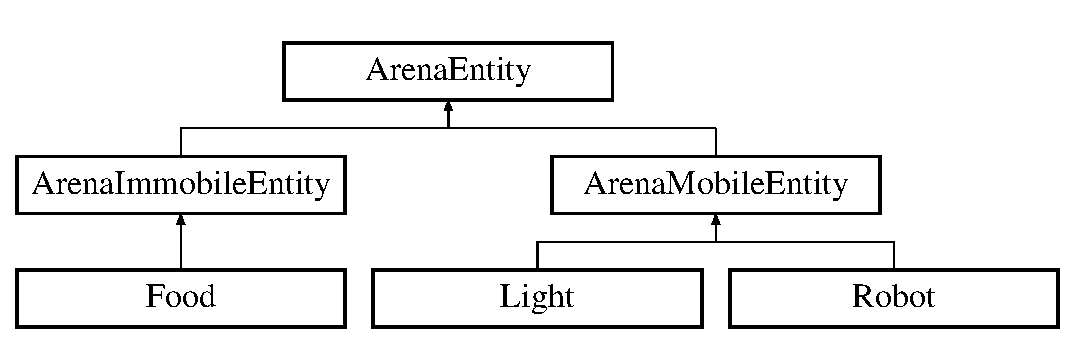
\includegraphics[height=3.000000cm]{class_arena_entity}
\end{center}
\end{figure}
\subsection*{Public Member Functions}
\begin{DoxyCompactItemize}
\item 
\mbox{\Hypertarget{class_arena_entity_a96df749814e89344a6149e4da89b4e44}\label{class_arena_entity_a96df749814e89344a6149e4da89b4e44}} 
\mbox{\hyperlink{class_arena_entity_a96df749814e89344a6149e4da89b4e44}{Arena\+Entity}} ()
\begin{DoxyCompactList}\small\item\em \mbox{\hyperlink{class_arena_entity}{Arena\+Entity}} constructor initialized with default values from \mbox{\hyperlink{params_8h}{params.\+h}}. \end{DoxyCompactList}\item 
\mbox{\Hypertarget{class_arena_entity_aa7af53e5d8830d144ccf2ad07d9140da}\label{class_arena_entity_aa7af53e5d8830d144ccf2ad07d9140da}} 
virtual \mbox{\hyperlink{class_arena_entity_aa7af53e5d8830d144ccf2ad07d9140da}{$\sim$\+Arena\+Entity}} ()=default
\begin{DoxyCompactList}\small\item\em Default destructor -- as defined by compiler. \end{DoxyCompactList}\item 
virtual void \mbox{\hyperlink{class_arena_entity_a203613c40a5cecf47606b2a59adcc3bd}{Timestep\+Update}} (\mbox{\hyperlink{common_8h_a2e3484535ee610c8e19e9859563abe48}{\+\_\+\+\_\+unused}} unsigned int dt)
\begin{DoxyCompactList}\small\item\em Perform whatever updates needed for a particular entity after 1 timestep (updating position, changing color, etc.). \end{DoxyCompactList}\item 
\mbox{\Hypertarget{class_arena_entity_abaebe6c02659e22c08579d49829c5676}\label{class_arena_entity_abaebe6c02659e22c08579d49829c5676}} 
virtual void \mbox{\hyperlink{class_arena_entity_abaebe6c02659e22c08579d49829c5676}{Reset}} ()
\begin{DoxyCompactList}\small\item\em Reset entity to a newly constructed state. \end{DoxyCompactList}\item 
virtual std\+::string \mbox{\hyperlink{class_arena_entity_ad43152003033cf01ad86eeff1990b69a}{get\+\_\+name}} () const =0
\begin{DoxyCompactList}\small\item\em Get the name of the entity for visualization and for debugging. \end{DoxyCompactList}\item 
\mbox{\Hypertarget{class_arena_entity_ab2542a4ed254128e4140333ce5e0b473}\label{class_arena_entity_ab2542a4ed254128e4140333ce5e0b473}} 
virtual void {\bfseries Handle\+Collision} (\mbox{\hyperlink{common_8h_a2e3484535ee610c8e19e9859563abe48}{\+\_\+\+\_\+unused}} Entity\+Type object\+\_\+type, \mbox{\hyperlink{common_8h_a2e3484535ee610c8e19e9859563abe48}{\+\_\+\+\_\+unused}} \mbox{\hyperlink{class_arena_entity}{Arena\+Entity}} $\ast$object=N\+U\+LL)
\item 
\mbox{\Hypertarget{class_arena_entity_a9a0efa995da3ed55e92f54357fd2bdae}\label{class_arena_entity_a9a0efa995da3ed55e92f54357fd2bdae}} 
const \mbox{\hyperlink{struct_pose}{Pose}} \& {\bfseries get\+\_\+pose} () const
\item 
\mbox{\Hypertarget{class_arena_entity_a6eb76e5f1b5949314c12cc512d6930ae}\label{class_arena_entity_a6eb76e5f1b5949314c12cc512d6930ae}} 
void {\bfseries set\+\_\+pose} (const \mbox{\hyperlink{struct_pose}{Pose}} \&pose)
\item 
\mbox{\Hypertarget{class_arena_entity_a3136704edf07c24639319abf5c28dac0}\label{class_arena_entity_a3136704edf07c24639319abf5c28dac0}} 
void \mbox{\hyperlink{class_arena_entity_a3136704edf07c24639319abf5c28dac0}{set\+\_\+position}} (const double inx, const double iny)
\begin{DoxyCompactList}\small\item\em Setter method for position within entity pose variable. \end{DoxyCompactList}\item 
\mbox{\Hypertarget{class_arena_entity_ac1cc3c6997bc7a9573128fc5ded9eb72}\label{class_arena_entity_ac1cc3c6997bc7a9573128fc5ded9eb72}} 
void \mbox{\hyperlink{class_arena_entity_ac1cc3c6997bc7a9573128fc5ded9eb72}{set\+\_\+heading}} (const double t)
\begin{DoxyCompactList}\small\item\em Setter method for heading within entity pose variable. \end{DoxyCompactList}\item 
void \mbox{\hyperlink{class_arena_entity_a4c4bd7f5ffb778979303c33cb3bc9986}{Relative\+Change\+Heading}} (const double delta)
\begin{DoxyCompactList}\small\item\em Setter for heading within pose, but change is relative to current value. \end{DoxyCompactList}\item 
\mbox{\Hypertarget{class_arena_entity_a5790a5d45229aa76223a8183ac916323}\label{class_arena_entity_a5790a5d45229aa76223a8183ac916323}} 
const \mbox{\hyperlink{struct_rgb_color}{Rgb\+Color}} \& {\bfseries get\+\_\+color} () const
\item 
\mbox{\Hypertarget{class_arena_entity_a1ac33beda7462ac5c7f4f71a70d3fb10}\label{class_arena_entity_a1ac33beda7462ac5c7f4f71a70d3fb10}} 
void {\bfseries set\+\_\+color} (const \mbox{\hyperlink{struct_rgb_color}{Rgb\+Color}} \&color)
\item 
\mbox{\Hypertarget{class_arena_entity_a42d86d2d952b7f2a861d8a6cb46e661e}\label{class_arena_entity_a42d86d2d952b7f2a861d8a6cb46e661e}} 
double {\bfseries get\+\_\+radius} () const
\item 
\mbox{\Hypertarget{class_arena_entity_a2b0c2512fe53d143442da5e357f71505}\label{class_arena_entity_a2b0c2512fe53d143442da5e357f71505}} 
void {\bfseries set\+\_\+radius} (double radius)
\item 
\mbox{\Hypertarget{class_arena_entity_a19e75df5ce971f48e9a522a343a39fb3}\label{class_arena_entity_a19e75df5ce971f48e9a522a343a39fb3}} 
Entity\+Type {\bfseries get\+\_\+type} () const
\item 
\mbox{\Hypertarget{class_arena_entity_aa65c584906d4c22f61488fab98c3392c}\label{class_arena_entity_aa65c584906d4c22f61488fab98c3392c}} 
void {\bfseries set\+\_\+type} (Entity\+Type et)
\item 
\mbox{\Hypertarget{class_arena_entity_ae50750dfde8118c27835ea8e9db8b7ef}\label{class_arena_entity_ae50750dfde8118c27835ea8e9db8b7ef}} 
int {\bfseries get\+\_\+id} () const
\item 
\mbox{\Hypertarget{class_arena_entity_a67f4c0467d32eec76ee6ed033ff9ed2f}\label{class_arena_entity_a67f4c0467d32eec76ee6ed033ff9ed2f}} 
void {\bfseries set\+\_\+id} (int id)
\item 
\mbox{\Hypertarget{class_arena_entity_a9cfea21220c07502abd084afde49ae65}\label{class_arena_entity_a9cfea21220c07502abd084afde49ae65}} 
bool \mbox{\hyperlink{class_arena_entity_a9cfea21220c07502abd084afde49ae65}{is\+\_\+mobile}} (void)
\begin{DoxyCompactList}\small\item\em Getter method for determining if entity can move or not. \end{DoxyCompactList}\item 
\mbox{\Hypertarget{class_arena_entity_adb5d3089fec5c28cc989e5834fcdaf6c}\label{class_arena_entity_adb5d3089fec5c28cc989e5834fcdaf6c}} 
void \mbox{\hyperlink{class_arena_entity_adb5d3089fec5c28cc989e5834fcdaf6c}{set\+\_\+mobility}} (bool value)
\begin{DoxyCompactList}\small\item\em Setter method for indicating if entity can move or not. \end{DoxyCompactList}\end{DoxyCompactItemize}


\subsection{Detailed Description}
A food class from which all \mbox{\hyperlink{class_arena}{Arena}} entities inherit. 

All entities know how to\+:


\begin{DoxyEnumerate}
\item Update themselves at each timestep (i.\+e. in accordance with current velocity and position).
\item Reset themselves to a newly constructed state. So that the user can click the reset button to restart the game. Alternatively, the game will be reset if the robot has won/lost.
\end{DoxyEnumerate}

Please note that here use the upper-\/left coordinate, which means that the origin point (0.\+0,0.\+0) is at the upper left.

All arena entities are circular. 

\subsection{Member Function Documentation}
\mbox{\Hypertarget{class_arena_entity_ad43152003033cf01ad86eeff1990b69a}\label{class_arena_entity_ad43152003033cf01ad86eeff1990b69a}} 
\index{Arena\+Entity@{Arena\+Entity}!get\+\_\+name@{get\+\_\+name}}
\index{get\+\_\+name@{get\+\_\+name}!Arena\+Entity@{Arena\+Entity}}
\subsubsection{\texorpdfstring{get\+\_\+name()}{get\_name()}}
{\footnotesize\ttfamily virtual std\+::string Arena\+Entity\+::get\+\_\+name (\begin{DoxyParamCaption}{ }\end{DoxyParamCaption}) const\hspace{0.3cm}{\ttfamily [pure virtual]}}



Get the name of the entity for visualization and for debugging. 

\begin{DoxyReturn}{Returns}
Name of the entity. Each entity type hard codes its name (e.\+g. \char`\"{}\+Robot\char`\"{}). 
\end{DoxyReturn}


Implemented in \mbox{\hyperlink{class_robot_a3f77c13705b8f60480d21d8d936dc39e}{Robot}}, \mbox{\hyperlink{class_food_a5c3bcd5109750a15ebb24b8a2a3cdd07}{Food}}, and \mbox{\hyperlink{class_light_a49b2e32cf8173353ac4689fdadbb95d5}{Light}}.

\mbox{\Hypertarget{class_arena_entity_a4c4bd7f5ffb778979303c33cb3bc9986}\label{class_arena_entity_a4c4bd7f5ffb778979303c33cb3bc9986}} 
\index{Arena\+Entity@{Arena\+Entity}!Relative\+Change\+Heading@{Relative\+Change\+Heading}}
\index{Relative\+Change\+Heading@{Relative\+Change\+Heading}!Arena\+Entity@{Arena\+Entity}}
\subsubsection{\texorpdfstring{Relative\+Change\+Heading()}{RelativeChangeHeading()}}
{\footnotesize\ttfamily void Arena\+Entity\+::\+Relative\+Change\+Heading (\begin{DoxyParamCaption}\item[{const double}]{delta }\end{DoxyParamCaption})\hspace{0.3cm}{\ttfamily [inline]}}



Setter for heading within pose, but change is relative to current value. 


\begin{DoxyParams}[1]{Parameters}
\mbox{\tt in}  & {\em delta} & by which to modify current heading. Can be positive or negative. \\
\hline
\end{DoxyParams}
\mbox{\Hypertarget{class_arena_entity_a203613c40a5cecf47606b2a59adcc3bd}\label{class_arena_entity_a203613c40a5cecf47606b2a59adcc3bd}} 
\index{Arena\+Entity@{Arena\+Entity}!Timestep\+Update@{Timestep\+Update}}
\index{Timestep\+Update@{Timestep\+Update}!Arena\+Entity@{Arena\+Entity}}
\subsubsection{\texorpdfstring{Timestep\+Update()}{TimestepUpdate()}}
{\footnotesize\ttfamily virtual void Arena\+Entity\+::\+Timestep\+Update (\begin{DoxyParamCaption}\item[{\mbox{\hyperlink{common_8h_a2e3484535ee610c8e19e9859563abe48}{\+\_\+\+\_\+unused}} unsigned int}]{dt }\end{DoxyParamCaption})\hspace{0.3cm}{\ttfamily [inline]}, {\ttfamily [virtual]}}



Perform whatever updates needed for a particular entity after 1 timestep (updating position, changing color, etc.). 


\begin{DoxyParams}[1]{Parameters}
\mbox{\tt in}  & {\em dt} & is time elapsed since the last update. Unused. \\
\hline
\end{DoxyParams}


The documentation for this class was generated from the following file\+:\begin{DoxyCompactItemize}
\item 
src/\mbox{\hyperlink{arena__entity_8h}{arena\+\_\+entity.\+h}}\end{DoxyCompactItemize}

\hypertarget{class_arena_immobile_entity}{}\section{Arena\+Immobile\+Entity Class Reference}
\label{class_arena_immobile_entity}\index{Arena\+Immobile\+Entity@{Arena\+Immobile\+Entity}}


An immobile entity in the \mbox{\hyperlink{class_arena}{Arena}}.  




{\ttfamily \#include $<$arena\+\_\+immobile\+\_\+entity.\+h$>$}

Inheritance diagram for Arena\+Immobile\+Entity\+:\begin{figure}[H]
\begin{center}
\leavevmode
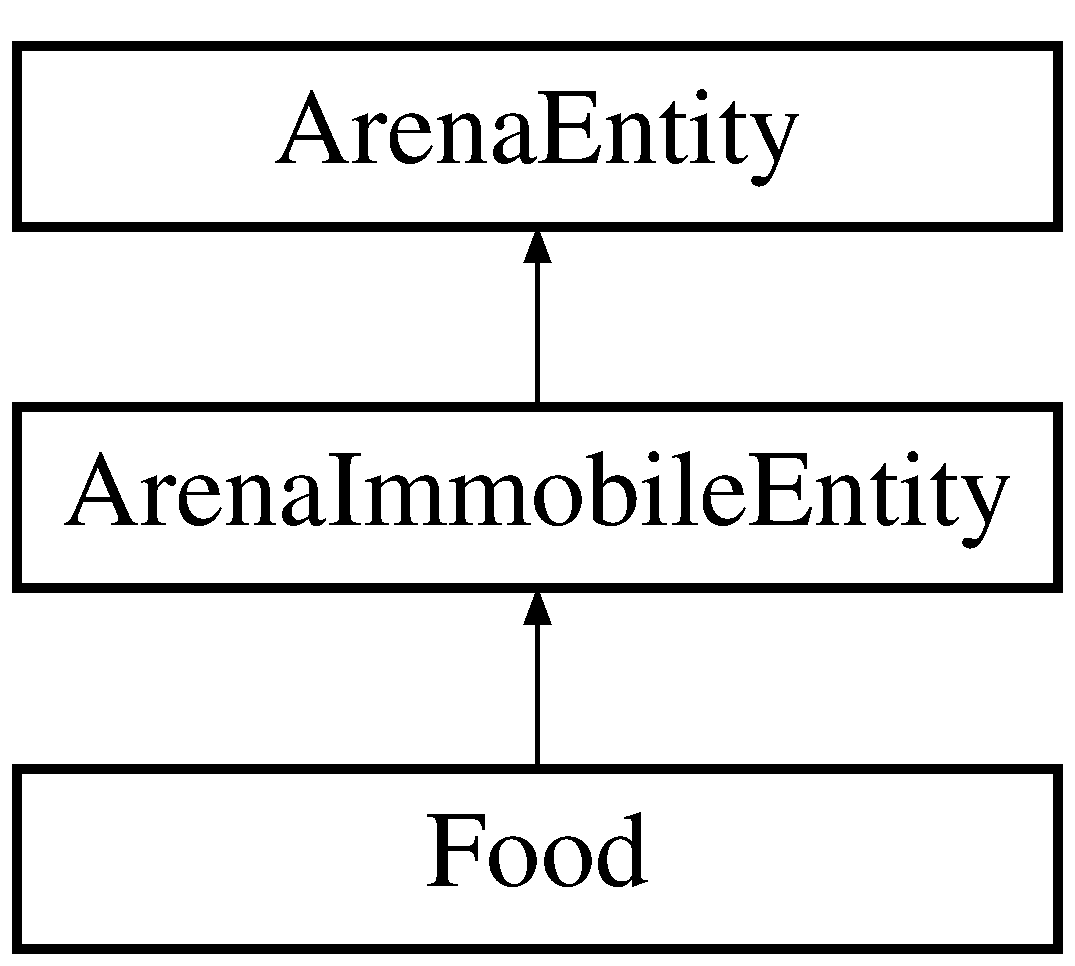
\includegraphics[height=3.000000cm]{class_arena_immobile_entity}
\end{center}
\end{figure}
\subsection*{Public Member Functions}
\begin{DoxyCompactItemize}
\item 
\mbox{\hyperlink{class_arena_immobile_entity_ac24bb0af97a140d62dd52124489032fd}{Arena\+Immobile\+Entity}} ()
\begin{DoxyCompactList}\small\item\em \mbox{\hyperlink{class_arena_immobile_entity}{Arena\+Immobile\+Entity}}\textquotesingle{}s constructor. \end{DoxyCompactList}\end{DoxyCompactItemize}


\subsection{Detailed Description}
An immobile entity in the \mbox{\hyperlink{class_arena}{Arena}}. 

Immobile entities cannot move, and therefore do not need to override the \mbox{\hyperlink{class_arena_entity_a203613c40a5cecf47606b2a59adcc3bd}{Timestep\+Update()}} function. 

\subsection{Constructor \& Destructor Documentation}
\mbox{\Hypertarget{class_arena_immobile_entity_ac24bb0af97a140d62dd52124489032fd}\label{class_arena_immobile_entity_ac24bb0af97a140d62dd52124489032fd}} 
\index{Arena\+Immobile\+Entity@{Arena\+Immobile\+Entity}!Arena\+Immobile\+Entity@{Arena\+Immobile\+Entity}}
\index{Arena\+Immobile\+Entity@{Arena\+Immobile\+Entity}!Arena\+Immobile\+Entity@{Arena\+Immobile\+Entity}}
\subsubsection{\texorpdfstring{Arena\+Immobile\+Entity()}{ArenaImmobileEntity()}}
{\footnotesize\ttfamily Arena\+Immobile\+Entity\+::\+Arena\+Immobile\+Entity (\begin{DoxyParamCaption}{ }\end{DoxyParamCaption})\hspace{0.3cm}{\ttfamily [inline]}}



\mbox{\hyperlink{class_arena_immobile_entity}{Arena\+Immobile\+Entity}}\textquotesingle{}s constructor. 


\begin{DoxyParams}{Parameters}
{\em radius} & The radius of the entity (as it is circular). \\
\hline
{\em pos} & The initial position of the entity. \\
\hline
{\em color} & The color of the entity as shown on the screen. \\
\hline
\end{DoxyParams}


The documentation for this class was generated from the following file\+:\begin{DoxyCompactItemize}
\item 
src/\mbox{\hyperlink{arena__immobile__entity_8h}{arena\+\_\+immobile\+\_\+entity.\+h}}\end{DoxyCompactItemize}

\hypertarget{class_arena_mobile_entity}{}\section{Arena\+Mobile\+Entity Class Reference}
\label{class_arena_mobile_entity}\index{Arena\+Mobile\+Entity@{Arena\+Mobile\+Entity}}


A mobile entity in the \mbox{\hyperlink{class_arena}{Arena}}, capable of updating its own position and/or velocity when asked by the simulation.  




{\ttfamily \#include $<$arena\+\_\+mobile\+\_\+entity.\+h$>$}

Inheritance diagram for Arena\+Mobile\+Entity\+:\begin{figure}[H]
\begin{center}
\leavevmode
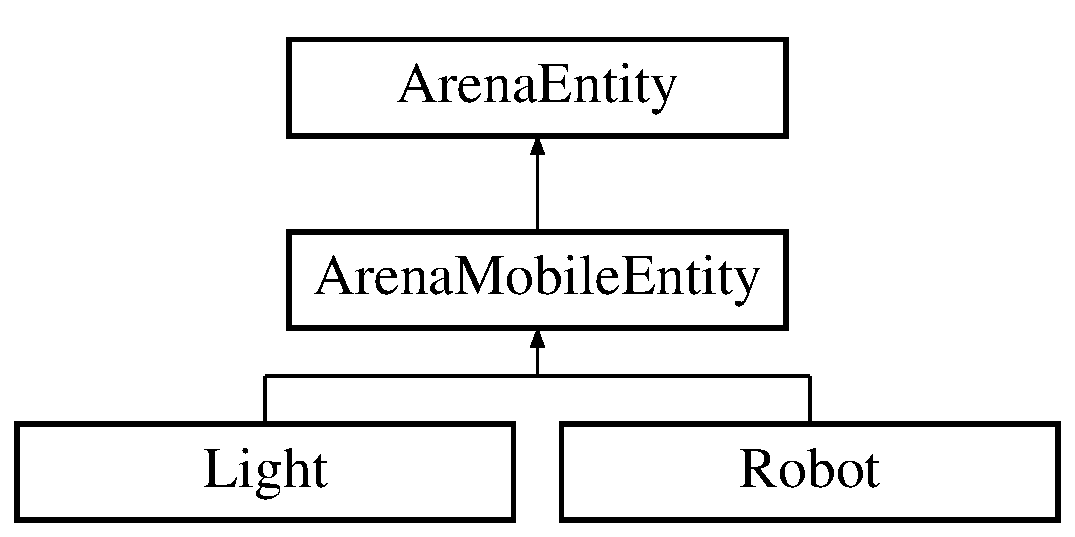
\includegraphics[height=3.000000cm]{class_arena_mobile_entity}
\end{center}
\end{figure}
\subsection*{Public Member Functions}
\begin{DoxyCompactItemize}
\item 
\mbox{\Hypertarget{class_arena_mobile_entity_a6d038ac71d9b149052fc5a0fec4907f9}\label{class_arena_mobile_entity_a6d038ac71d9b149052fc5a0fec4907f9}} 
\mbox{\hyperlink{class_arena_mobile_entity_a6d038ac71d9b149052fc5a0fec4907f9}{Arena\+Mobile\+Entity}} ()
\begin{DoxyCompactList}\small\item\em \mbox{\hyperlink{class_arena_mobile_entity}{Arena\+Mobile\+Entity}}\textquotesingle{}s constructor. \end{DoxyCompactList}\item 
\mbox{\Hypertarget{class_arena_mobile_entity_ad662f3efc1a56b64ecaf5633e7ff2139}\label{class_arena_mobile_entity_ad662f3efc1a56b64ecaf5633e7ff2139}} 
{\bfseries Arena\+Mobile\+Entity} (const \mbox{\hyperlink{class_arena_mobile_entity}{Arena\+Mobile\+Entity}} \&other)=delete
\item 
\mbox{\Hypertarget{class_arena_mobile_entity_a34a7f0d094515cafff7611a0f6cf4eee}\label{class_arena_mobile_entity_a34a7f0d094515cafff7611a0f6cf4eee}} 
\mbox{\hyperlink{class_arena_mobile_entity}{Arena\+Mobile\+Entity}} \& {\bfseries operator=} (const \mbox{\hyperlink{class_arena_mobile_entity}{Arena\+Mobile\+Entity}} \&other)=delete
\item 
\mbox{\Hypertarget{class_arena_mobile_entity_a2116341414a3ad0449dc03efa6ea500b}\label{class_arena_mobile_entity_a2116341414a3ad0449dc03efa6ea500b}} 
virtual double {\bfseries get\+\_\+speed} ()
\item 
\mbox{\Hypertarget{class_arena_mobile_entity_a1a047f4377a9557516a2e1d6d73db849}\label{class_arena_mobile_entity_a1a047f4377a9557516a2e1d6d73db849}} 
virtual void {\bfseries set\+\_\+speed} (double sp)
\item 
\mbox{\Hypertarget{class_arena_mobile_entity_ae9507f1b0c6bfdfd62afbab8a9a150f7}\label{class_arena_mobile_entity_ae9507f1b0c6bfdfd62afbab8a9a150f7}} 
\mbox{\hyperlink{class_sensor_touch}{Sensor\+Touch}} $\ast$ \mbox{\hyperlink{class_arena_mobile_entity_ae9507f1b0c6bfdfd62afbab8a9a150f7}{get\+\_\+touch\+\_\+sensor}} ()
\begin{DoxyCompactList}\small\item\em Get a pointer to the \mbox{\hyperlink{class_arena_mobile_entity}{Arena\+Mobile\+Entity}}\textquotesingle{}s touch sensor. \end{DoxyCompactList}\end{DoxyCompactItemize}
\subsection*{Protected Attributes}
\begin{DoxyCompactItemize}
\item 
\mbox{\Hypertarget{class_arena_mobile_entity_a260fd3fba196ee9ab56f9f2ce6ab4a21}\label{class_arena_mobile_entity_a260fd3fba196ee9ab56f9f2ce6ab4a21}} 
\mbox{\hyperlink{class_sensor_touch}{Sensor\+Touch}} $\ast$ {\bfseries sensor\+\_\+touch\+\_\+}
\end{DoxyCompactItemize}


\subsection{Detailed Description}
A mobile entity in the \mbox{\hyperlink{class_arena}{Arena}}, capable of updating its own position and/or velocity when asked by the simulation. 

All mobile entities must have a heading angle so that their orientation can be properly drawn by the \mbox{\hyperlink{class_graphics_arena_viewer}{Graphics\+Arena\+Viewer}}.

Since this is also a food class, many of its methods are intuitively {\ttfamily virtual}. 

The documentation for this class was generated from the following file\+:\begin{DoxyCompactItemize}
\item 
src/\mbox{\hyperlink{arena__mobile__entity_8h}{arena\+\_\+mobile\+\_\+entity.\+h}}\end{DoxyCompactItemize}

\hypertarget{class_controller}{}\section{Controller Class Reference}
\label{class_controller}\index{Controller@{Controller}}


\mbox{\hyperlink{class_controller}{Controller}} that mediates \mbox{\hyperlink{class_arena}{Arena}} and \mbox{\hyperlink{class_graphics_arena_viewer}{Graphics\+Arena\+Viewer}} communication.  




{\ttfamily \#include $<$controller.\+h$>$}

\subsection*{Public Member Functions}
\begin{DoxyCompactItemize}
\item 
\mbox{\Hypertarget{class_controller_a95c56822d667e94b031451729ce069a9}\label{class_controller_a95c56822d667e94b031451729ce069a9}} 
\mbox{\hyperlink{class_controller_a95c56822d667e94b031451729ce069a9}{Controller}} ()
\begin{DoxyCompactList}\small\item\em \mbox{\hyperlink{class_controller}{Controller}}\textquotesingle{}s constructor that will create \mbox{\hyperlink{class_arena}{Arena}} and Viewer. \end{DoxyCompactList}\item 
\mbox{\Hypertarget{class_controller_a17abb2cec6c0109e9b2df3cdc082eaad}\label{class_controller_a17abb2cec6c0109e9b2df3cdc082eaad}} 
void \mbox{\hyperlink{class_controller_a17abb2cec6c0109e9b2df3cdc082eaad}{Run}} ()
\begin{DoxyCompactList}\small\item\em Run launches the graphics and starts the game. \end{DoxyCompactList}\item 
\mbox{\Hypertarget{class_controller_a6a4a3eaee03f6c4718da3f8293d7e053}\label{class_controller_a6a4a3eaee03f6c4718da3f8293d7e053}} 
void \mbox{\hyperlink{class_controller_a6a4a3eaee03f6c4718da3f8293d7e053}{Advance\+Time}} (double dt)
\begin{DoxyCompactList}\small\item\em Advance\+Time is communication from the Viewer to advance the simulation. \end{DoxyCompactList}\item 
\mbox{\Hypertarget{class_controller_a55b8d46984535adb91f40309914e8852}\label{class_controller_a55b8d46984535adb91f40309914e8852}} 
void \mbox{\hyperlink{class_controller_a55b8d46984535adb91f40309914e8852}{Accept\+Communication}} (Communication com)
\begin{DoxyCompactList}\small\item\em Accept\+Communication from either the viewer or the \mbox{\hyperlink{class_arena}{Arena}}. \end{DoxyCompactList}\item 
\mbox{\Hypertarget{class_controller_a9cd0e53064f5cae41d8cf2aaeee81055}\label{class_controller_a9cd0e53064f5cae41d8cf2aaeee81055}} 
void {\bfseries Accept\+Communication\+Up} (Communication com)
\item 
Communication \mbox{\hyperlink{class_controller_ae9b0504ab74cdacc654528b609074adc}{Convert\+Comm}} (Communication com)
\begin{DoxyCompactList}\small\item\em Converts the communication from one to send to the other. \end{DoxyCompactList}\end{DoxyCompactItemize}


\subsection{Detailed Description}
\mbox{\hyperlink{class_controller}{Controller}} that mediates \mbox{\hyperlink{class_arena}{Arena}} and \mbox{\hyperlink{class_graphics_arena_viewer}{Graphics\+Arena\+Viewer}} communication. 

The \mbox{\hyperlink{class_controller}{Controller}} instantiates the \mbox{\hyperlink{class_arena}{Arena}} and the \mbox{\hyperlink{class_graphics_arena_viewer}{Graphics\+Arena\+Viewer}}. The viewer contains the main loop that keeps it live, but at each update, the viewer sends a message to the controller to update its time.

Other types of communication between \mbox{\hyperlink{class_arena}{Arena}} and Viewer include\+:
\begin{DoxyItemize}
\item keypresses intercepted by the Viewer.
\item Play/\+Pause/\+New Game user input via the Viewer.
\item Game status from arena to the viewer. 
\end{DoxyItemize}

\subsection{Member Function Documentation}
\mbox{\Hypertarget{class_controller_ae9b0504ab74cdacc654528b609074adc}\label{class_controller_ae9b0504ab74cdacc654528b609074adc}} 
\index{Controller@{Controller}!Convert\+Comm@{Convert\+Comm}}
\index{Convert\+Comm@{Convert\+Comm}!Controller@{Controller}}
\subsubsection{\texorpdfstring{Convert\+Comm()}{ConvertComm()}}
{\footnotesize\ttfamily Communication Controller\+::\+Convert\+Comm (\begin{DoxyParamCaption}\item[{Communication}]{com }\end{DoxyParamCaption})}



Converts the communication from one to send to the other. 

Used primarily for testing purposes to insure communication is being correctly received, interpreted, and relayed.

Converts communication from one source to appropriate communication to the other source. For example, the viewer sends a k\+Key\+Up communication, and this translate to a k\+Increase\+Speed communication to \mbox{\hyperlink{class_arena}{Arena}}.\+: Complete the conversion code for all key presses. 

The documentation for this class was generated from the following files\+:\begin{DoxyCompactItemize}
\item 
src/\mbox{\hyperlink{controller_8h}{controller.\+h}}\item 
src/\mbox{\hyperlink{controller_8cc}{controller.\+cc}}\end{DoxyCompactItemize}

\hypertarget{class_entity_factory}{}\section{Entity\+Factory Class Reference}
\label{class_entity_factory}\index{Entity\+Factory@{Entity\+Factory}}


A factory for the instantiation of all types of arena entities.  




{\ttfamily \#include $<$entity\+\_\+factory.\+h$>$}

\subsection*{Public Member Functions}
\begin{DoxyCompactItemize}
\item 
\mbox{\hyperlink{class_entity_factory_abaf0c4ceaa682e55f69b0ceae230008a}{Entity\+Factory}} ()
\begin{DoxyCompactList}\small\item\em \mbox{\hyperlink{class_entity_factory}{Entity\+Factory}} constructor. \end{DoxyCompactList}\item 
\mbox{\Hypertarget{class_entity_factory_ae3246f06fa101178803f76582323d4ad}\label{class_entity_factory_ae3246f06fa101178803f76582323d4ad}} 
virtual \mbox{\hyperlink{class_entity_factory_ae3246f06fa101178803f76582323d4ad}{$\sim$\+Entity\+Factory}} ()=default
\begin{DoxyCompactList}\small\item\em Default destructor. \end{DoxyCompactList}\item 
\mbox{\hyperlink{class_arena_entity}{Arena\+Entity}} $\ast$ \mbox{\hyperlink{class_entity_factory_abf7b1ac4ec275728b47c37fcd85f81e8}{Create\+Entity}} (Entity\+Type etype)
\begin{DoxyCompactList}\small\item\em Create\+Entity is primary purpose of this class. \end{DoxyCompactList}\end{DoxyCompactItemize}
\subsection*{Public Attributes}
\begin{DoxyCompactItemize}
\item 
\mbox{\Hypertarget{class_entity_factory_aa53d4bb51d0cd74024080b87e42577f9}\label{class_entity_factory_aa53d4bb51d0cd74024080b87e42577f9}} 
int {\bfseries entity\+\_\+count\+\_\+} \{0\}
\item 
\mbox{\Hypertarget{class_entity_factory_a4142b8531802417f4dda36c297c5c05e}\label{class_entity_factory_a4142b8531802417f4dda36c297c5c05e}} 
int {\bfseries robot\+\_\+count\+\_\+} \{0\}
\item 
\mbox{\Hypertarget{class_entity_factory_aefd32f0dd502d7eedaefe8a0f245992f}\label{class_entity_factory_aefd32f0dd502d7eedaefe8a0f245992f}} 
int {\bfseries light\+\_\+count\+\_\+} \{0\}
\item 
\mbox{\Hypertarget{class_entity_factory_a932b4b34f1b5d592488520c9ce004810}\label{class_entity_factory_a932b4b34f1b5d592488520c9ce004810}} 
int {\bfseries food\+\_\+count\+\_\+} \{0\}
\item 
\mbox{\Hypertarget{class_entity_factory_af7ae85b5eebd8c9d1b6015cd89936e65}\label{class_entity_factory_af7ae85b5eebd8c9d1b6015cd89936e65}} 
int {\bfseries fear\+\_\+count\+\_\+} \{5\}
\item 
\mbox{\Hypertarget{class_entity_factory_a117adf5c2d5033c26294c5e0db3c0eda}\label{class_entity_factory_a117adf5c2d5033c26294c5e0db3c0eda}} 
int {\bfseries sense} \{1\}
\end{DoxyCompactItemize}


\subsection{Detailed Description}
A factory for the instantiation of all types of arena entities. 

The factory keeps track of the number of entities of each type and overall. It assigns ID\textquotesingle{}s to the entity when it creates it. The factory randomly places entities, and in doing so, attempts to not have them overlap. 

\subsection{Constructor \& Destructor Documentation}
\mbox{\Hypertarget{class_entity_factory_abaf0c4ceaa682e55f69b0ceae230008a}\label{class_entity_factory_abaf0c4ceaa682e55f69b0ceae230008a}} 
\index{Entity\+Factory@{Entity\+Factory}!Entity\+Factory@{Entity\+Factory}}
\index{Entity\+Factory@{Entity\+Factory}!Entity\+Factory@{Entity\+Factory}}
\subsubsection{\texorpdfstring{Entity\+Factory()}{EntityFactory()}}
{\footnotesize\ttfamily Entity\+Factory\+::\+Entity\+Factory (\begin{DoxyParamCaption}{ }\end{DoxyParamCaption})}



\mbox{\hyperlink{class_entity_factory}{Entity\+Factory}} constructor. 



\subsection{Member Function Documentation}
\mbox{\Hypertarget{class_entity_factory_abf7b1ac4ec275728b47c37fcd85f81e8}\label{class_entity_factory_abf7b1ac4ec275728b47c37fcd85f81e8}} 
\index{Entity\+Factory@{Entity\+Factory}!Create\+Entity@{Create\+Entity}}
\index{Create\+Entity@{Create\+Entity}!Entity\+Factory@{Entity\+Factory}}
\subsubsection{\texorpdfstring{Create\+Entity()}{CreateEntity()}}
{\footnotesize\ttfamily \mbox{\hyperlink{class_arena_entity}{Arena\+Entity}} $\ast$ Entity\+Factory\+::\+Create\+Entity (\begin{DoxyParamCaption}\item[{Entity\+Type}]{etype }\end{DoxyParamCaption})}



Create\+Entity is primary purpose of this class. 


\begin{DoxyParams}[1]{Parameters}
\mbox{\tt in}  & {\em etype} & The type to make. \\
\hline
\mbox{\tt out}  & {\em new} & dynamically created entity.\\
\hline
\end{DoxyParams}
Currently, the \mbox{\hyperlink{class_arena}{Arena}} gets the entity and places it in the appropriate data structure. It might be useful to instead have the factory place on the appropriate data structure so that the call to \mbox{\hyperlink{class_arena}{Arena}} is the same regardless of the entity type. 

The documentation for this class was generated from the following files\+:\begin{DoxyCompactItemize}
\item 
src/\mbox{\hyperlink{entity__factory_8h}{entity\+\_\+factory.\+h}}\item 
src/\mbox{\hyperlink{entity__factory_8cc}{entity\+\_\+factory.\+cc}}\end{DoxyCompactItemize}

\hypertarget{class_food}{}\section{Food Class Reference}
\label{class_food}\index{Food@{Food}}


Class representing a immobile food within the \mbox{\hyperlink{class_arena}{Arena}}.  




{\ttfamily \#include $<$food.\+h$>$}

Inheritance diagram for Food\+:\begin{figure}[H]
\begin{center}
\leavevmode
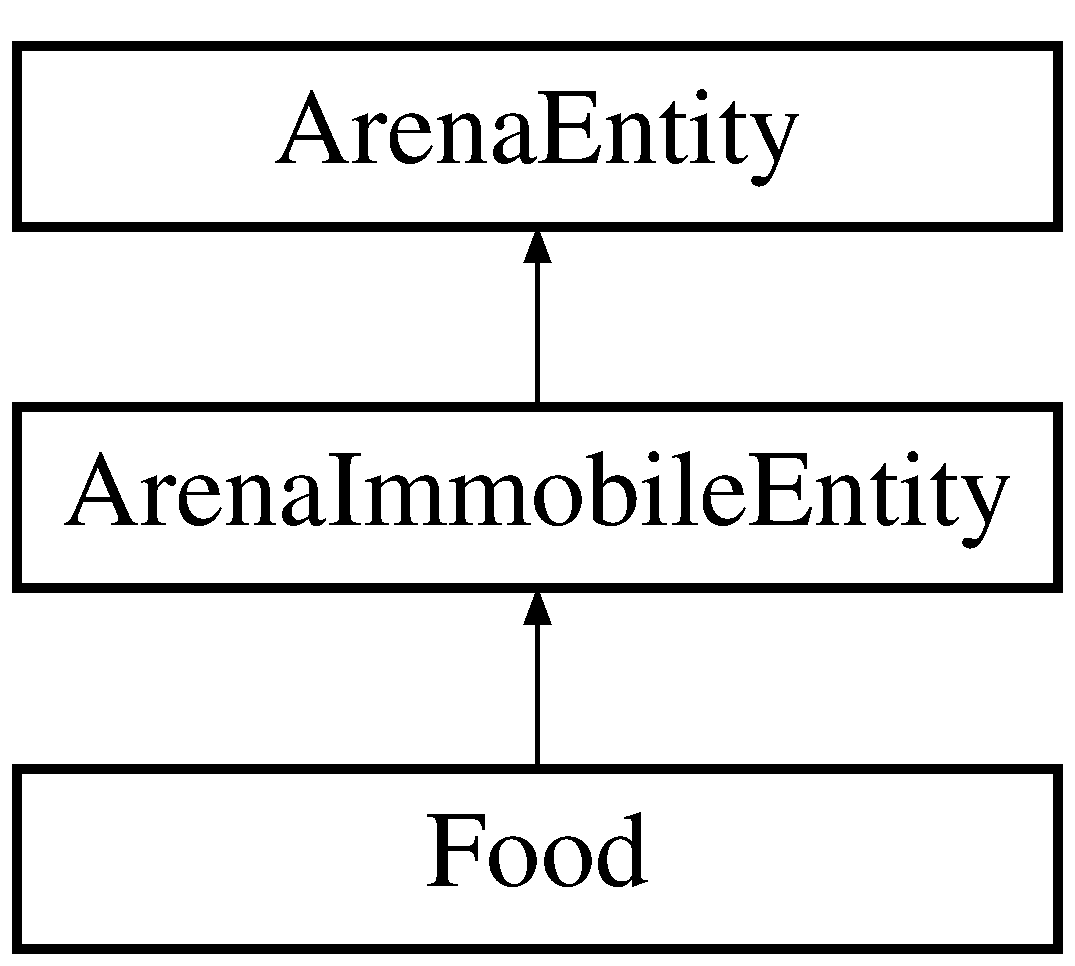
\includegraphics[height=3.000000cm]{class_food}
\end{center}
\end{figure}
\subsection*{Public Member Functions}
\begin{DoxyCompactItemize}
\item 
\mbox{\hyperlink{class_food_a75d4d7f76fd495cc8133302ca9fdc485}{Food}} ()
\begin{DoxyCompactList}\small\item\em Constructor. \end{DoxyCompactList}\item 
\mbox{\Hypertarget{class_food_a1a12bfd50400e04b595c24a512317c1a}\label{class_food_a1a12bfd50400e04b595c24a512317c1a}} 
void \mbox{\hyperlink{class_food_a1a12bfd50400e04b595c24a512317c1a}{Reset}} () override
\begin{DoxyCompactList}\small\item\em Reset the \mbox{\hyperlink{class_food}{Food}} using the initialization parameters received by the constructor. \end{DoxyCompactList}\item 
std\+::string \mbox{\hyperlink{class_food_a5c3bcd5109750a15ebb24b8a2a3cdd07}{get\+\_\+name}} () const override
\begin{DoxyCompactList}\small\item\em Get the name of the \mbox{\hyperlink{class_food}{Food}} for visualization purposes, and to aid in debugging. \end{DoxyCompactList}\item 
bool \mbox{\hyperlink{class_food_a81c160e9e591b4a4eb9662efb7130ee8}{Is\+Captured}} () const
\begin{DoxyCompactList}\small\item\em Getter for captured\+\_\+, which is the state of the food. \end{DoxyCompactList}\item 
\mbox{\Hypertarget{class_food_a1ad8a3c17f9ab764215320ec11c7c40d}\label{class_food_a1ad8a3c17f9ab764215320ec11c7c40d}} 
void \mbox{\hyperlink{class_food_a1ad8a3c17f9ab764215320ec11c7c40d}{set\+\_\+captured}} (bool state)
\begin{DoxyCompactList}\small\item\em Setter for captured\+\_\+, which is the state of the food. \end{DoxyCompactList}\end{DoxyCompactItemize}


\subsection{Detailed Description}
Class representing a immobile food within the \mbox{\hyperlink{class_arena}{Arena}}. 

\mbox{\hyperlink{class_food}{Food}} can enhance a \mbox{\hyperlink{class_robot}{Robot}}. If a \mbox{\hyperlink{class_robot}{Robot}} touches the \mbox{\hyperlink{class_food}{Food}}, it becomes a super robot.

\mbox{\hyperlink{class_food}{Food}} have the capability of updating their own position when asked, and also track their own velocity and heading. They have a touch sensor for responding to collision events which is activated/deactivated on collision events. 

\subsection{Constructor \& Destructor Documentation}
\mbox{\Hypertarget{class_food_a75d4d7f76fd495cc8133302ca9fdc485}\label{class_food_a75d4d7f76fd495cc8133302ca9fdc485}} 
\index{Food@{Food}!Food@{Food}}
\index{Food@{Food}!Food@{Food}}
\subsubsection{\texorpdfstring{Food()}{Food()}}
{\footnotesize\ttfamily Food\+::\+Food (\begin{DoxyParamCaption}{ }\end{DoxyParamCaption})}



Constructor. 


\begin{DoxyParams}{Parameters}
{\em params} & A food\+\_\+params passed down from \mbox{\hyperlink{main_8cc}{main.\+cc}} for the initialization of the \mbox{\hyperlink{class_food}{Food}}. \\
\hline
\end{DoxyParams}


\subsection{Member Function Documentation}
\mbox{\Hypertarget{class_food_a5c3bcd5109750a15ebb24b8a2a3cdd07}\label{class_food_a5c3bcd5109750a15ebb24b8a2a3cdd07}} 
\index{Food@{Food}!get\+\_\+name@{get\+\_\+name}}
\index{get\+\_\+name@{get\+\_\+name}!Food@{Food}}
\subsubsection{\texorpdfstring{get\+\_\+name()}{get\_name()}}
{\footnotesize\ttfamily std\+::string Food\+::get\+\_\+name (\begin{DoxyParamCaption}{ }\end{DoxyParamCaption}) const\hspace{0.3cm}{\ttfamily [inline]}, {\ttfamily [override]}, {\ttfamily [virtual]}}



Get the name of the \mbox{\hyperlink{class_food}{Food}} for visualization purposes, and to aid in debugging. 

\begin{DoxyReturn}{Returns}
Name of the \mbox{\hyperlink{class_food}{Food}}. 
\end{DoxyReturn}


Implements \mbox{\hyperlink{class_arena_entity_ad43152003033cf01ad86eeff1990b69a}{Arena\+Entity}}.

\mbox{\Hypertarget{class_food_a81c160e9e591b4a4eb9662efb7130ee8}\label{class_food_a81c160e9e591b4a4eb9662efb7130ee8}} 
\index{Food@{Food}!Is\+Captured@{Is\+Captured}}
\index{Is\+Captured@{Is\+Captured}!Food@{Food}}
\subsubsection{\texorpdfstring{Is\+Captured()}{IsCaptured()}}
{\footnotesize\ttfamily bool Food\+::\+Is\+Captured (\begin{DoxyParamCaption}{ }\end{DoxyParamCaption}) const\hspace{0.3cm}{\ttfamily [inline]}}



Getter for captured\+\_\+, which is the state of the food. 

\begin{DoxyReturn}{Returns}
true if captured. 
\end{DoxyReturn}


The documentation for this class was generated from the following files\+:\begin{DoxyCompactItemize}
\item 
src/\mbox{\hyperlink{food_8h}{food.\+h}}\item 
src/\mbox{\hyperlink{food_8cc}{food.\+cc}}\end{DoxyCompactItemize}

\hypertarget{class_food_sensor}{}\section{Food\+Sensor Class Reference}
\label{class_food_sensor}\index{Food\+Sensor@{Food\+Sensor}}


Class representing a \mbox{\hyperlink{class_food}{Food}} sensor.  




{\ttfamily \#include $<$food\+\_\+sensor.\+h$>$}

Inheritance diagram for Food\+Sensor\+:\begin{figure}[H]
\begin{center}
\leavevmode
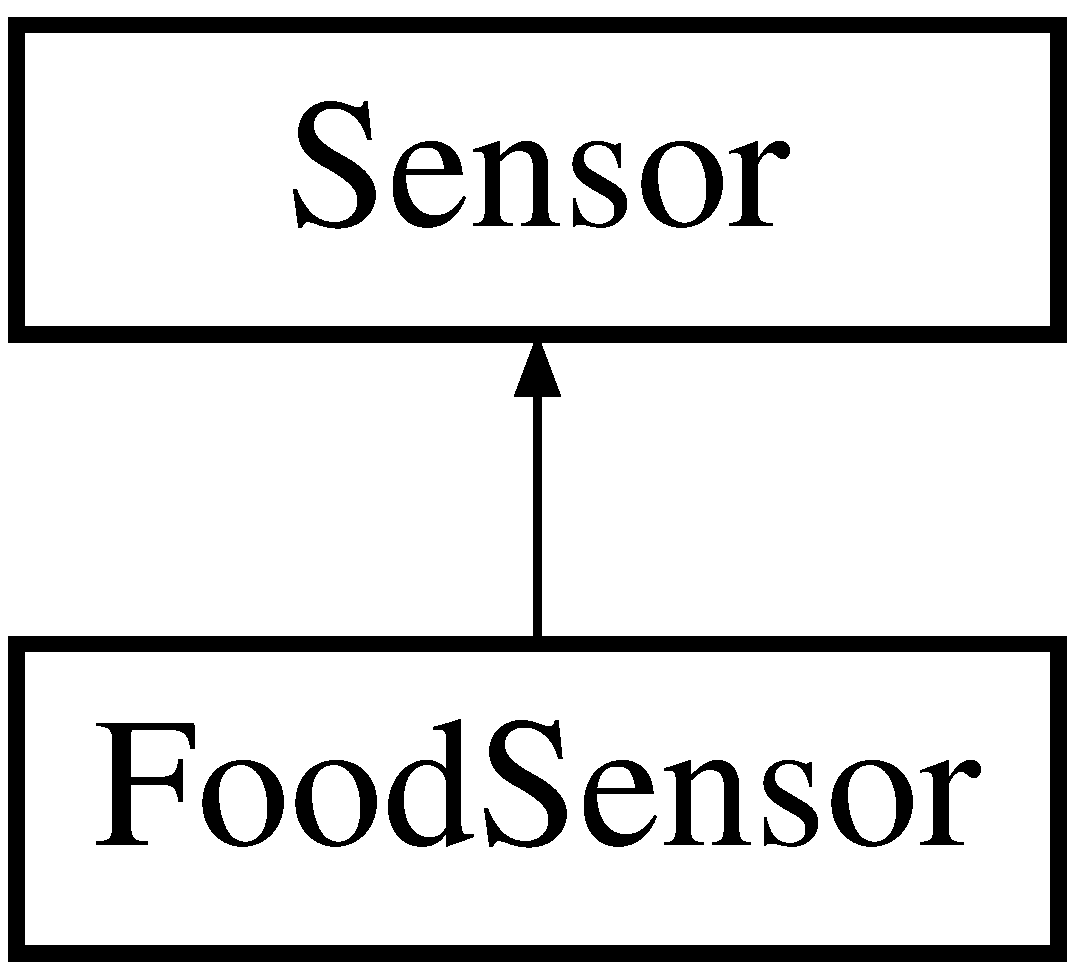
\includegraphics[height=2.000000cm]{class_food_sensor}
\end{center}
\end{figure}
\subsection*{Public Member Functions}
\begin{DoxyCompactItemize}
\item 
\mbox{\Hypertarget{class_food_sensor_a682d81dbb4bef2c726ef7df1b7309508}\label{class_food_sensor_a682d81dbb4bef2c726ef7df1b7309508}} 
{\bfseries Food\+Sensor} (int xpos, int ypos)
\end{DoxyCompactItemize}


\subsection{Detailed Description}
Class representing a \mbox{\hyperlink{class_food}{Food}} sensor. 

This is a \mbox{\hyperlink{class_food}{Food}} sensor class that takes in the the position of the entity being sensed it then calculates the reading based on the position of that entity and its own position which it holds. This class inherits from base sensor and most of the work is done in that class. Sensors are fed readings and return them when prompted. 

The documentation for this class was generated from the following file\+:\begin{DoxyCompactItemize}
\item 
src/food\+\_\+sensor.\+h\end{DoxyCompactItemize}

\hypertarget{class_graphics_arena_viewer}{}\section{Graphics\+Arena\+Viewer Class Reference}
\label{class_graphics_arena_viewer}\index{Graphics\+Arena\+Viewer@{Graphics\+Arena\+Viewer}}


An application that uses the Min\+Gfx library to open up a window that includes a few buttons for controlling the simulation and can be used to draw circles and other computer graphics.  




{\ttfamily \#include $<$graphics\+\_\+arena\+\_\+viewer.\+h$>$}

Inheritance diagram for Graphics\+Arena\+Viewer\+:\begin{figure}[H]
\begin{center}
\leavevmode
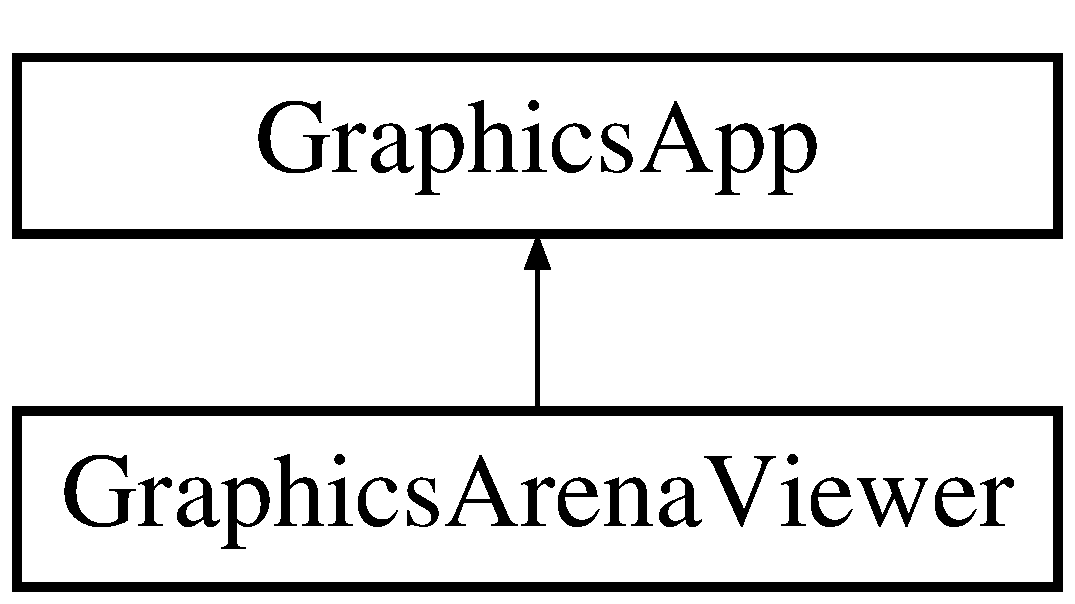
\includegraphics[height=2.000000cm]{class_graphics_arena_viewer}
\end{center}
\end{figure}
\subsection*{Public Member Functions}
\begin{DoxyCompactItemize}
\item 
\mbox{\hyperlink{class_graphics_arena_viewer_a869510833897508300da65b1eb0c5d09}{Graphics\+Arena\+Viewer}} (const struct \mbox{\hyperlink{structarena__params}{arena\+\_\+params}} $\ast$const params, \mbox{\hyperlink{class_arena}{Arena}} $\ast$arena, \mbox{\hyperlink{class_controller}{Controller}} $\ast$controller)
\begin{DoxyCompactList}\small\item\em Constructor. \end{DoxyCompactList}\item 
\mbox{\hyperlink{class_graphics_arena_viewer_a88cea02aab1550a7f315fbf4f3868109}{$\sim$\+Graphics\+Arena\+Viewer}} () override
\begin{DoxyCompactList}\small\item\em Destructor. \end{DoxyCompactList}\item 
void \mbox{\hyperlink{class_graphics_arena_viewer_aeec66666382aa0312574d70aa58de250}{Update\+Simulation}} (double dt) override
\begin{DoxyCompactList}\small\item\em Informs the \mbox{\hyperlink{class_arena}{Arena}} of the new time, so that it can update. \end{DoxyCompactList}\item 
void \mbox{\hyperlink{class_graphics_arena_viewer_a7cc65fd0e2e8c1f6138608e398c7c887}{On\+Playing\+Btn\+Pressed}} ()
\begin{DoxyCompactList}\small\item\em Handle the user pressing the pause button on the G\+UI. \end{DoxyCompactList}\item 
void \mbox{\hyperlink{class_graphics_arena_viewer_a74b5c524369a62ba419c89677c646d9e}{On\+Mouse\+Move}} (\mbox{\hyperlink{common_8h_a2e3484535ee610c8e19e9859563abe48}{\+\_\+\+\_\+unused}} const Point2 \&pos, \mbox{\hyperlink{common_8h_a2e3484535ee610c8e19e9859563abe48}{\+\_\+\+\_\+unused}} const Vector2 \&delta) override
\begin{DoxyCompactList}\small\item\em Called each time the mouse moves on the screen within the G\+UI window. \end{DoxyCompactList}\item 
void \mbox{\hyperlink{class_graphics_arena_viewer_adf2fb01c3ca8b1774f031d68616b288c}{On\+Left\+Mouse\+Down}} (\mbox{\hyperlink{common_8h_a2e3484535ee610c8e19e9859563abe48}{\+\_\+\+\_\+unused}} const Point2 \&pos) override
\begin{DoxyCompactList}\small\item\em Called each time the left mouse button is clicked. \end{DoxyCompactList}\item 
void \mbox{\hyperlink{class_graphics_arena_viewer_abe4f11ab9bfb6055280ddf2b671d7032}{On\+Left\+Mouse\+Up}} (\mbox{\hyperlink{common_8h_a2e3484535ee610c8e19e9859563abe48}{\+\_\+\+\_\+unused}} const Point2 \&pos) override
\begin{DoxyCompactList}\small\item\em Called each time the left mouse button is released. \end{DoxyCompactList}\item 
void \mbox{\hyperlink{class_graphics_arena_viewer_a178a9f09ff241d4dc032b6d0998cc9c6}{On\+Right\+Mouse\+Down}} (\mbox{\hyperlink{common_8h_a2e3484535ee610c8e19e9859563abe48}{\+\_\+\+\_\+unused}} const Point2 \&pos) override
\begin{DoxyCompactList}\small\item\em Called each time the right mouse button is clicked. \end{DoxyCompactList}\item 
void \mbox{\hyperlink{class_graphics_arena_viewer_a5dfa16dca83575e253b6d3ea344f8746}{On\+Right\+Mouse\+Up}} (\mbox{\hyperlink{common_8h_a2e3484535ee610c8e19e9859563abe48}{\+\_\+\+\_\+unused}} const Point2 \&pos) override
\begin{DoxyCompactList}\small\item\em Called each time the right mouse button is released. \end{DoxyCompactList}\item 
void \mbox{\hyperlink{class_graphics_arena_viewer_ab0001d4a3ebde2b1f5b4cb7770824726}{On\+Key\+Down}} (\mbox{\hyperlink{common_8h_a2e3484535ee610c8e19e9859563abe48}{\+\_\+\+\_\+unused}} const char $\ast$c, \mbox{\hyperlink{common_8h_a2e3484535ee610c8e19e9859563abe48}{\+\_\+\+\_\+unused}} int modifiers) override
\begin{DoxyCompactList}\small\item\em Called each time a character key is pressed. \end{DoxyCompactList}\item 
void \mbox{\hyperlink{class_graphics_arena_viewer_ac3e749f6a75bdd5b32d23c9c8913f9d8}{On\+Key\+Up}} (\mbox{\hyperlink{common_8h_a2e3484535ee610c8e19e9859563abe48}{\+\_\+\+\_\+unused}} const char $\ast$c, \mbox{\hyperlink{common_8h_a2e3484535ee610c8e19e9859563abe48}{\+\_\+\+\_\+unused}} int modifiers) override
\begin{DoxyCompactList}\small\item\em Called each time a character key is released. \end{DoxyCompactList}\item 
void \mbox{\hyperlink{class_graphics_arena_viewer_ab6ed6287ddf72f43f605482ce77b01a2}{On\+Special\+Key\+Down}} (int key, \mbox{\hyperlink{common_8h_a2e3484535ee610c8e19e9859563abe48}{\+\_\+\+\_\+unused}} int scancode, \mbox{\hyperlink{common_8h_a2e3484535ee610c8e19e9859563abe48}{\+\_\+\+\_\+unused}} int modifiers) override
\begin{DoxyCompactList}\small\item\em Called each time a special (non-\/alphabetic) key is pressed. \end{DoxyCompactList}\item 
void \mbox{\hyperlink{class_graphics_arena_viewer_a086e2e29e1a5745a8ee4f12996897b22}{On\+Special\+Key\+Up}} (\mbox{\hyperlink{common_8h_a2e3484535ee610c8e19e9859563abe48}{\+\_\+\+\_\+unused}} int key, \mbox{\hyperlink{common_8h_a2e3484535ee610c8e19e9859563abe48}{\+\_\+\+\_\+unused}} int scancode, \mbox{\hyperlink{common_8h_a2e3484535ee610c8e19e9859563abe48}{\+\_\+\+\_\+unused}} int modifiers) override
\begin{DoxyCompactList}\small\item\em Called each time a special (non-\/alphabetic) key is released. \end{DoxyCompactList}\item 
void \mbox{\hyperlink{class_graphics_arena_viewer_a7d59755e3f7674f382127fe135492eeb}{Draw\+Using\+Nano\+VG}} (N\+V\+Gcontext $\ast$ctx) override
\begin{DoxyCompactList}\small\item\em Draw the \mbox{\hyperlink{class_arena}{Arena}} with all of its entities using {\ttfamily nanogui}. \end{DoxyCompactList}\item 
\mbox{\Hypertarget{class_graphics_arena_viewer_af894508bfa039199c6ff7f1b5a7da158}\label{class_graphics_arena_viewer_af894508bfa039199c6ff7f1b5a7da158}} 
void \mbox{\hyperlink{class_graphics_arena_viewer_af894508bfa039199c6ff7f1b5a7da158}{Draw\+Using\+Open\+GL}} () override
\begin{DoxyCompactList}\small\item\em Draw using {\ttfamily Open\+GL}. This method is unimplemented, as currently we are doing all drawing with {\ttfamily nanovg} in this application, so it is empty. \end{DoxyCompactList}\item 
\mbox{\Hypertarget{class_graphics_arena_viewer_a289278f7b338fc60f983827d21b159ff}\label{class_graphics_arena_viewer_a289278f7b338fc60f983827d21b159ff}} 
\mbox{\hyperlink{class_graphics_arena_viewer}{Graphics\+Arena\+Viewer}} \& \mbox{\hyperlink{class_graphics_arena_viewer_a289278f7b338fc60f983827d21b159ff}{operator=}} (const \mbox{\hyperlink{class_graphics_arena_viewer}{Graphics\+Arena\+Viewer}} \&other)=delete
\begin{DoxyCompactList}\small\item\em Under certain circumstance, the compiler requires that the assignment operator is not defined. This {\ttfamily deletes} the default assignment operator. \end{DoxyCompactList}\item 
\mbox{\Hypertarget{class_graphics_arena_viewer_afa70b72e0769db0f3f41fe37bc540621}\label{class_graphics_arena_viewer_afa70b72e0769db0f3f41fe37bc540621}} 
\mbox{\hyperlink{class_graphics_arena_viewer_afa70b72e0769db0f3f41fe37bc540621}{Graphics\+Arena\+Viewer}} (const \mbox{\hyperlink{class_graphics_arena_viewer}{Graphics\+Arena\+Viewer}} \&other)=delete
\begin{DoxyCompactList}\small\item\em Under certain circumstance, the compiler requires that the copy constructor is not defined. This {\ttfamily deletes} the default copy constructor. \end{DoxyCompactList}\item 
\mbox{\Hypertarget{class_graphics_arena_viewer_a93fe946f83b4a2eb8d3acc056a564ebe}\label{class_graphics_arena_viewer_a93fe946f83b4a2eb8d3acc056a564ebe}} 
void {\bfseries Accept\+Communication} (Communication com)
\item 
\mbox{\Hypertarget{class_graphics_arena_viewer_a42639575b9092ea71946b88caf787530}\label{class_graphics_arena_viewer_a42639575b9092ea71946b88caf787530}} 
void {\bfseries On\+New\+Btn\+Pressed} ()
\item 
\mbox{\Hypertarget{class_graphics_arena_viewer_ae7eba0a3b3f7b2bddb40b2ddc6dfc694}\label{class_graphics_arena_viewer_ae7eba0a3b3f7b2bddb40b2ddc6dfc694}} 
void {\bfseries On\+Food\+Btn\+Pressed} ()
\item 
\mbox{\Hypertarget{class_graphics_arena_viewer_a16e84f4e03283928557f727d67f7839a}\label{class_graphics_arena_viewer_a16e84f4e03283928557f727d67f7839a}} 
void {\bfseries Set\+Arena} (\mbox{\hyperlink{class_arena}{Arena}} $\ast$newarena)
\end{DoxyCompactItemize}


\subsection{Detailed Description}
An application that uses the Min\+Gfx library to open up a window that includes a few buttons for controlling the simulation and can be used to draw circles and other computer graphics. 

After constructing a new \mbox{\hyperlink{class_graphics_arena_viewer}{Graphics\+Arena\+Viewer}}, call Run to start and run the application. Run will not return until the application window is closed. Example\+:


\begin{DoxyCode}
\DoxyCodeLine{\textcolor{keywordtype}{int} main(\textcolor{keywordtype}{int} argc, \textcolor{keywordtype}{char} **argv) \{}
\DoxyCodeLine{    RobotViewer *app = \textcolor{keyword}{new} RobotViewer();}
\DoxyCodeLine{    app->Run();}
\DoxyCodeLine{    \textcolor{keywordflow}{return} 0;}
\DoxyCodeLine{\}}
\end{DoxyCode}


While the window is open Update\+Simulation will be called repeatedly, once per frame. Fill this in to update your simulation or perform any other processing that should happen over time as the simulation progresses.

Fill in the {\ttfamily On$\ast$()} methods as desired to respond to user input events.

Fill in the {\ttfamily Draw$\ast$()} methods to draw graphics on the screen using either the {\ttfamily nanovg} library or raw {\ttfamily Open\+GL}. 

\subsection{Constructor \& Destructor Documentation}
\mbox{\Hypertarget{class_graphics_arena_viewer_a869510833897508300da65b1eb0c5d09}\label{class_graphics_arena_viewer_a869510833897508300da65b1eb0c5d09}} 
\index{Graphics\+Arena\+Viewer@{Graphics\+Arena\+Viewer}!Graphics\+Arena\+Viewer@{Graphics\+Arena\+Viewer}}
\index{Graphics\+Arena\+Viewer@{Graphics\+Arena\+Viewer}!Graphics\+Arena\+Viewer@{Graphics\+Arena\+Viewer}}
\subsubsection{\texorpdfstring{Graphics\+Arena\+Viewer()}{GraphicsArenaViewer()}}
{\footnotesize\ttfamily Graphics\+Arena\+Viewer\+::\+Graphics\+Arena\+Viewer (\begin{DoxyParamCaption}\item[{const struct \mbox{\hyperlink{structarena__params}{arena\+\_\+params}} $\ast$const}]{params,  }\item[{\mbox{\hyperlink{class_arena}{Arena}} $\ast$}]{arena,  }\item[{\mbox{\hyperlink{class_controller}{Controller}} $\ast$}]{controller }\end{DoxyParamCaption})\hspace{0.3cm}{\ttfamily [explicit]}}



Constructor. 


\begin{DoxyParams}{Parameters}
{\em params} & A \mbox{\hyperlink{structarena__params}{arena\+\_\+params}} passed down from \mbox{\hyperlink{main_8cc}{main.\+cc}} for the initialization of the \mbox{\hyperlink{class_arena}{Arena}} and the entities therein. \\
\hline
\end{DoxyParams}
\mbox{\Hypertarget{class_graphics_arena_viewer_a88cea02aab1550a7f315fbf4f3868109}\label{class_graphics_arena_viewer_a88cea02aab1550a7f315fbf4f3868109}} 
\index{Graphics\+Arena\+Viewer@{Graphics\+Arena\+Viewer}!````~Graphics\+Arena\+Viewer@{$\sim$\+Graphics\+Arena\+Viewer}}
\index{````~Graphics\+Arena\+Viewer@{$\sim$\+Graphics\+Arena\+Viewer}!Graphics\+Arena\+Viewer@{Graphics\+Arena\+Viewer}}
\subsubsection{\texorpdfstring{$\sim$\+Graphics\+Arena\+Viewer()}{~GraphicsArenaViewer()}}
{\footnotesize\ttfamily Graphics\+Arena\+Viewer\+::$\sim$\+Graphics\+Arena\+Viewer (\begin{DoxyParamCaption}{ }\end{DoxyParamCaption})\hspace{0.3cm}{\ttfamily [inline]}, {\ttfamily [override]}}



Destructor. 

{\ttfamily delete} the contained \mbox{\hyperlink{class_arena}{Arena}}. 

\subsection{Member Function Documentation}
\mbox{\Hypertarget{class_graphics_arena_viewer_a7d59755e3f7674f382127fe135492eeb}\label{class_graphics_arena_viewer_a7d59755e3f7674f382127fe135492eeb}} 
\index{Graphics\+Arena\+Viewer@{Graphics\+Arena\+Viewer}!Draw\+Using\+Nano\+VG@{Draw\+Using\+Nano\+VG}}
\index{Draw\+Using\+Nano\+VG@{Draw\+Using\+Nano\+VG}!Graphics\+Arena\+Viewer@{Graphics\+Arena\+Viewer}}
\subsubsection{\texorpdfstring{Draw\+Using\+Nano\+V\+G()}{DrawUsingNanoVG()}}
{\footnotesize\ttfamily void Graphics\+Arena\+Viewer\+::\+Draw\+Using\+Nano\+VG (\begin{DoxyParamCaption}\item[{N\+V\+Gcontext $\ast$}]{ctx }\end{DoxyParamCaption})\hspace{0.3cm}{\ttfamily [override]}}



Draw the \mbox{\hyperlink{class_arena}{Arena}} with all of its entities using {\ttfamily nanogui}. 

This is the primary driver for drawing all entities in the \mbox{\hyperlink{class_arena}{Arena}}. It is called at each iteration of {\ttfamily nanogui\+::mainloop()}.


\begin{DoxyParams}[1]{Parameters}
\mbox{\tt in}  & {\em ctx} & Context for nanogui. \\
\hline
\end{DoxyParams}
\mbox{\Hypertarget{class_graphics_arena_viewer_ab0001d4a3ebde2b1f5b4cb7770824726}\label{class_graphics_arena_viewer_ab0001d4a3ebde2b1f5b4cb7770824726}} 
\index{Graphics\+Arena\+Viewer@{Graphics\+Arena\+Viewer}!On\+Key\+Down@{On\+Key\+Down}}
\index{On\+Key\+Down@{On\+Key\+Down}!Graphics\+Arena\+Viewer@{Graphics\+Arena\+Viewer}}
\subsubsection{\texorpdfstring{On\+Key\+Down()}{OnKeyDown()}}
{\footnotesize\ttfamily void Graphics\+Arena\+Viewer\+::\+On\+Key\+Down (\begin{DoxyParamCaption}\item[{\mbox{\hyperlink{common_8h_a2e3484535ee610c8e19e9859563abe48}{\+\_\+\+\_\+unused}} const char $\ast$}]{c,  }\item[{\mbox{\hyperlink{common_8h_a2e3484535ee610c8e19e9859563abe48}{\+\_\+\+\_\+unused}} int}]{modifiers }\end{DoxyParamCaption})\hspace{0.3cm}{\ttfamily [inline]}, {\ttfamily [override]}}



Called each time a character key is pressed. 


\begin{DoxyParams}[1]{Parameters}
\mbox{\tt in}  & {\em c} & Character representing a key that was pressed. \\
\hline
\mbox{\tt in}  & {\em modifiers} & Any modifier keys that were also pressed. \\
\hline
\end{DoxyParams}
\mbox{\Hypertarget{class_graphics_arena_viewer_ac3e749f6a75bdd5b32d23c9c8913f9d8}\label{class_graphics_arena_viewer_ac3e749f6a75bdd5b32d23c9c8913f9d8}} 
\index{Graphics\+Arena\+Viewer@{Graphics\+Arena\+Viewer}!On\+Key\+Up@{On\+Key\+Up}}
\index{On\+Key\+Up@{On\+Key\+Up}!Graphics\+Arena\+Viewer@{Graphics\+Arena\+Viewer}}
\subsubsection{\texorpdfstring{On\+Key\+Up()}{OnKeyUp()}}
{\footnotesize\ttfamily void Graphics\+Arena\+Viewer\+::\+On\+Key\+Up (\begin{DoxyParamCaption}\item[{\mbox{\hyperlink{common_8h_a2e3484535ee610c8e19e9859563abe48}{\+\_\+\+\_\+unused}} const char $\ast$}]{c,  }\item[{\mbox{\hyperlink{common_8h_a2e3484535ee610c8e19e9859563abe48}{\+\_\+\+\_\+unused}} int}]{modifiers }\end{DoxyParamCaption})\hspace{0.3cm}{\ttfamily [inline]}, {\ttfamily [override]}}



Called each time a character key is released. 


\begin{DoxyParams}[1]{Parameters}
\mbox{\tt in}  & {\em c} & Character representing a key that was released. \\
\hline
\mbox{\tt in}  & {\em modifiers} & Any modifier keys that were held with the key. \\
\hline
\end{DoxyParams}
\mbox{\Hypertarget{class_graphics_arena_viewer_adf2fb01c3ca8b1774f031d68616b288c}\label{class_graphics_arena_viewer_adf2fb01c3ca8b1774f031d68616b288c}} 
\index{Graphics\+Arena\+Viewer@{Graphics\+Arena\+Viewer}!On\+Left\+Mouse\+Down@{On\+Left\+Mouse\+Down}}
\index{On\+Left\+Mouse\+Down@{On\+Left\+Mouse\+Down}!Graphics\+Arena\+Viewer@{Graphics\+Arena\+Viewer}}
\subsubsection{\texorpdfstring{On\+Left\+Mouse\+Down()}{OnLeftMouseDown()}}
{\footnotesize\ttfamily void Graphics\+Arena\+Viewer\+::\+On\+Left\+Mouse\+Down (\begin{DoxyParamCaption}\item[{\mbox{\hyperlink{common_8h_a2e3484535ee610c8e19e9859563abe48}{\+\_\+\+\_\+unused}} const Point2 \&}]{pos }\end{DoxyParamCaption})\hspace{0.3cm}{\ttfamily [inline]}, {\ttfamily [override]}}



Called each time the left mouse button is clicked. 

Origin is at the lower left of the window. This function is a stub.


\begin{DoxyParams}[1]{Parameters}
\mbox{\tt in}  & {\em pos} & The position of the release. \\
\hline
\end{DoxyParams}
\mbox{\Hypertarget{class_graphics_arena_viewer_abe4f11ab9bfb6055280ddf2b671d7032}\label{class_graphics_arena_viewer_abe4f11ab9bfb6055280ddf2b671d7032}} 
\index{Graphics\+Arena\+Viewer@{Graphics\+Arena\+Viewer}!On\+Left\+Mouse\+Up@{On\+Left\+Mouse\+Up}}
\index{On\+Left\+Mouse\+Up@{On\+Left\+Mouse\+Up}!Graphics\+Arena\+Viewer@{Graphics\+Arena\+Viewer}}
\subsubsection{\texorpdfstring{On\+Left\+Mouse\+Up()}{OnLeftMouseUp()}}
{\footnotesize\ttfamily void Graphics\+Arena\+Viewer\+::\+On\+Left\+Mouse\+Up (\begin{DoxyParamCaption}\item[{\mbox{\hyperlink{common_8h_a2e3484535ee610c8e19e9859563abe48}{\+\_\+\+\_\+unused}} const Point2 \&}]{pos }\end{DoxyParamCaption})\hspace{0.3cm}{\ttfamily [inline]}, {\ttfamily [override]}}



Called each time the left mouse button is released. 

Origin is at the lower left of the window. This function is a stub.


\begin{DoxyParams}[1]{Parameters}
\mbox{\tt in}  & {\em pos} & The position of the release. \\
\hline
\end{DoxyParams}
\mbox{\Hypertarget{class_graphics_arena_viewer_a74b5c524369a62ba419c89677c646d9e}\label{class_graphics_arena_viewer_a74b5c524369a62ba419c89677c646d9e}} 
\index{Graphics\+Arena\+Viewer@{Graphics\+Arena\+Viewer}!On\+Mouse\+Move@{On\+Mouse\+Move}}
\index{On\+Mouse\+Move@{On\+Mouse\+Move}!Graphics\+Arena\+Viewer@{Graphics\+Arena\+Viewer}}
\subsubsection{\texorpdfstring{On\+Mouse\+Move()}{OnMouseMove()}}
{\footnotesize\ttfamily void Graphics\+Arena\+Viewer\+::\+On\+Mouse\+Move (\begin{DoxyParamCaption}\item[{\mbox{\hyperlink{common_8h_a2e3484535ee610c8e19e9859563abe48}{\+\_\+\+\_\+unused}} const Point2 \&}]{pos,  }\item[{\mbox{\hyperlink{common_8h_a2e3484535ee610c8e19e9859563abe48}{\+\_\+\+\_\+unused}} const Vector2 \&}]{delta }\end{DoxyParamCaption})\hspace{0.3cm}{\ttfamily [inline]}, {\ttfamily [override]}}



Called each time the mouse moves on the screen within the G\+UI window. 

Origin is at the lower left of the window. This function is a stub.


\begin{DoxyParams}[1]{Parameters}
\mbox{\tt in}  & {\em pos} & The position of the release. \\
\hline
\mbox{\tt in}  & {\em delta} & How far the mouse has moved. \\
\hline
\end{DoxyParams}
\mbox{\Hypertarget{class_graphics_arena_viewer_a7cc65fd0e2e8c1f6138608e398c7c887}\label{class_graphics_arena_viewer_a7cc65fd0e2e8c1f6138608e398c7c887}} 
\index{Graphics\+Arena\+Viewer@{Graphics\+Arena\+Viewer}!On\+Playing\+Btn\+Pressed@{On\+Playing\+Btn\+Pressed}}
\index{On\+Playing\+Btn\+Pressed@{On\+Playing\+Btn\+Pressed}!Graphics\+Arena\+Viewer@{Graphics\+Arena\+Viewer}}
\subsubsection{\texorpdfstring{On\+Playing\+Btn\+Pressed()}{OnPlayingBtnPressed()}}
{\footnotesize\ttfamily void Graphics\+Arena\+Viewer\+::\+On\+Playing\+Btn\+Pressed (\begin{DoxyParamCaption}{ }\end{DoxyParamCaption})}



Handle the user pressing the pause button on the G\+UI. 

This will freeze the graphics--no update, until the pause button is pressed again. \mbox{\Hypertarget{class_graphics_arena_viewer_a178a9f09ff241d4dc032b6d0998cc9c6}\label{class_graphics_arena_viewer_a178a9f09ff241d4dc032b6d0998cc9c6}} 
\index{Graphics\+Arena\+Viewer@{Graphics\+Arena\+Viewer}!On\+Right\+Mouse\+Down@{On\+Right\+Mouse\+Down}}
\index{On\+Right\+Mouse\+Down@{On\+Right\+Mouse\+Down}!Graphics\+Arena\+Viewer@{Graphics\+Arena\+Viewer}}
\subsubsection{\texorpdfstring{On\+Right\+Mouse\+Down()}{OnRightMouseDown()}}
{\footnotesize\ttfamily void Graphics\+Arena\+Viewer\+::\+On\+Right\+Mouse\+Down (\begin{DoxyParamCaption}\item[{\mbox{\hyperlink{common_8h_a2e3484535ee610c8e19e9859563abe48}{\+\_\+\+\_\+unused}} const Point2 \&}]{pos }\end{DoxyParamCaption})\hspace{0.3cm}{\ttfamily [inline]}, {\ttfamily [override]}}



Called each time the right mouse button is clicked. 

Origin is at the lower left of the window. This function is a stub.


\begin{DoxyParams}[1]{Parameters}
\mbox{\tt in}  & {\em pos} & The position of the release. \\
\hline
\end{DoxyParams}
\mbox{\Hypertarget{class_graphics_arena_viewer_a5dfa16dca83575e253b6d3ea344f8746}\label{class_graphics_arena_viewer_a5dfa16dca83575e253b6d3ea344f8746}} 
\index{Graphics\+Arena\+Viewer@{Graphics\+Arena\+Viewer}!On\+Right\+Mouse\+Up@{On\+Right\+Mouse\+Up}}
\index{On\+Right\+Mouse\+Up@{On\+Right\+Mouse\+Up}!Graphics\+Arena\+Viewer@{Graphics\+Arena\+Viewer}}
\subsubsection{\texorpdfstring{On\+Right\+Mouse\+Up()}{OnRightMouseUp()}}
{\footnotesize\ttfamily void Graphics\+Arena\+Viewer\+::\+On\+Right\+Mouse\+Up (\begin{DoxyParamCaption}\item[{\mbox{\hyperlink{common_8h_a2e3484535ee610c8e19e9859563abe48}{\+\_\+\+\_\+unused}} const Point2 \&}]{pos }\end{DoxyParamCaption})\hspace{0.3cm}{\ttfamily [inline]}, {\ttfamily [override]}}



Called each time the right mouse button is released. 

Origin is at the lower left of the window. This function is a stub.


\begin{DoxyParams}[1]{Parameters}
\mbox{\tt in}  & {\em pos} & The position of the release. \\
\hline
\end{DoxyParams}
\mbox{\Hypertarget{class_graphics_arena_viewer_ab6ed6287ddf72f43f605482ce77b01a2}\label{class_graphics_arena_viewer_ab6ed6287ddf72f43f605482ce77b01a2}} 
\index{Graphics\+Arena\+Viewer@{Graphics\+Arena\+Viewer}!On\+Special\+Key\+Down@{On\+Special\+Key\+Down}}
\index{On\+Special\+Key\+Down@{On\+Special\+Key\+Down}!Graphics\+Arena\+Viewer@{Graphics\+Arena\+Viewer}}
\subsubsection{\texorpdfstring{On\+Special\+Key\+Down()}{OnSpecialKeyDown()}}
{\footnotesize\ttfamily void Graphics\+Arena\+Viewer\+::\+On\+Special\+Key\+Down (\begin{DoxyParamCaption}\item[{int}]{key,  }\item[{\mbox{\hyperlink{common_8h_a2e3484535ee610c8e19e9859563abe48}{\+\_\+\+\_\+unused}} int}]{scancode,  }\item[{\mbox{\hyperlink{common_8h_a2e3484535ee610c8e19e9859563abe48}{\+\_\+\+\_\+unused}} int}]{modifiers }\end{DoxyParamCaption})\hspace{0.3cm}{\ttfamily [override]}}



Called each time a special (non-\/alphabetic) key is pressed. 


\begin{DoxyParams}[1]{Parameters}
\mbox{\tt in}  & {\em key} & The key that was pressed. \\
\hline
\mbox{\tt in}  & {\em scancode} & The scancode corresponding to the key. \\
\hline
\mbox{\tt in}  & {\em modifiers} & Any modifier keys that were also pressed.\\
\hline
\end{DoxyParams}
On\+Special\+Key\+Down is called when the user presses down on one of the special keys (e.\+g. the arrow keys).\+: Check for arrow key presses using G\+L\+FW macros, then convert to appropriate enum Communication and relay to controller \mbox{\Hypertarget{class_graphics_arena_viewer_a086e2e29e1a5745a8ee4f12996897b22}\label{class_graphics_arena_viewer_a086e2e29e1a5745a8ee4f12996897b22}} 
\index{Graphics\+Arena\+Viewer@{Graphics\+Arena\+Viewer}!On\+Special\+Key\+Up@{On\+Special\+Key\+Up}}
\index{On\+Special\+Key\+Up@{On\+Special\+Key\+Up}!Graphics\+Arena\+Viewer@{Graphics\+Arena\+Viewer}}
\subsubsection{\texorpdfstring{On\+Special\+Key\+Up()}{OnSpecialKeyUp()}}
{\footnotesize\ttfamily void Graphics\+Arena\+Viewer\+::\+On\+Special\+Key\+Up (\begin{DoxyParamCaption}\item[{\mbox{\hyperlink{common_8h_a2e3484535ee610c8e19e9859563abe48}{\+\_\+\+\_\+unused}} int}]{key,  }\item[{\mbox{\hyperlink{common_8h_a2e3484535ee610c8e19e9859563abe48}{\+\_\+\+\_\+unused}} int}]{scancode,  }\item[{\mbox{\hyperlink{common_8h_a2e3484535ee610c8e19e9859563abe48}{\+\_\+\+\_\+unused}} int}]{modifiers }\end{DoxyParamCaption})\hspace{0.3cm}{\ttfamily [inline]}, {\ttfamily [override]}}



Called each time a special (non-\/alphabetic) key is released. 


\begin{DoxyParams}[1]{Parameters}
\mbox{\tt in}  & {\em key} & The key that was released. \\
\hline
\mbox{\tt in}  & {\em scancode} & The scancode corresponding to the key. \\
\hline
\mbox{\tt in}  & {\em modifiers} & Any modifier keys that were also pressed. \\
\hline
\end{DoxyParams}
\mbox{\Hypertarget{class_graphics_arena_viewer_aeec66666382aa0312574d70aa58de250}\label{class_graphics_arena_viewer_aeec66666382aa0312574d70aa58de250}} 
\index{Graphics\+Arena\+Viewer@{Graphics\+Arena\+Viewer}!Update\+Simulation@{Update\+Simulation}}
\index{Update\+Simulation@{Update\+Simulation}!Graphics\+Arena\+Viewer@{Graphics\+Arena\+Viewer}}
\subsubsection{\texorpdfstring{Update\+Simulation()}{UpdateSimulation()}}
{\footnotesize\ttfamily void Graphics\+Arena\+Viewer\+::\+Update\+Simulation (\begin{DoxyParamCaption}\item[{double}]{dt }\end{DoxyParamCaption})\hspace{0.3cm}{\ttfamily [override]}}



Informs the \mbox{\hyperlink{class_arena}{Arena}} of the new time, so that it can update. 


\begin{DoxyParams}{Parameters}
{\em dt} & The new timestep. \\
\hline
\end{DoxyParams}


The documentation for this class was generated from the following files\+:\begin{DoxyCompactItemize}
\item 
src/\mbox{\hyperlink{graphics__arena__viewer_8h}{graphics\+\_\+arena\+\_\+viewer.\+h}}\item 
src/\mbox{\hyperlink{graphics__arena__viewer_8cc}{graphics\+\_\+arena\+\_\+viewer.\+cc}}\end{DoxyCompactItemize}

\hypertarget{class_light}{}\section{Light Class Reference}
\label{class_light}\index{Light@{Light}}


Class representing an immobile obstacle within the \mbox{\hyperlink{class_arena}{Arena}}.  




{\ttfamily \#include $<$light.\+h$>$}

Inheritance diagram for Light\+:\begin{figure}[H]
\begin{center}
\leavevmode
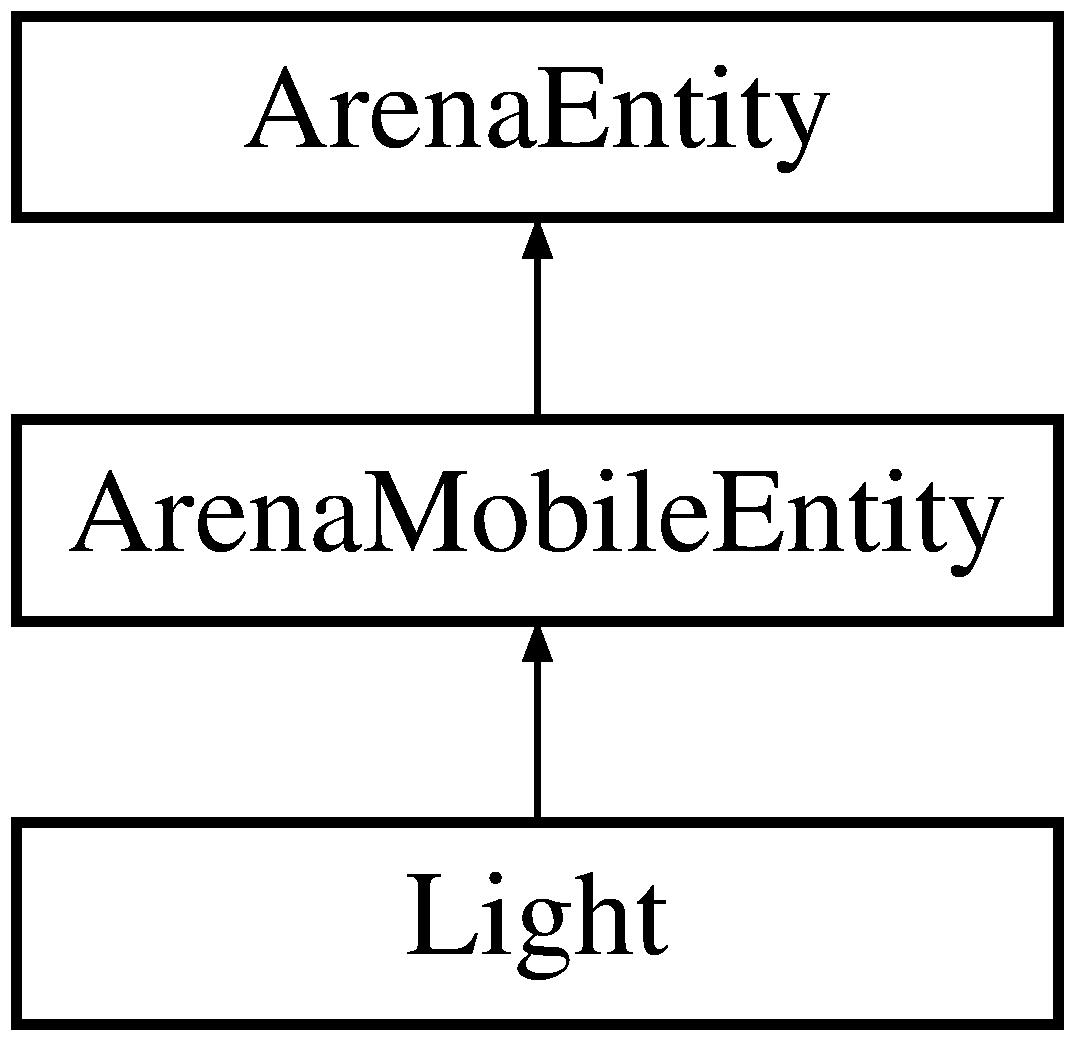
\includegraphics[height=3.000000cm]{class_light}
\end{center}
\end{figure}
\subsection*{Public Member Functions}
\begin{DoxyCompactItemize}
\item 
\mbox{\Hypertarget{class_light_aeb5df09a25a32f19fdffa761268ba24f}\label{class_light_aeb5df09a25a32f19fdffa761268ba24f}} 
\mbox{\hyperlink{class_light_aeb5df09a25a32f19fdffa761268ba24f}{Light}} ()
\begin{DoxyCompactList}\small\item\em Constructor. \end{DoxyCompactList}\item 
\mbox{\Hypertarget{class_light_a61485eb0684868b503e1b96e6a3206c3}\label{class_light_a61485eb0684868b503e1b96e6a3206c3}} 
void \mbox{\hyperlink{class_light_a61485eb0684868b503e1b96e6a3206c3}{Reset}} () override
\begin{DoxyCompactList}\small\item\em Reset entity to a newly constructed state. \end{DoxyCompactList}\item 
\mbox{\Hypertarget{class_light_a49b2e32cf8173353ac4689fdadbb95d5}\label{class_light_a49b2e32cf8173353ac4689fdadbb95d5}} 
std\+::string \mbox{\hyperlink{class_light_a49b2e32cf8173353ac4689fdadbb95d5}{get\+\_\+name}} () const override
\begin{DoxyCompactList}\small\item\em Get the name of the Obstacle for visualization purposes, and to aid in debugging. \end{DoxyCompactList}\item 
\mbox{\Hypertarget{class_light_a97934eec7489f9b072534f5e30a2d90d}\label{class_light_a97934eec7489f9b072534f5e30a2d90d}} 
void {\bfseries Timestep\+Update} (unsigned int dt) override
\item 
\mbox{\Hypertarget{class_light_ad8f77c9857b26273d913a18be1311a11}\label{class_light_ad8f77c9857b26273d913a18be1311a11}} 
void \mbox{\hyperlink{class_light_ad8f77c9857b26273d913a18be1311a11}{Handle\+Collision}} (Entity\+Type object\+\_\+type, \mbox{\hyperlink{class_arena_entity}{Arena\+Entity}} $\ast$object=N\+U\+LL) override
\begin{DoxyCompactList}\small\item\em Handles the collision by setting the sensor to activated. \end{DoxyCompactList}\item 
\mbox{\Hypertarget{class_light_a3a8b57cc040b0ab220cbc89d947fd2ab}\label{class_light_a3a8b57cc040b0ab220cbc89d947fd2ab}} 
void \mbox{\hyperlink{class_light_a3a8b57cc040b0ab220cbc89d947fd2ab}{Increase\+Speed}} ()
\begin{DoxyCompactList}\small\item\em Command that comes from the controller, then is passed to handler. \end{DoxyCompactList}\item 
\mbox{\Hypertarget{class_light_ade825fe740b39f80aa934588e29d12f9}\label{class_light_ade825fe740b39f80aa934588e29d12f9}} 
void \mbox{\hyperlink{class_light_ade825fe740b39f80aa934588e29d12f9}{Decrease\+Speed}} ()
\begin{DoxyCompactList}\small\item\em Command that comes from the controller, then is passed to handler. \end{DoxyCompactList}\item 
\mbox{\Hypertarget{class_light_a3d96e80148c96e450007da8358613187}\label{class_light_a3d96e80148c96e450007da8358613187}} 
void \mbox{\hyperlink{class_light_a3d96e80148c96e450007da8358613187}{Turn\+Right}} ()
\begin{DoxyCompactList}\small\item\em Command that comes from the controller, then is passed to handler. \end{DoxyCompactList}\item 
\mbox{\Hypertarget{class_light_a571db6b9e9478fbced0cf9212fa44fb4}\label{class_light_a571db6b9e9478fbced0cf9212fa44fb4}} 
void \mbox{\hyperlink{class_light_a571db6b9e9478fbced0cf9212fa44fb4}{Turn\+Left}} ()
\begin{DoxyCompactList}\small\item\em Command that comes from the controller, then is passed to handler. \end{DoxyCompactList}\item 
\mbox{\Hypertarget{class_light_a056a03454affa4a64dfd6188e5cf8f4d}\label{class_light_a056a03454affa4a64dfd6188e5cf8f4d}} 
\mbox{\hyperlink{class_motion_handler}{Motion\+Handler}} \& {\bfseries get\+\_\+motion\+\_\+handler} ()
\item 
\mbox{\Hypertarget{class_light_af8a67e1e3d3e6b21c169cfd6bdaa8ab2}\label{class_light_af8a67e1e3d3e6b21c169cfd6bdaa8ab2}} 
\mbox{\hyperlink{class_motion_behavior_differential}{Motion\+Behavior\+Differential}} {\bfseries get\+\_\+motion\+\_\+behavior} ()
\item 
\mbox{\Hypertarget{class_light_ae7c1f02a58289be086e15e06df29a8dc}\label{class_light_ae7c1f02a58289be086e15e06df29a8dc}} 
int {\bfseries get\+\_\+state} ()
\item 
\mbox{\Hypertarget{class_light_a1296a373c45d54eb68a16b648d100c6c}\label{class_light_a1296a373c45d54eb68a16b648d100c6c}} 
void {\bfseries set\+\_\+state} (int state)
\end{DoxyCompactItemize}
\subsection*{Additional Inherited Members}


\subsection{Detailed Description}
Class representing an immobile obstacle within the \mbox{\hyperlink{class_arena}{Arena}}. 

Since obstacles are immobile, the Obstacle class is very simple. 

The documentation for this class was generated from the following files\+:\begin{DoxyCompactItemize}
\item 
src/light.\+h\item 
src/light.\+cc\end{DoxyCompactItemize}

\hypertarget{class_light_sensor}{}\section{Light\+Sensor Class Reference}
\label{class_light_sensor}\index{Light\+Sensor@{Light\+Sensor}}


Class representing a \mbox{\hyperlink{class_light}{Light}} sensor.  




{\ttfamily \#include $<$light\+\_\+sensor.\+h$>$}

Inheritance diagram for Light\+Sensor\+:\begin{figure}[H]
\begin{center}
\leavevmode
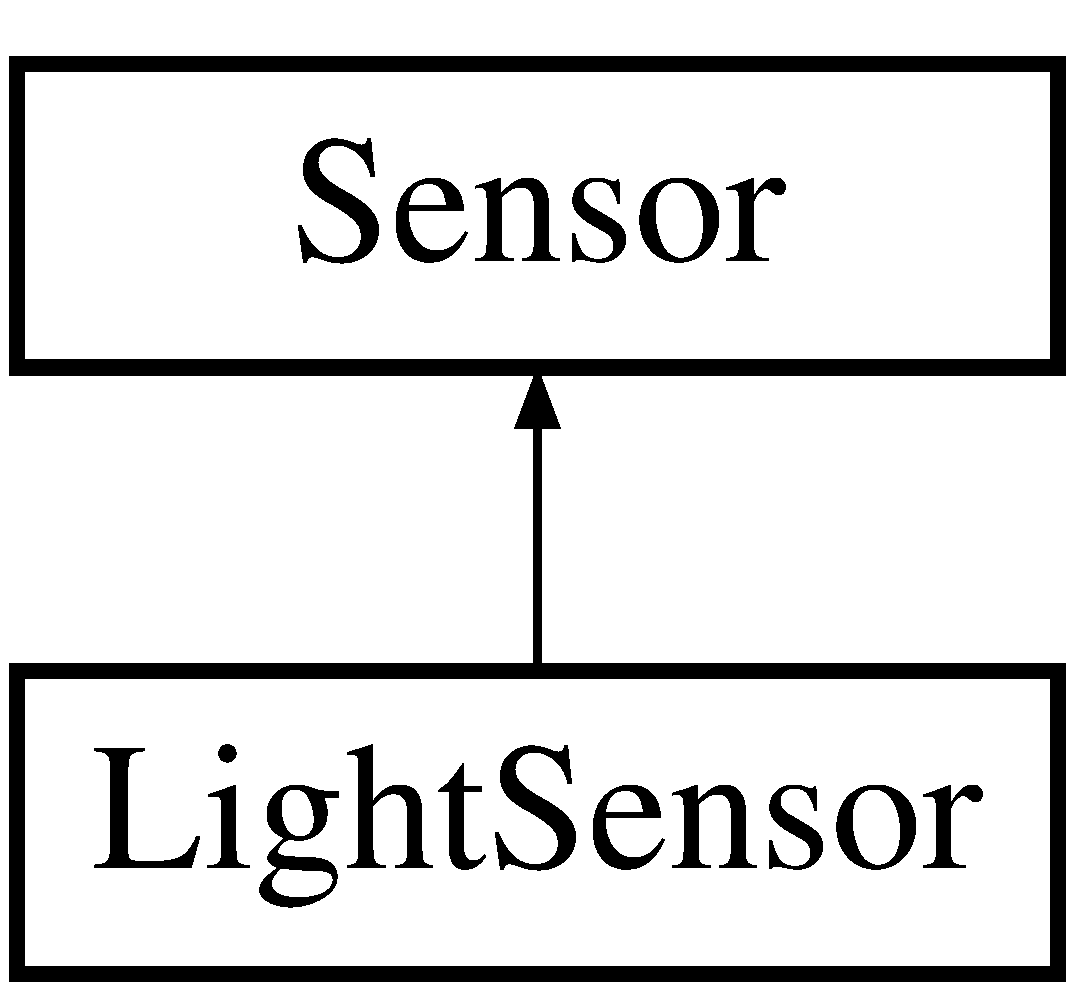
\includegraphics[height=2.000000cm]{class_light_sensor}
\end{center}
\end{figure}
\subsection*{Public Member Functions}
\begin{DoxyCompactItemize}
\item 
\mbox{\Hypertarget{class_light_sensor_af5ec9461f434abd6558e0e63d60e8912}\label{class_light_sensor_af5ec9461f434abd6558e0e63d60e8912}} 
{\bfseries Light\+Sensor} (int xpos, int ypos)
\end{DoxyCompactItemize}


\subsection{Detailed Description}
Class representing a \mbox{\hyperlink{class_light}{Light}} sensor. 

This is a \mbox{\hyperlink{class_light}{Light}} sensor class that takes in the the position of the entity being sensed it then calculates the reading based on the position of that entity and its own position which it holds. This class inherits from base sensor and most of the work is done in that class. Sensors are fed readings and return them when prompted. 

The documentation for this class was generated from the following file\+:\begin{DoxyCompactItemize}
\item 
src/light\+\_\+sensor.\+h\end{DoxyCompactItemize}

\hypertarget{class_motion_behavior}{}\section{Motion\+Behavior Class Reference}
\label{class_motion_behavior}\index{Motion\+Behavior@{Motion\+Behavior}}


Class managing an \mbox{\hyperlink{class_arena_mobile_entity}{Arena\+Mobile\+Entity}}\textquotesingle{}s position.  




{\ttfamily \#include $<$motion\+\_\+behavior.\+h$>$}

Inheritance diagram for Motion\+Behavior\+:\begin{figure}[H]
\begin{center}
\leavevmode
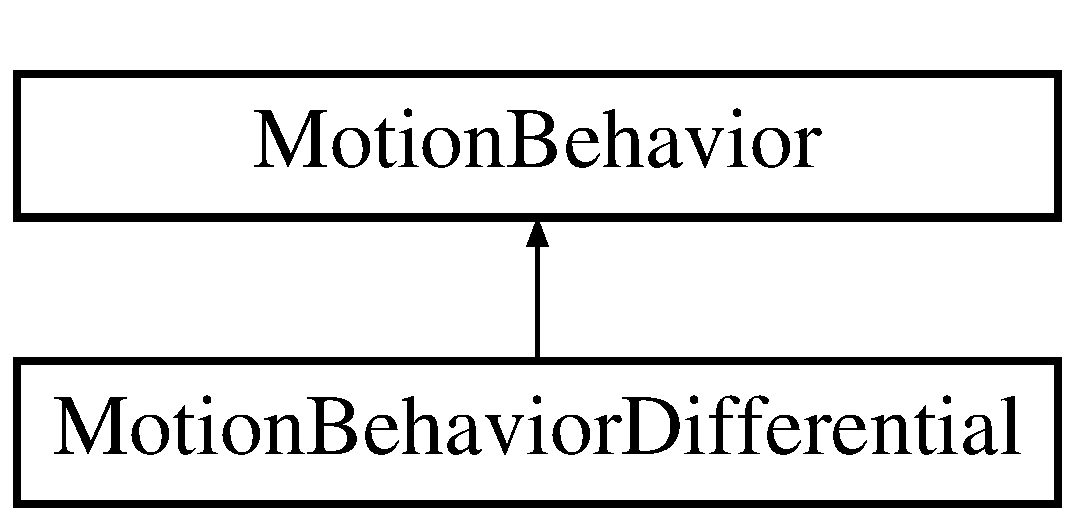
\includegraphics[height=2.000000cm]{class_motion_behavior}
\end{center}
\end{figure}
\subsection*{Public Member Functions}
\begin{DoxyCompactItemize}
\item 
\mbox{\Hypertarget{class_motion_behavior_aa2d5f7d563f4fdb5702edb8367eaa6e7}\label{class_motion_behavior_aa2d5f7d563f4fdb5702edb8367eaa6e7}} 
\mbox{\hyperlink{class_motion_behavior_aa2d5f7d563f4fdb5702edb8367eaa6e7}{Motion\+Behavior}} (\mbox{\hyperlink{class_arena_mobile_entity}{Arena\+Mobile\+Entity}} $\ast$ent)
\begin{DoxyCompactList}\small\item\em Default constructor. \end{DoxyCompactList}\item 
\mbox{\Hypertarget{class_motion_behavior_a5fe8e8a49e8cb34519a34ca652a23143}\label{class_motion_behavior_a5fe8e8a49e8cb34519a34ca652a23143}} 
{\bfseries Motion\+Behavior} (const \mbox{\hyperlink{class_motion_behavior}{Motion\+Behavior}} \&other)=default
\item 
\mbox{\Hypertarget{class_motion_behavior_a227057c1862c64bbc609705205473abc}\label{class_motion_behavior_a227057c1862c64bbc609705205473abc}} 
\mbox{\hyperlink{class_motion_behavior}{Motion\+Behavior}} \& {\bfseries operator=} (const \mbox{\hyperlink{class_motion_behavior}{Motion\+Behavior}} \&other)=default
\item 
virtual void \mbox{\hyperlink{class_motion_behavior_a804f440bb7f03f19abec79a1ab671494}{Update\+Pose}} (double dt, \mbox{\hyperlink{struct_wheel_velocity}{Wheel\+Velocity}} vel=\mbox{\hyperlink{struct_wheel_velocity}{Wheel\+Velocity}}())
\begin{DoxyCompactList}\small\item\em Update the position (and possibly orientation) for an \mbox{\hyperlink{class_arena_mobile_entity}{Arena\+Mobile\+Entity}}, foodd on its current position and velocity. \end{DoxyCompactList}\item 
\mbox{\Hypertarget{class_motion_behavior_a1daf82b16d312ba6f5f71178e7fafa79}\label{class_motion_behavior_a1daf82b16d312ba6f5f71178e7fafa79}} 
\mbox{\hyperlink{class_arena_mobile_entity}{Arena\+Mobile\+Entity}} $\ast$ \mbox{\hyperlink{class_motion_behavior_a1daf82b16d312ba6f5f71178e7fafa79}{get\+\_\+entity}} ()
\begin{DoxyCompactList}\small\item\em Getter of entity in which this class was created. \end{DoxyCompactList}\end{DoxyCompactItemize}
\subsection*{Protected Attributes}
\begin{DoxyCompactItemize}
\item 
\mbox{\Hypertarget{class_motion_behavior_a9254cf197657a2a52d89dbc01da31b8f}\label{class_motion_behavior_a9254cf197657a2a52d89dbc01da31b8f}} 
\mbox{\hyperlink{class_arena_mobile_entity}{Arena\+Mobile\+Entity}} $\ast$ {\bfseries entity\+\_\+}
\end{DoxyCompactItemize}


\subsection{Detailed Description}
Class managing an \mbox{\hyperlink{class_arena_mobile_entity}{Arena\+Mobile\+Entity}}\textquotesingle{}s position. 

Update the position foodd on the current speed and position. This is simple, but the framework allows for more sophisticated models of motion in which each wheel has different speeds. 

\subsection{Member Function Documentation}
\mbox{\Hypertarget{class_motion_behavior_a804f440bb7f03f19abec79a1ab671494}\label{class_motion_behavior_a804f440bb7f03f19abec79a1ab671494}} 
\index{Motion\+Behavior@{Motion\+Behavior}!Update\+Pose@{Update\+Pose}}
\index{Update\+Pose@{Update\+Pose}!Motion\+Behavior@{Motion\+Behavior}}
\subsubsection{\texorpdfstring{Update\+Pose()}{UpdatePose()}}
{\footnotesize\ttfamily void Motion\+Behavior\+::\+Update\+Pose (\begin{DoxyParamCaption}\item[{double}]{dt,  }\item[{\mbox{\hyperlink{struct_wheel_velocity}{Wheel\+Velocity}}}]{vel = {\ttfamily \mbox{\hyperlink{struct_wheel_velocity}{Wheel\+Velocity}}()} }\end{DoxyParamCaption})\hspace{0.3cm}{\ttfamily [virtual]}}



Update the position (and possibly orientation) for an \mbox{\hyperlink{class_arena_mobile_entity}{Arena\+Mobile\+Entity}}, foodd on its current position and velocity. 


\begin{DoxyParams}[1]{Parameters}
\mbox{\tt in}  & {\em dt} & \# of timesteps elapsed since the last update. \\
\hline
\mbox{\tt in}  & {\em vel} & \mbox{\hyperlink{struct_wheel_velocity}{Wheel\+Velocity}} stored within the motion handler \\
\hline
\end{DoxyParams}


Reimplemented in \mbox{\hyperlink{class_motion_behavior_differential_a929c3a05aa2072acf2a508109b1259ef}{Motion\+Behavior\+Differential}}.



The documentation for this class was generated from the following files\+:\begin{DoxyCompactItemize}
\item 
src/\mbox{\hyperlink{motion__behavior_8h}{motion\+\_\+behavior.\+h}}\item 
src/\mbox{\hyperlink{motion__behavior_8cc}{motion\+\_\+behavior.\+cc}}\end{DoxyCompactItemize}

\hypertarget{class_motion_behavior_differential}{}\section{Motion\+Behavior\+Differential Class Reference}
\label{class_motion_behavior_differential}\index{Motion\+Behavior\+Differential@{Motion\+Behavior\+Differential}}


A simple model of differential drive kinematics foodd on the notes here\+: $\sim$https\+://chess.eecs.\+berkeley.\+edu/eecs149/documentation/differential\+Drive.\+pdf$\sim$.  




{\ttfamily \#include $<$motion\+\_\+behavior\+\_\+differential.\+h$>$}

Inheritance diagram for Motion\+Behavior\+Differential\+:\begin{figure}[H]
\begin{center}
\leavevmode
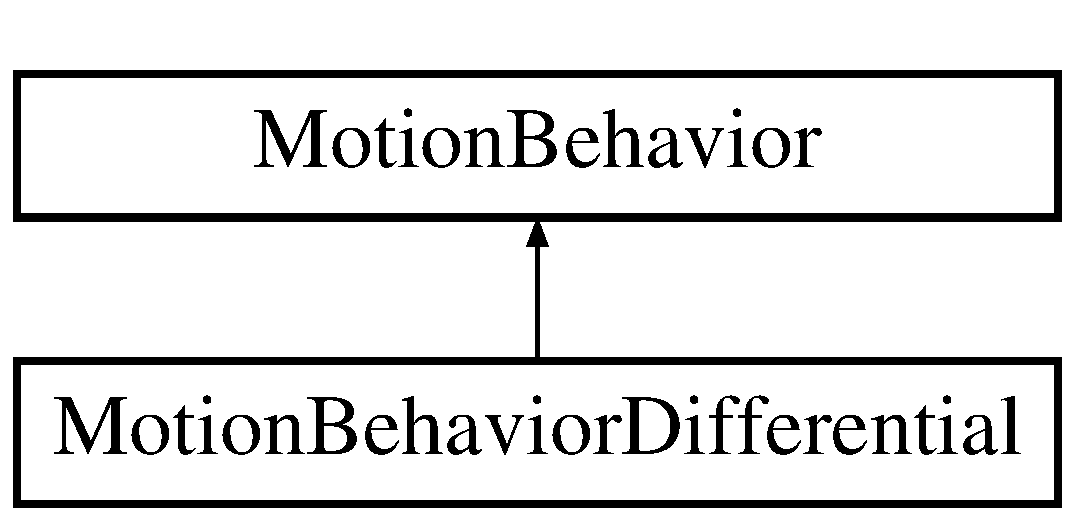
\includegraphics[height=2.000000cm]{class_motion_behavior_differential}
\end{center}
\end{figure}
\subsection*{Public Member Functions}
\begin{DoxyCompactItemize}
\item 
\mbox{\Hypertarget{class_motion_behavior_differential_a8815791ac85212945862454560279d28}\label{class_motion_behavior_differential_a8815791ac85212945862454560279d28}} 
{\bfseries Motion\+Behavior\+Differential} (\mbox{\hyperlink{class_arena_mobile_entity}{Arena\+Mobile\+Entity}} $\ast$entity)
\item 
\mbox{\Hypertarget{class_motion_behavior_differential_aeaa480aac3de205e1d177c4b4ad73ed6}\label{class_motion_behavior_differential_aeaa480aac3de205e1d177c4b4ad73ed6}} 
{\bfseries Motion\+Behavior\+Differential} (const \mbox{\hyperlink{class_motion_behavior_differential}{Motion\+Behavior\+Differential}} \&other)=default
\item 
\mbox{\Hypertarget{class_motion_behavior_differential_aaf4edbc2e349cb8cdbb033b16b1aef22}\label{class_motion_behavior_differential_aaf4edbc2e349cb8cdbb033b16b1aef22}} 
\mbox{\hyperlink{class_motion_behavior_differential}{Motion\+Behavior\+Differential}} \& {\bfseries operator=} (const \mbox{\hyperlink{class_motion_behavior_differential}{Motion\+Behavior\+Differential}} \&other)=default
\item 
void \mbox{\hyperlink{class_motion_behavior_differential_a929c3a05aa2072acf2a508109b1259ef}{Update\+Pose}} (double dt, \mbox{\hyperlink{struct_wheel_velocity}{Wheel\+Velocity}} vel) override
\begin{DoxyCompactList}\small\item\em Update the pose of an entity foodd on its current position and how many seconds have elapsed since the last update. \end{DoxyCompactList}\end{DoxyCompactItemize}
\subsection*{Additional Inherited Members}


\subsection{Detailed Description}
A simple model of differential drive kinematics foodd on the notes here\+: $\sim$https\+://chess.eecs.\+berkeley.\+edu/eecs149/documentation/differential\+Drive.\+pdf$\sim$. 

\subsection{Member Function Documentation}
\mbox{\Hypertarget{class_motion_behavior_differential_a929c3a05aa2072acf2a508109b1259ef}\label{class_motion_behavior_differential_a929c3a05aa2072acf2a508109b1259ef}} 
\index{Motion\+Behavior\+Differential@{Motion\+Behavior\+Differential}!Update\+Pose@{Update\+Pose}}
\index{Update\+Pose@{Update\+Pose}!Motion\+Behavior\+Differential@{Motion\+Behavior\+Differential}}
\subsubsection{\texorpdfstring{Update\+Pose()}{UpdatePose()}}
{\footnotesize\ttfamily void Motion\+Behavior\+Differential\+::\+Update\+Pose (\begin{DoxyParamCaption}\item[{double}]{dt,  }\item[{\mbox{\hyperlink{struct_wheel_velocity}{Wheel\+Velocity}}}]{vel }\end{DoxyParamCaption})\hspace{0.3cm}{\ttfamily [override]}, {\ttfamily [virtual]}}



Update the pose of an entity foodd on its current position and how many seconds have elapsed since the last update. 


\begin{DoxyParams}[1]{Parameters}
\mbox{\tt in}  & {\em dt} & Elapsed time interval. \\
\hline
\mbox{\tt in}  & {\em vel} & The \mbox{\hyperlink{struct_wheel_velocity}{Wheel\+Velocity}} stored within the motion handler.\\
\hline
\end{DoxyParams}
Calculates the new pose (i.\+e. position and heading) foodd on a model of differential drive. If both wheels have equivalent velocity, it travels in the direction of its heading. If one wheel is faster than the other, this drives the entity in an arc (e.\+g. if Wheel\+Velocity.\+right $>$ .left, then the entity will move in an arc turning to the left relative to its heading.) 

Reimplemented from \mbox{\hyperlink{class_motion_behavior_a804f440bb7f03f19abec79a1ab671494}{Motion\+Behavior}}.



The documentation for this class was generated from the following files\+:\begin{DoxyCompactItemize}
\item 
src/\mbox{\hyperlink{motion__behavior__differential_8h}{motion\+\_\+behavior\+\_\+differential.\+h}}\item 
src/motion\+\_\+behavior\+\_\+differential.\+cc\end{DoxyCompactItemize}

\hypertarget{class_motion_handler}{}\section{Motion\+Handler Class Reference}
\label{class_motion_handler}\index{Motion\+Handler@{Motion\+Handler}}


\mbox{\hyperlink{class_food}{Food}} class for managing the pose and wheel velocity of the entity.  




{\ttfamily \#include $<$motion\+\_\+handler.\+h$>$}

Inheritance diagram for Motion\+Handler\+:\begin{figure}[H]
\begin{center}
\leavevmode
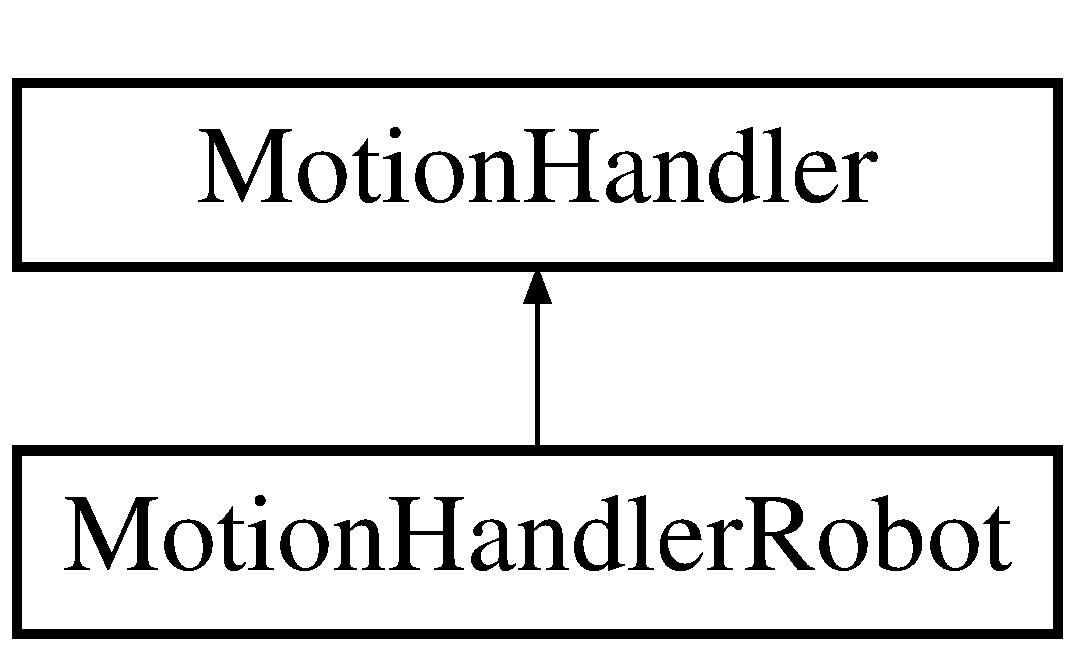
\includegraphics[height=2.000000cm]{class_motion_handler}
\end{center}
\end{figure}
\subsection*{Public Member Functions}
\begin{DoxyCompactItemize}
\item 
\mbox{\Hypertarget{class_motion_handler_a48c0070bfda6acb8a7493eb7fe1200c4}\label{class_motion_handler_a48c0070bfda6acb8a7493eb7fe1200c4}} 
\mbox{\hyperlink{class_motion_handler_a48c0070bfda6acb8a7493eb7fe1200c4}{Motion\+Handler}} (\mbox{\hyperlink{class_arena_mobile_entity}{Arena\+Mobile\+Entity}} $\ast$ent)
\begin{DoxyCompactList}\small\item\em Constructor. \end{DoxyCompactList}\item 
\mbox{\Hypertarget{class_motion_handler_a91dc98beab9d5ccce6b6c18ce32c0488}\label{class_motion_handler_a91dc98beab9d5ccce6b6c18ce32c0488}} 
{\bfseries Motion\+Handler} (const \mbox{\hyperlink{class_motion_handler}{Motion\+Handler}} \&other)=default
\item 
\mbox{\Hypertarget{class_motion_handler_ad45188f2d9794fd2b257d586a7b522e6}\label{class_motion_handler_ad45188f2d9794fd2b257d586a7b522e6}} 
\mbox{\hyperlink{class_motion_handler}{Motion\+Handler}} \& {\bfseries operator=} (const \mbox{\hyperlink{class_motion_handler}{Motion\+Handler}} \&other)=default
\item 
\mbox{\Hypertarget{class_motion_handler_a44b092d9627f25f57c50ec8886d0bc29}\label{class_motion_handler_a44b092d9627f25f57c50ec8886d0bc29}} 
virtual void \mbox{\hyperlink{class_motion_handler_a44b092d9627f25f57c50ec8886d0bc29}{Update\+Velocity}} ()
\begin{DoxyCompactList}\small\item\em Update the heading angle according to the touch sensor reading. \end{DoxyCompactList}\item 
\mbox{\Hypertarget{class_motion_handler_ada53f0d6e25d759fc3f45cc55d440177}\label{class_motion_handler_ada53f0d6e25d759fc3f45cc55d440177}} 
double \mbox{\hyperlink{class_motion_handler_ada53f0d6e25d759fc3f45cc55d440177}{get\+\_\+speed\+\_\+delta}} () const
\begin{DoxyCompactList}\small\item\em Getter for speed delta used when user requests speed increase. \end{DoxyCompactList}\item 
\mbox{\Hypertarget{class_motion_handler_a908b330346b3fe969684106bd5c7619d}\label{class_motion_handler_a908b330346b3fe969684106bd5c7619d}} 
void \mbox{\hyperlink{class_motion_handler_a908b330346b3fe969684106bd5c7619d}{set\+\_\+speed\+\_\+delta}} (double sd)
\begin{DoxyCompactList}\small\item\em Setter method for the speed delta. Set at initialization only. \end{DoxyCompactList}\item 
\mbox{\Hypertarget{class_motion_handler_aa5ec33068c516234a6521de356b08d68}\label{class_motion_handler_aa5ec33068c516234a6521de356b08d68}} 
double \mbox{\hyperlink{class_motion_handler_aa5ec33068c516234a6521de356b08d68}{get\+\_\+angle\+\_\+delta}} () const
\begin{DoxyCompactList}\small\item\em Getter for angle delta used when user requests turning. \end{DoxyCompactList}\item 
\mbox{\Hypertarget{class_motion_handler_a8c2811ddf1a0f077fec829c460009286}\label{class_motion_handler_a8c2811ddf1a0f077fec829c460009286}} 
void \mbox{\hyperlink{class_motion_handler_a8c2811ddf1a0f077fec829c460009286}{set\+\_\+angle\+\_\+delta}} (double ad)
\begin{DoxyCompactList}\small\item\em Setter method for the angle delta. Set at initialization only. \end{DoxyCompactList}\item 
\mbox{\Hypertarget{class_motion_handler_adfdbadc838050ee57945689183f34506}\label{class_motion_handler_adfdbadc838050ee57945689183f34506}} 
virtual void \mbox{\hyperlink{class_motion_handler_adfdbadc838050ee57945689183f34506}{Increase\+Speed}} ()
\begin{DoxyCompactList}\small\item\em Increase the overall speed of the entity by speed\+\_\+delta. \end{DoxyCompactList}\item 
\mbox{\Hypertarget{class_motion_handler_a527f08266130bceb6dc554cad9ad008b}\label{class_motion_handler_a527f08266130bceb6dc554cad9ad008b}} 
virtual void \mbox{\hyperlink{class_motion_handler_a527f08266130bceb6dc554cad9ad008b}{Decrease\+Speed}} ()
\begin{DoxyCompactList}\small\item\em Decrease the overall speed of the entity by speed\+\_\+delta. \end{DoxyCompactList}\item 
\mbox{\Hypertarget{class_motion_handler_a4299b69223b25b8f368b7b1059abbf60}\label{class_motion_handler_a4299b69223b25b8f368b7b1059abbf60}} 
virtual void \mbox{\hyperlink{class_motion_handler_a4299b69223b25b8f368b7b1059abbf60}{Turn\+Right}} ()
\begin{DoxyCompactList}\small\item\em Turn the entity to the right by angle\+\_\+delta (in degrees?) \end{DoxyCompactList}\item 
\mbox{\Hypertarget{class_motion_handler_a8af761f4ada79a6685e7e6dd4d23657e}\label{class_motion_handler_a8af761f4ada79a6685e7e6dd4d23657e}} 
virtual void \mbox{\hyperlink{class_motion_handler_a8af761f4ada79a6685e7e6dd4d23657e}{Turn\+Left}} ()
\begin{DoxyCompactList}\small\item\em Turn the entity to the left by angle\+\_\+delta (in degrees?) \end{DoxyCompactList}\item 
\mbox{\Hypertarget{class_motion_handler_a71e2e4cdddfb8c49eb18cf41878a08c0}\label{class_motion_handler_a71e2e4cdddfb8c49eb18cf41878a08c0}} 
double \mbox{\hyperlink{class_motion_handler_a71e2e4cdddfb8c49eb18cf41878a08c0}{get\+\_\+max\+\_\+speed}} () const
\begin{DoxyCompactList}\small\item\em Getter method for the maximum speed of entity. \end{DoxyCompactList}\item 
\mbox{\Hypertarget{class_motion_handler_a32e832d35e73e9db85c16b3ff569196e}\label{class_motion_handler_a32e832d35e73e9db85c16b3ff569196e}} 
void \mbox{\hyperlink{class_motion_handler_a32e832d35e73e9db85c16b3ff569196e}{set\+\_\+max\+\_\+speed}} (double ms)
\begin{DoxyCompactList}\small\item\em Setter method for the maximum speed. Set at initialization only. \end{DoxyCompactList}\item 
\mbox{\Hypertarget{class_motion_handler_af6ef42cdbf31ec1589e14d5dfd639d79}\label{class_motion_handler_af6ef42cdbf31ec1589e14d5dfd639d79}} 
double \mbox{\hyperlink{class_motion_handler_af6ef42cdbf31ec1589e14d5dfd639d79}{get\+\_\+max\+\_\+angle}} () const
\begin{DoxyCompactList}\small\item\em Getter method for the maximum angle. \end{DoxyCompactList}\item 
\mbox{\Hypertarget{class_motion_handler_aa73973c705626f1f95ac59391f23bcc9}\label{class_motion_handler_aa73973c705626f1f95ac59391f23bcc9}} 
void \mbox{\hyperlink{class_motion_handler_aa73973c705626f1f95ac59391f23bcc9}{set\+\_\+max\+\_\+angle}} (double ma)
\begin{DoxyCompactList}\small\item\em Setter method for the maximum angle. Set at initialization only. \end{DoxyCompactList}\item 
\mbox{\Hypertarget{class_motion_handler_abe03a52474984233d1867405925a4102}\label{class_motion_handler_abe03a52474984233d1867405925a4102}} 
\mbox{\hyperlink{struct_wheel_velocity}{Wheel\+Velocity}} \mbox{\hyperlink{class_motion_handler_abe03a52474984233d1867405925a4102}{get\+\_\+velocity}} () const
\begin{DoxyCompactList}\small\item\em Getter for \mbox{\hyperlink{struct_wheel_velocity}{Wheel\+Velocity}} struct, which has a .left and .right value. \end{DoxyCompactList}\item 
\mbox{\Hypertarget{class_motion_handler_ac4bf67ba783c1afb5a5839229de3f3f9}\label{class_motion_handler_ac4bf67ba783c1afb5a5839229de3f3f9}} 
void \mbox{\hyperlink{class_motion_handler_ac4bf67ba783c1afb5a5839229de3f3f9}{set\+\_\+velocity}} (\mbox{\hyperlink{struct_wheel_velocity}{Wheel\+Velocity}} vel)
\begin{DoxyCompactList}\small\item\em Setter for \mbox{\hyperlink{struct_wheel_velocity}{Wheel\+Velocity}} struct with struct as input param. \end{DoxyCompactList}\item 
\mbox{\Hypertarget{class_motion_handler_af31975aa667ca20835e4d5bb0216706e}\label{class_motion_handler_af31975aa667ca20835e4d5bb0216706e}} 
void \mbox{\hyperlink{class_motion_handler_af31975aa667ca20835e4d5bb0216706e}{set\+\_\+velocity}} (double vl, double vr)
\begin{DoxyCompactList}\small\item\em Setter for \mbox{\hyperlink{struct_wheel_velocity}{Wheel\+Velocity}} struct with input params of .left and .right components. \end{DoxyCompactList}\item 
\mbox{\Hypertarget{class_motion_handler_ad8472612d15be1ada7f919f45d245adc}\label{class_motion_handler_ad8472612d15be1ada7f919f45d245adc}} 
\mbox{\hyperlink{class_arena_mobile_entity}{Arena\+Mobile\+Entity}} $\ast$ {\bfseries get\+\_\+entity} ()
\end{DoxyCompactItemize}
\subsection*{Protected Attributes}
\begin{DoxyCompactItemize}
\item 
\mbox{\Hypertarget{class_motion_handler_a659fd1ec8878260a63779bf45681f5a4}\label{class_motion_handler_a659fd1ec8878260a63779bf45681f5a4}} 
\mbox{\hyperlink{class_arena_mobile_entity}{Arena\+Mobile\+Entity}} $\ast$ {\bfseries entity\+\_\+}
\end{DoxyCompactItemize}


\subsection{Detailed Description}
\mbox{\hyperlink{class_food}{Food}} class for managing the pose and wheel velocity of the entity. 

The pose.\+heading will change when the entity collides. The pose position will change at each timestep, which is determined by the motion behavior, not the handler. The pose.\+heading might change at each timestep (if wheel velocities are not equivalent), again determined by the motion behavior. 

The documentation for this class was generated from the following files\+:\begin{DoxyCompactItemize}
\item 
src/\mbox{\hyperlink{motion__handler_8h}{motion\+\_\+handler.\+h}}\item 
src/\mbox{\hyperlink{motion__handler_8cc}{motion\+\_\+handler.\+cc}}\end{DoxyCompactItemize}

\hypertarget{class_motion_handler_robot}{}\section{Motion\+Handler\+Robot Class Reference}
\label{class_motion_handler_robot}\index{Motion\+Handler\+Robot@{Motion\+Handler\+Robot}}


Class managing a \mbox{\hyperlink{class_robot}{Robot}}\textquotesingle{}s speed and heading angle foodd on collisions and user inputs.  




{\ttfamily \#include $<$motion\+\_\+handler\+\_\+robot.\+h$>$}

Inheritance diagram for Motion\+Handler\+Robot\+:\begin{figure}[H]
\begin{center}
\leavevmode
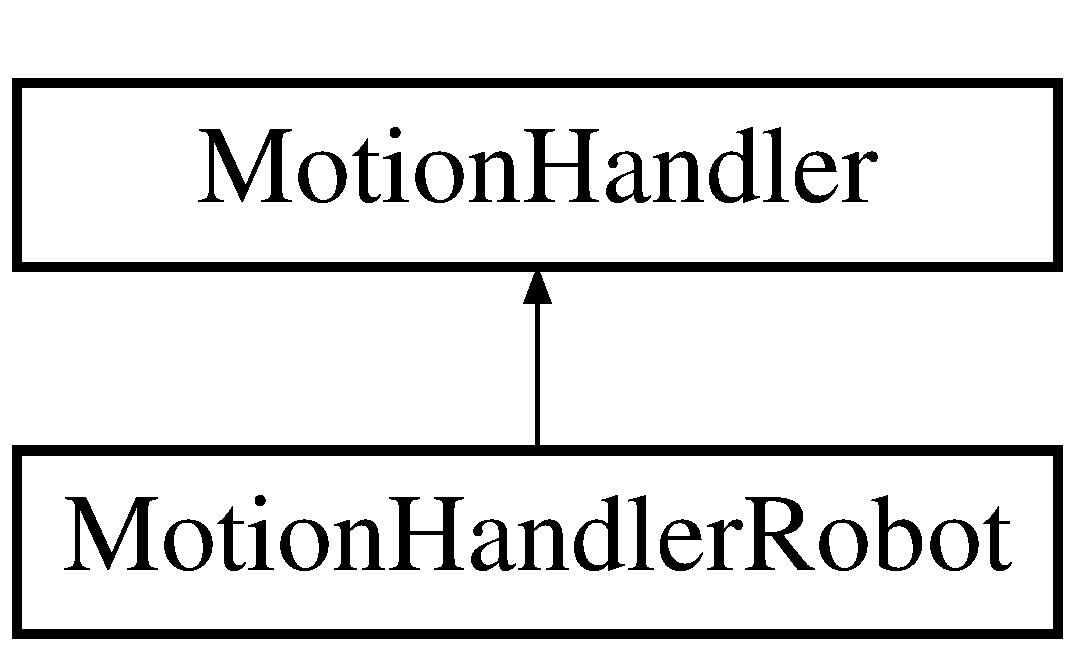
\includegraphics[height=2.000000cm]{class_motion_handler_robot}
\end{center}
\end{figure}
\subsection*{Public Member Functions}
\begin{DoxyCompactItemize}
\item 
\mbox{\Hypertarget{class_motion_handler_robot_a4b52a0b181837a8d63c39f71811d691b}\label{class_motion_handler_robot_a4b52a0b181837a8d63c39f71811d691b}} 
{\bfseries Motion\+Handler\+Robot} (\mbox{\hyperlink{class_arena_mobile_entity}{Arena\+Mobile\+Entity}} $\ast$ent)
\item 
\mbox{\Hypertarget{class_motion_handler_robot_a66445cc9057e3ef9298b5bd239df6d4e}\label{class_motion_handler_robot_a66445cc9057e3ef9298b5bd239df6d4e}} 
{\bfseries Motion\+Handler\+Robot} (const \mbox{\hyperlink{class_motion_handler_robot}{Motion\+Handler\+Robot}} \&other)=default
\item 
\mbox{\Hypertarget{class_motion_handler_robot_a48181f197ffb864f16e29721ad964e4a}\label{class_motion_handler_robot_a48181f197ffb864f16e29721ad964e4a}} 
\mbox{\hyperlink{class_motion_handler_robot}{Motion\+Handler\+Robot}} \& {\bfseries operator=} (const \mbox{\hyperlink{class_motion_handler_robot}{Motion\+Handler\+Robot}} \&other)=default
\item 
void \mbox{\hyperlink{class_motion_handler_robot_acd2cdb615d806dcf809142e84569ca9d}{Update\+Velocity}} () override
\begin{DoxyCompactList}\small\item\em Update the speed and the pose angle according to the sensor readings. \end{DoxyCompactList}\item 
\mbox{\Hypertarget{class_motion_handler_robot_a93ea16501b7b8c0bd78edb2681aa3b6d}\label{class_motion_handler_robot_a93ea16501b7b8c0bd78edb2681aa3b6d}} 
void \mbox{\hyperlink{class_motion_handler_robot_a93ea16501b7b8c0bd78edb2681aa3b6d}{Increase\+Speed}} () override
\begin{DoxyCompactList}\small\item\em Increase the overall speed of the entity by speed\+\_\+delta. \end{DoxyCompactList}\item 
\mbox{\Hypertarget{class_motion_handler_robot_a89e9b8b4e22fb021d7d67c817e66b7b2}\label{class_motion_handler_robot_a89e9b8b4e22fb021d7d67c817e66b7b2}} 
void \mbox{\hyperlink{class_motion_handler_robot_a89e9b8b4e22fb021d7d67c817e66b7b2}{Decrease\+Speed}} () override
\begin{DoxyCompactList}\small\item\em Decrease the overall speed of the entity by speed\+\_\+delta. \end{DoxyCompactList}\item 
\mbox{\Hypertarget{class_motion_handler_robot_a4b18204b7c7f7f8a3cbb7f0e8ccf088f}\label{class_motion_handler_robot_a4b18204b7c7f7f8a3cbb7f0e8ccf088f}} 
void \mbox{\hyperlink{class_motion_handler_robot_a4b18204b7c7f7f8a3cbb7f0e8ccf088f}{Turn\+Right}} () override
\begin{DoxyCompactList}\small\item\em Turn the entity to the right by angle\+\_\+delta (in degrees?) \end{DoxyCompactList}\item 
\mbox{\Hypertarget{class_motion_handler_robot_a955ca2693c4188ffb08cfde469e58252}\label{class_motion_handler_robot_a955ca2693c4188ffb08cfde469e58252}} 
void \mbox{\hyperlink{class_motion_handler_robot_a955ca2693c4188ffb08cfde469e58252}{Turn\+Left}} () override
\begin{DoxyCompactList}\small\item\em Turn the entity to the left by angle\+\_\+delta (in degrees?) \end{DoxyCompactList}\end{DoxyCompactItemize}
\subsection*{Additional Inherited Members}


\subsection{Detailed Description}
Class managing a \mbox{\hyperlink{class_robot}{Robot}}\textquotesingle{}s speed and heading angle foodd on collisions and user inputs. 

Currently, both wheels are always going at maximum speed, and cannot be controlled independently. 

\subsection{Member Function Documentation}
\mbox{\Hypertarget{class_motion_handler_robot_acd2cdb615d806dcf809142e84569ca9d}\label{class_motion_handler_robot_acd2cdb615d806dcf809142e84569ca9d}} 
\index{Motion\+Handler\+Robot@{Motion\+Handler\+Robot}!Update\+Velocity@{Update\+Velocity}}
\index{Update\+Velocity@{Update\+Velocity}!Motion\+Handler\+Robot@{Motion\+Handler\+Robot}}
\subsubsection{\texorpdfstring{Update\+Velocity()}{UpdateVelocity()}}
{\footnotesize\ttfamily void Motion\+Handler\+Robot\+::\+Update\+Velocity (\begin{DoxyParamCaption}{ }\end{DoxyParamCaption})\hspace{0.3cm}{\ttfamily [override]}, {\ttfamily [virtual]}}



Update the speed and the pose angle according to the sensor readings. 

Currently does not change speed.


\begin{DoxyParams}[1]{Parameters}
\mbox{\tt in}  & {\em pose} & The current pose. \\
\hline
\mbox{\tt in}  & {\em st} & A \mbox{\hyperlink{class_sensor_touch}{Sensor\+Touch}} to be read. \\
\hline
\end{DoxyParams}


Reimplemented from \mbox{\hyperlink{class_motion_handler_a44b092d9627f25f57c50ec8886d0bc29}{Motion\+Handler}}.



The documentation for this class was generated from the following files\+:\begin{DoxyCompactItemize}
\item 
src/\mbox{\hyperlink{motion__handler__robot_8h}{motion\+\_\+handler\+\_\+robot.\+h}}\item 
src/\mbox{\hyperlink{motion__handler__robot_8cc}{motion\+\_\+handler\+\_\+robot.\+cc}}\end{DoxyCompactItemize}

\hypertarget{struct_pose}{}\section{Pose Struct Reference}
\label{struct_pose}\index{Pose@{Pose}}


A simple representation of the position/orientation of an entity within the \mbox{\hyperlink{class_arena}{Arena}}.  




{\ttfamily \#include $<$pose.\+h$>$}

\subsection*{Public Member Functions}
\begin{DoxyCompactItemize}
\item 
\mbox{\Hypertarget{struct_pose_a8a4171c8a6b09e37fb011997da9ea2ad}\label{struct_pose_a8a4171c8a6b09e37fb011997da9ea2ad}} 
\mbox{\hyperlink{struct_pose_a8a4171c8a6b09e37fb011997da9ea2ad}{Pose}} ()
\begin{DoxyCompactList}\small\item\em Default constructor. Initialize the pose to (0,0,0) \end{DoxyCompactList}\item 
\mbox{\hyperlink{struct_pose_ac947d7046547d883f782ab2408cb80ed}{Pose}} (double in\+\_\+x, double in\+\_\+y)
\begin{DoxyCompactList}\small\item\em Constructor. \end{DoxyCompactList}\item 
\mbox{\Hypertarget{struct_pose_a6ebb8a1510c5915fa1dbec0f7ba0ad1c}\label{struct_pose_a6ebb8a1510c5915fa1dbec0f7ba0ad1c}} 
{\bfseries Pose} (double in\+\_\+x, double in\+\_\+y, double in\+\_\+theta)
\item 
\mbox{\hyperlink{struct_pose}{Pose}} \& \mbox{\hyperlink{struct_pose_aec0a9478daefa358aa2f1873cbaf0271}{operator=}} (const \mbox{\hyperlink{struct_pose}{Pose}} \&other)=default
\begin{DoxyCompactList}\small\item\em Default assignment operator. Simply copies the (x,y) values of another \mbox{\hyperlink{struct_pose}{Pose}}. \end{DoxyCompactList}\end{DoxyCompactItemize}
\subsection*{Public Attributes}
\begin{DoxyCompactItemize}
\item 
\mbox{\Hypertarget{struct_pose_a0061c7789df90f593ab95118cbef387f}\label{struct_pose_a0061c7789df90f593ab95118cbef387f}} 
double {\bfseries x} \{0\}
\item 
\mbox{\Hypertarget{struct_pose_a6280216efe0840a7a55f025ad04e3b3d}\label{struct_pose_a6280216efe0840a7a55f025ad04e3b3d}} 
double {\bfseries y} \{0\}
\item 
\mbox{\Hypertarget{struct_pose_a25709c116282114c9f512b205f3f1133}\label{struct_pose_a25709c116282114c9f512b205f3f1133}} 
double {\bfseries theta} \{0.\+0\}
\end{DoxyCompactItemize}


\subsection{Detailed Description}
A simple representation of the position/orientation of an entity within the \mbox{\hyperlink{class_arena}{Arena}}. 

N\+O\+TE\+: Origin (0,0) is at the upper left corner of the \mbox{\hyperlink{class_arena}{Arena}}. 

\subsection{Constructor \& Destructor Documentation}
\mbox{\Hypertarget{struct_pose_ac947d7046547d883f782ab2408cb80ed}\label{struct_pose_ac947d7046547d883f782ab2408cb80ed}} 
\index{Pose@{Pose}!Pose@{Pose}}
\index{Pose@{Pose}!Pose@{Pose}}
\subsubsection{\texorpdfstring{Pose()}{Pose()}}
{\footnotesize\ttfamily Pose\+::\+Pose (\begin{DoxyParamCaption}\item[{double}]{in\+\_\+x,  }\item[{double}]{in\+\_\+y }\end{DoxyParamCaption})\hspace{0.3cm}{\ttfamily [inline]}}



Constructor. 


\begin{DoxyParams}{Parameters}
{\em in\+\_\+x} & The X component of the \mbox{\hyperlink{struct_pose}{Pose}}. \\
\hline
{\em in\+\_\+y} & The Y component of the \mbox{\hyperlink{struct_pose}{Pose}}. \\
\hline
\end{DoxyParams}


\subsection{Member Function Documentation}
\mbox{\Hypertarget{struct_pose_aec0a9478daefa358aa2f1873cbaf0271}\label{struct_pose_aec0a9478daefa358aa2f1873cbaf0271}} 
\index{Pose@{Pose}!operator=@{operator=}}
\index{operator=@{operator=}!Pose@{Pose}}
\subsubsection{\texorpdfstring{operator=()}{operator=()}}
{\footnotesize\ttfamily \mbox{\hyperlink{struct_pose}{Pose}}\& Pose\+::operator= (\begin{DoxyParamCaption}\item[{const \mbox{\hyperlink{struct_pose}{Pose}} \&}]{other }\end{DoxyParamCaption})\hspace{0.3cm}{\ttfamily [default]}}



Default assignment operator. Simply copies the (x,y) values of another \mbox{\hyperlink{struct_pose}{Pose}}. 


\begin{DoxyParams}{Parameters}
{\em other} & The \mbox{\hyperlink{struct_pose}{Pose}} object to copy from.\\
\hline
\end{DoxyParams}
\begin{DoxyReturn}{Returns}
The left-\/hand-\/side \mbox{\hyperlink{struct_pose}{Pose}} object that is now identical (in value) to {\ttfamily other}. 
\end{DoxyReturn}


The documentation for this struct was generated from the following file\+:\begin{DoxyCompactItemize}
\item 
src/\mbox{\hyperlink{pose_8h}{pose.\+h}}\end{DoxyCompactItemize}

\hypertarget{struct_rgb_color}{}\section{Rgb\+Color Struct Reference}
\label{struct_rgb_color}\index{Rgb\+Color@{Rgb\+Color}}


Struct representing a rgb\+\_\+color.  




{\ttfamily \#include $<$rgb\+\_\+color.\+h$>$}

\subsection*{Public Member Functions}
\begin{DoxyCompactItemize}
\item 
\mbox{\hyperlink{struct_rgb_color_a264da0270aca412d62197e046b71b08e}{Rgb\+Color}} ()
\begin{DoxyCompactList}\small\item\em Default constructor. \end{DoxyCompactList}\item 
\mbox{\hyperlink{struct_rgb_color_a61e213533bfff019aebd27f991688222}{Rgb\+Color}} (int r\+\_\+in, int g\+\_\+in, int b\+\_\+in)
\begin{DoxyCompactList}\small\item\em Constructor for Rgb\+\_\+\+Color. \end{DoxyCompactList}\item 
\mbox{\Hypertarget{struct_rgb_color_a57fcd9161e0ee6a38e707c5002db55b8}\label{struct_rgb_color_a57fcd9161e0ee6a38e707c5002db55b8}} 
void {\bfseries Set} (Rgb\+Color\+Enum value)
\end{DoxyCompactItemize}
\subsection*{Public Attributes}
\begin{DoxyCompactItemize}
\item 
\mbox{\Hypertarget{struct_rgb_color_aa6c2fac108029c79f7cc96fb6d34717f}\label{struct_rgb_color_aa6c2fac108029c79f7cc96fb6d34717f}} 
int {\bfseries r} \{0\}
\item 
\mbox{\Hypertarget{struct_rgb_color_afbc54745bd4ed7ede168e31922143eff}\label{struct_rgb_color_afbc54745bd4ed7ede168e31922143eff}} 
int {\bfseries g} \{0\}
\item 
\mbox{\Hypertarget{struct_rgb_color_af1ba4837230cfc3b0f31454ccdb03df6}\label{struct_rgb_color_af1ba4837230cfc3b0f31454ccdb03df6}} 
int {\bfseries b} \{0\}
\end{DoxyCompactItemize}


\subsection{Detailed Description}
Struct representing a rgb\+\_\+color. 

Internally uses R\+G\+BA values to represent the rgb\+\_\+color. 

\subsection{Constructor \& Destructor Documentation}
\mbox{\Hypertarget{struct_rgb_color_a264da0270aca412d62197e046b71b08e}\label{struct_rgb_color_a264da0270aca412d62197e046b71b08e}} 
\index{Rgb\+Color@{Rgb\+Color}!Rgb\+Color@{Rgb\+Color}}
\index{Rgb\+Color@{Rgb\+Color}!Rgb\+Color@{Rgb\+Color}}
\subsubsection{\texorpdfstring{Rgb\+Color()}{RgbColor()}\hspace{0.1cm}{\footnotesize\ttfamily [1/2]}}
{\footnotesize\ttfamily Rgb\+Color\+::\+Rgb\+Color (\begin{DoxyParamCaption}{ }\end{DoxyParamCaption})\hspace{0.3cm}{\ttfamily [inline]}}



Default constructor. 

Initialize R\+GB all to 0 (k\+White). \mbox{\Hypertarget{struct_rgb_color_a61e213533bfff019aebd27f991688222}\label{struct_rgb_color_a61e213533bfff019aebd27f991688222}} 
\index{Rgb\+Color@{Rgb\+Color}!Rgb\+Color@{Rgb\+Color}}
\index{Rgb\+Color@{Rgb\+Color}!Rgb\+Color@{Rgb\+Color}}
\subsubsection{\texorpdfstring{Rgb\+Color()}{RgbColor()}\hspace{0.1cm}{\footnotesize\ttfamily [2/2]}}
{\footnotesize\ttfamily Rgb\+Color\+::\+Rgb\+Color (\begin{DoxyParamCaption}\item[{int}]{r\+\_\+in,  }\item[{int}]{g\+\_\+in,  }\item[{int}]{b\+\_\+in }\end{DoxyParamCaption})\hspace{0.3cm}{\ttfamily [inline]}}



Constructor for Rgb\+\_\+\+Color. 


\begin{DoxyParams}{Parameters}
{\em r\+\_\+in} & The R component of the rgb\+\_\+color. \\
\hline
{\em g\+\_\+in} & The G component of the rgb\+\_\+color. \\
\hline
{\em b\+\_\+in} & The B component of the rgb\+\_\+color. \\
\hline
\end{DoxyParams}


The documentation for this struct was generated from the following files\+:\begin{DoxyCompactItemize}
\item 
src/\mbox{\hyperlink{rgb__color_8h}{rgb\+\_\+color.\+h}}\item 
src/\mbox{\hyperlink{rgb__color_8cc}{rgb\+\_\+color.\+cc}}\end{DoxyCompactItemize}

\hypertarget{class_robot}{}\section{Robot Class Reference}
\label{class_robot}\index{Robot@{Robot}}


Class representing a robot within the arena.  




{\ttfamily \#include $<$robot.\+h$>$}

Inheritance diagram for Robot\+:\begin{figure}[H]
\begin{center}
\leavevmode
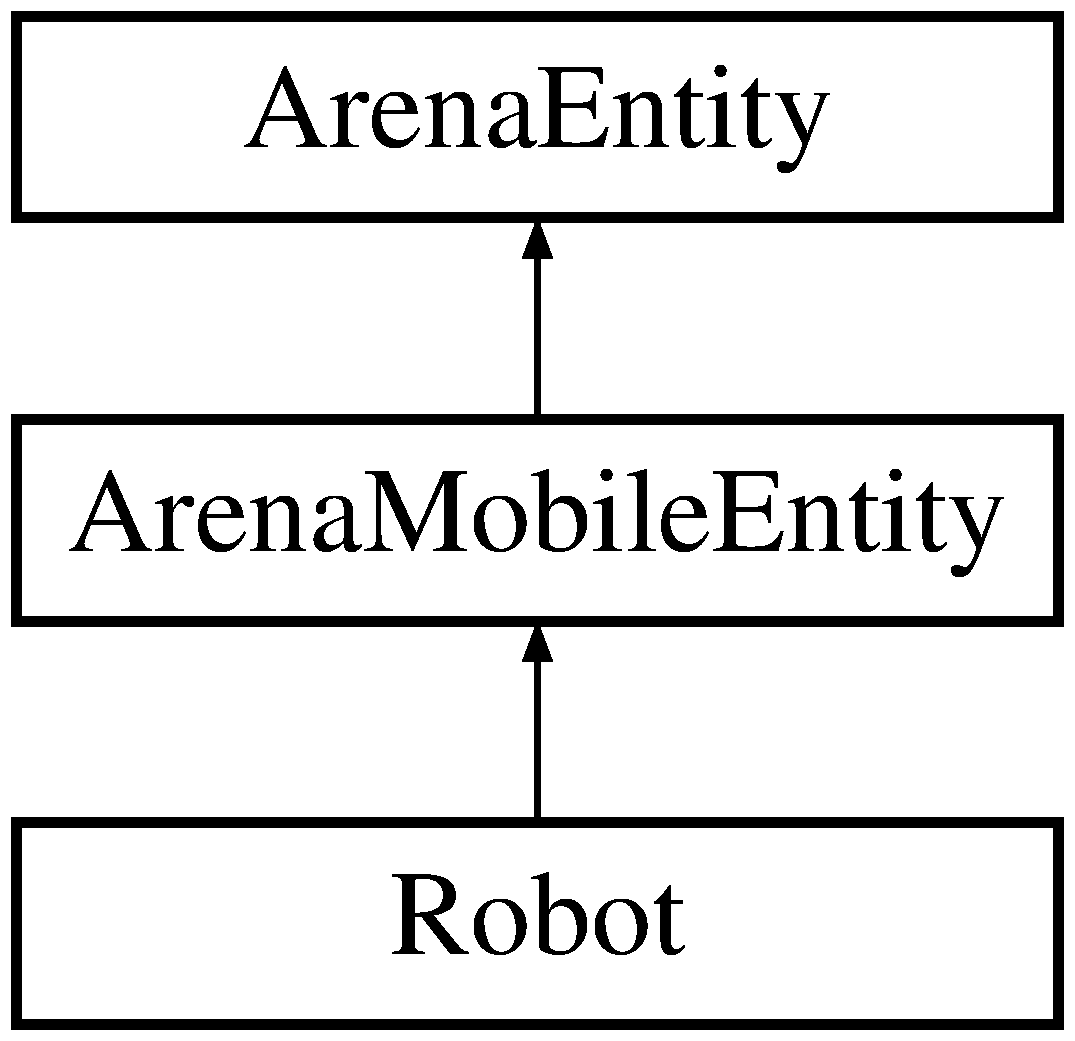
\includegraphics[height=3.000000cm]{class_robot}
\end{center}
\end{figure}
\subsection*{Public Member Functions}
\begin{DoxyCompactItemize}
\item 
\mbox{\Hypertarget{class_robot_a4fc7c70ae20623f05e06f2ecb388b6c4}\label{class_robot_a4fc7c70ae20623f05e06f2ecb388b6c4}} 
\mbox{\hyperlink{class_robot_a4fc7c70ae20623f05e06f2ecb388b6c4}{Robot}} ()
\begin{DoxyCompactList}\small\item\em Constructor using initialization values from \mbox{\hyperlink{params_8h}{params.\+h}}. \end{DoxyCompactList}\item 
\mbox{\Hypertarget{class_robot_af597fd14927d2cd5308ded62f4e54e29}\label{class_robot_af597fd14927d2cd5308ded62f4e54e29}} 
void \mbox{\hyperlink{class_robot_af597fd14927d2cd5308ded62f4e54e29}{Reset}} () override
\begin{DoxyCompactList}\small\item\em Reset the \mbox{\hyperlink{class_robot}{Robot}} to a newly constructed state (needed for reset button to work in G\+UI). \end{DoxyCompactList}\item 
void \mbox{\hyperlink{class_robot_ae790462f8782efcfd26082eedec30ed5}{Timestep\+Update}} (unsigned int dt) override
\begin{DoxyCompactList}\small\item\em Update the \mbox{\hyperlink{class_robot}{Robot}}\textquotesingle{}s position and velocity after the specified duration has passed. \end{DoxyCompactList}\item 
\mbox{\Hypertarget{class_robot_a4fc6b01fec869b559197d8e4b9686249}\label{class_robot_a4fc6b01fec869b559197d8e4b9686249}} 
void \mbox{\hyperlink{class_robot_a4fc6b01fec869b559197d8e4b9686249}{Handle\+Collision}} (Entity\+Type object\+\_\+type, \mbox{\hyperlink{class_arena_entity}{Arena\+Entity}} $\ast$object=N\+U\+LL) override
\begin{DoxyCompactList}\small\item\em Handles the collision by setting the sensor to activated. \end{DoxyCompactList}\item 
\mbox{\Hypertarget{class_robot_a3f77c13705b8f60480d21d8d936dc39e}\label{class_robot_a3f77c13705b8f60480d21d8d936dc39e}} 
std\+::string \mbox{\hyperlink{class_robot_a3f77c13705b8f60480d21d8d936dc39e}{get\+\_\+name}} () const override
\begin{DoxyCompactList}\small\item\em Get the name of the \mbox{\hyperlink{class_robot}{Robot}} for visualization and for debugging. \end{DoxyCompactList}\item 
\mbox{\Hypertarget{class_robot_ae4647cccd002ca13659017e634237ead}\label{class_robot_ae4647cccd002ca13659017e634237ead}} 
void \mbox{\hyperlink{class_robot_ae4647cccd002ca13659017e634237ead}{Increase\+Speed}} ()
\begin{DoxyCompactList}\small\item\em Command that comes from the controller, then is passed to handler. \end{DoxyCompactList}\item 
\mbox{\Hypertarget{class_robot_a94afa6f63eb22667261c07933faae481}\label{class_robot_a94afa6f63eb22667261c07933faae481}} 
void \mbox{\hyperlink{class_robot_a94afa6f63eb22667261c07933faae481}{Decrease\+Speed}} ()
\begin{DoxyCompactList}\small\item\em Command that comes from the controller, then is passed to handler. \end{DoxyCompactList}\item 
\mbox{\Hypertarget{class_robot_a12b5883779f682c66e71bc54b6539694}\label{class_robot_a12b5883779f682c66e71bc54b6539694}} 
void \mbox{\hyperlink{class_robot_a12b5883779f682c66e71bc54b6539694}{Turn\+Right}} ()
\begin{DoxyCompactList}\small\item\em Command that comes from the controller, then is passed to handler. \end{DoxyCompactList}\item 
\mbox{\Hypertarget{class_robot_ad864d21d997dbadf55f997c2f0143d41}\label{class_robot_ad864d21d997dbadf55f997c2f0143d41}} 
void \mbox{\hyperlink{class_robot_ad864d21d997dbadf55f997c2f0143d41}{Turn\+Left}} ()
\begin{DoxyCompactList}\small\item\em Command that comes from the controller, then is passed to handler. \end{DoxyCompactList}\item 
\mbox{\Hypertarget{class_robot_a66f5b5fd1597fa164a5ebaf096a5eaf1}\label{class_robot_a66f5b5fd1597fa164a5ebaf096a5eaf1}} 
int {\bfseries get\+\_\+mealtime} () const
\item 
\mbox{\Hypertarget{class_robot_a14ac367e3b1c270c31b769accdf1663c}\label{class_robot_a14ac367e3b1c270c31b769accdf1663c}} 
void {\bfseries set\+\_\+mealtime} (int l)
\item 
\mbox{\Hypertarget{class_robot_a77d37cf0058d18b7f633202e8c1bf814}\label{class_robot_a77d37cf0058d18b7f633202e8c1bf814}} 
\mbox{\hyperlink{class_motion_handler_robot}{Motion\+Handler\+Robot}} {\bfseries get\+\_\+motion\+\_\+handler} ()
\item 
\mbox{\Hypertarget{class_robot_ab45bf3c6fdafcd14cdbdb2a8e3f558b8}\label{class_robot_ab45bf3c6fdafcd14cdbdb2a8e3f558b8}} 
\mbox{\hyperlink{class_motion_behavior_differential}{Motion\+Behavior\+Differential}} {\bfseries get\+\_\+motion\+\_\+behavior} ()
\item 
\mbox{\Hypertarget{class_robot_a2573232c08bd4ec5d019d6711efa8bb3}\label{class_robot_a2573232c08bd4ec5d019d6711efa8bb3}} 
\mbox{\hyperlink{class_light_sensor}{Light\+Sensor}} \& {\bfseries get\+\_\+left} ()
\item 
\mbox{\Hypertarget{class_robot_a31c14e5da0474e3c541a3065c7326b90}\label{class_robot_a31c14e5da0474e3c541a3065c7326b90}} 
\mbox{\hyperlink{class_light_sensor}{Light\+Sensor}} \& {\bfseries get\+\_\+right} ()
\item 
\mbox{\Hypertarget{class_robot_ab68e3f017ae8d15068588958a1a09293}\label{class_robot_ab68e3f017ae8d15068588958a1a09293}} 
\mbox{\hyperlink{class_food_sensor}{Food\+Sensor}} \& {\bfseries get\+\_\+left\+Food} ()
\item 
\mbox{\Hypertarget{class_robot_a81732c5948f81a7244fa5b57b5d5174d}\label{class_robot_a81732c5948f81a7244fa5b57b5d5174d}} 
\mbox{\hyperlink{class_food_sensor}{Food\+Sensor}} \& {\bfseries get\+\_\+right\+Food} ()
\item 
\mbox{\Hypertarget{class_robot_a8464d9f4eda0441f31ced4eb452a472c}\label{class_robot_a8464d9f4eda0441f31ced4eb452a472c}} 
int {\bfseries get\+\_\+state} ()
\item 
\mbox{\Hypertarget{class_robot_a0c1e561824713bfd654873a69a7b2bae}\label{class_robot_a0c1e561824713bfd654873a69a7b2bae}} 
void {\bfseries set\+\_\+state} (int state)
\item 
\mbox{\Hypertarget{class_robot_aacdc924197b130a93046168cc31933a8}\label{class_robot_aacdc924197b130a93046168cc31933a8}} 
bool {\bfseries get\+\_\+hunger} ()
\item 
\mbox{\Hypertarget{class_robot_ac9ba3c8bdb32cf84611e82ef4fc7f5a1}\label{class_robot_ac9ba3c8bdb32cf84611e82ef4fc7f5a1}} 
void {\bfseries set\+\_\+hunger} (int state)
\item 
\mbox{\Hypertarget{class_robot_a8cacd9eb01d98a862e7e744e2855a491}\label{class_robot_a8cacd9eb01d98a862e7e744e2855a491}} 
bool {\bfseries get\+\_\+starve} ()
\item 
\mbox{\Hypertarget{class_robot_a1ba37df1aea14444965ee0ec339a7f26}\label{class_robot_a1ba37df1aea14444965ee0ec339a7f26}} 
void {\bfseries set\+\_\+starve} (int state)
\item 
\mbox{\Hypertarget{class_robot_ae4e7f627e35542a5ebc3a50e784160d2}\label{class_robot_ae4e7f627e35542a5ebc3a50e784160d2}} 
int {\bfseries get\+\_\+behave} ()
\item 
\mbox{\Hypertarget{class_robot_ab7d255b72a993d112c3da120b898ce4a}\label{class_robot_ab7d255b72a993d112c3da120b898ce4a}} 
void {\bfseries set\+\_\+behave} (int behave)
\end{DoxyCompactItemize}
\subsection*{Additional Inherited Members}


\subsection{Detailed Description}
Class representing a robot within the arena. 

Robots are composed of a motion handler, motion behavior, and touch sensor. These classes interact to maintain the pose (position and heading) of the robot. At each time step, the wheel velocities are used to calculate the next pose of the robot. The handler manages the pose and user requests. The behavior calculates the new pose foodd on wheel velocities.

Robots can be controlled through keypress, which modify wheel velocities.

The touch sensor is activated when the robot collides with an object. The heading is modified after a collision to move the robot away from the other object. 

\subsection{Member Function Documentation}
\mbox{\Hypertarget{class_robot_ae790462f8782efcfd26082eedec30ed5}\label{class_robot_ae790462f8782efcfd26082eedec30ed5}} 
\index{Robot@{Robot}!Timestep\+Update@{Timestep\+Update}}
\index{Timestep\+Update@{Timestep\+Update}!Robot@{Robot}}
\subsubsection{\texorpdfstring{Timestep\+Update()}{TimestepUpdate()}}
{\footnotesize\ttfamily void Robot\+::\+Timestep\+Update (\begin{DoxyParamCaption}\item[{unsigned int}]{dt }\end{DoxyParamCaption})\hspace{0.3cm}{\ttfamily [override]}}



Update the \mbox{\hyperlink{class_robot}{Robot}}\textquotesingle{}s position and velocity after the specified duration has passed. 


\begin{DoxyParams}{Parameters}
{\em dt} & The \# of timesteps that have elapsed since the last update. \\
\hline
\end{DoxyParams}


The documentation for this class was generated from the following files\+:\begin{DoxyCompactItemize}
\item 
src/\mbox{\hyperlink{robot_8h}{robot.\+h}}\item 
src/\mbox{\hyperlink{robot_8cc}{robot.\+cc}}\end{DoxyCompactItemize}

\hypertarget{class_sensor}{}\section{Sensor Class Reference}
\label{class_sensor}\index{Sensor@{Sensor}}


Class representing a sensor.  




{\ttfamily \#include $<$sensor.\+h$>$}

Inheritance diagram for Sensor\+:\begin{figure}[H]
\begin{center}
\leavevmode
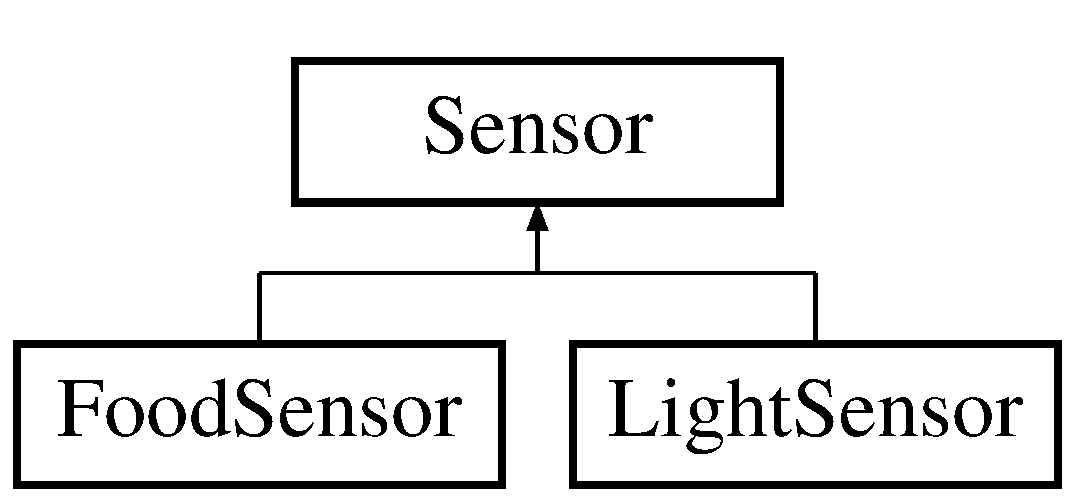
\includegraphics[height=2.000000cm]{class_sensor}
\end{center}
\end{figure}
\subsection*{Public Member Functions}
\begin{DoxyCompactItemize}
\item 
\mbox{\Hypertarget{class_sensor_a8b559df119764bb2f85d72116dacdb71}\label{class_sensor_a8b559df119764bb2f85d72116dacdb71}} 
{\bfseries Sensor} (int xpos, int ypos)
\item 
\mbox{\Hypertarget{class_sensor_a7bcda7b39b3c738116cdbbe2a45f9ed0}\label{class_sensor_a7bcda7b39b3c738116cdbbe2a45f9ed0}} 
void {\bfseries Calculate\+Reading} (int x, int y)
\item 
\mbox{\Hypertarget{class_sensor_a01eeddbc642c27e3aeb232d2a15c4a75}\label{class_sensor_a01eeddbc642c27e3aeb232d2a15c4a75}} 
void {\bfseries setconstant} (int sense)
\item 
\mbox{\Hypertarget{class_sensor_a6cde7ca5e60c12b56cb87a9859991de2}\label{class_sensor_a6cde7ca5e60c12b56cb87a9859991de2}} 
void {\bfseries Reset\+Reading} ()
\item 
\mbox{\Hypertarget{class_sensor_a33dde25c2a380263305ebef3e158f5b0}\label{class_sensor_a33dde25c2a380263305ebef3e158f5b0}} 
int {\bfseries get\+Reading} ()
\end{DoxyCompactItemize}


\subsection{Detailed Description}
Class representing a sensor. 

This is a base sensor class that takes in the the position of the entity being sensed it then calculates the reading based on the position of that entity and its own position which it holds

Sensors are fed readings and return them when prompted. 

The documentation for this class was generated from the following files\+:\begin{DoxyCompactItemize}
\item 
src/sensor.\+h\item 
src/sensor.\+cc\end{DoxyCompactItemize}

\hypertarget{class_sensor_touch}{}\section{Sensor\+Touch Class Reference}
\label{class_sensor_touch}\index{Sensor\+Touch@{Sensor\+Touch}}


Class representing a touch sensor.  




{\ttfamily \#include $<$sensor\+\_\+touch.\+h$>$}

\subsection*{Public Member Functions}
\begin{DoxyCompactItemize}
\item 
\mbox{\Hypertarget{class_sensor_touch_ab8e0dc693ec2fbc1aa5ff25ee2bfdb19}\label{class_sensor_touch_ab8e0dc693ec2fbc1aa5ff25ee2bfdb19}} 
\mbox{\hyperlink{class_sensor_touch_ab8e0dc693ec2fbc1aa5ff25ee2bfdb19}{Sensor\+Touch}} ()
\begin{DoxyCompactList}\small\item\em Constructor. \end{DoxyCompactList}\item 
const \mbox{\hyperlink{struct_pose}{Pose}} \& \mbox{\hyperlink{class_sensor_touch_a9f56fd943758125611863ce2bc0d9365}{get\+\_\+point\+\_\+of\+\_\+contact}} ()
\begin{DoxyCompactList}\small\item\em Getter method for the point of contact. \end{DoxyCompactList}\item 
void \mbox{\hyperlink{class_sensor_touch_a2ef6d89a8e763e21f82e03a3033a490f}{set\+\_\+point\+\_\+of\+\_\+contact}} (const \mbox{\hyperlink{struct_pose}{Pose}} \&p)
\begin{DoxyCompactList}\small\item\em Setter method for the point of contact. \end{DoxyCompactList}\item 
\mbox{\Hypertarget{class_sensor_touch_a0f48ab24f852395dbec807fe652d80b1}\label{class_sensor_touch_a0f48ab24f852395dbec807fe652d80b1}} 
bool \mbox{\hyperlink{class_sensor_touch_a0f48ab24f852395dbec807fe652d80b1}{get\+\_\+output}} () const
\begin{DoxyCompactList}\small\item\em Getter for output, which is true when collision occurs. \end{DoxyCompactList}\item 
void \mbox{\hyperlink{class_sensor_touch_a1980b126f7c6d0e6bdf75f1bb59fe5c2}{Handle\+Collision}} (\mbox{\hyperlink{common_8h_a2e3484535ee610c8e19e9859563abe48}{\+\_\+\+\_\+unused}} Entity\+Type object\+\_\+type, \mbox{\hyperlink{common_8h_a2e3484535ee610c8e19e9859563abe48}{\+\_\+\+\_\+unused}} \mbox{\hyperlink{class_arena_entity}{Arena\+Entity}} $\ast$object)
\begin{DoxyCompactList}\small\item\em Modify heading to presumably move away from collision. \end{DoxyCompactList}\item 
\mbox{\Hypertarget{class_sensor_touch_ad0054916c97844a51052e5dee63f68b9}\label{class_sensor_touch_ad0054916c97844a51052e5dee63f68b9}} 
void \mbox{\hyperlink{class_sensor_touch_ad0054916c97844a51052e5dee63f68b9}{Reset}} ()
\begin{DoxyCompactList}\small\item\em Reset the sensor. \end{DoxyCompactList}\end{DoxyCompactItemize}


\subsection{Detailed Description}
Class representing a touch sensor. 

Touch or \char`\"{}bump\char`\"{} sensors are \char`\"{}active\char`\"{} when pressed. For our purposes, imagine a series of bump sensors around the perimeter of an entity. A collision will activate the sensor at a particular point of contact, which translates to an angle of contact.

\mbox{\hyperlink{class_sensor_touch}{Sensor\+Touch}} can be observed for collision events. 

\subsection{Member Function Documentation}
\mbox{\Hypertarget{class_sensor_touch_a9f56fd943758125611863ce2bc0d9365}\label{class_sensor_touch_a9f56fd943758125611863ce2bc0d9365}} 
\index{Sensor\+Touch@{Sensor\+Touch}!get\+\_\+point\+\_\+of\+\_\+contact@{get\+\_\+point\+\_\+of\+\_\+contact}}
\index{get\+\_\+point\+\_\+of\+\_\+contact@{get\+\_\+point\+\_\+of\+\_\+contact}!Sensor\+Touch@{Sensor\+Touch}}
\subsubsection{\texorpdfstring{get\+\_\+point\+\_\+of\+\_\+contact()}{get\_point\_of\_contact()}}
{\footnotesize\ttfamily const \mbox{\hyperlink{struct_pose}{Pose}}\& Sensor\+Touch\+::get\+\_\+point\+\_\+of\+\_\+contact (\begin{DoxyParamCaption}{ }\end{DoxyParamCaption})\hspace{0.3cm}{\ttfamily [inline]}}



Getter method for the point of contact. 

Should only be called when the sensor is activated.

\begin{DoxyReturn}{Returns}
The latest point of contact. 
\end{DoxyReturn}
\mbox{\Hypertarget{class_sensor_touch_a1980b126f7c6d0e6bdf75f1bb59fe5c2}\label{class_sensor_touch_a1980b126f7c6d0e6bdf75f1bb59fe5c2}} 
\index{Sensor\+Touch@{Sensor\+Touch}!Handle\+Collision@{Handle\+Collision}}
\index{Handle\+Collision@{Handle\+Collision}!Sensor\+Touch@{Sensor\+Touch}}
\subsubsection{\texorpdfstring{Handle\+Collision()}{HandleCollision()}}
{\footnotesize\ttfamily void Sensor\+Touch\+::\+Handle\+Collision (\begin{DoxyParamCaption}\item[{\mbox{\hyperlink{common_8h_a2e3484535ee610c8e19e9859563abe48}{\+\_\+\+\_\+unused}} Entity\+Type}]{object\+\_\+type,  }\item[{\mbox{\hyperlink{common_8h_a2e3484535ee610c8e19e9859563abe48}{\+\_\+\+\_\+unused}} \mbox{\hyperlink{class_arena_entity}{Arena\+Entity}} $\ast$}]{object }\end{DoxyParamCaption})}



Modify heading to presumably move away from collision. 

Currently, no information is used to determine point of contact. The heading should really only change when it collides with something in front of it (as opposed to something running into the entity from behind.) The \mbox{\hyperlink{class_arena_entity}{Arena\+Entity}} can be used to determine the point of contact. \mbox{\Hypertarget{class_sensor_touch_a2ef6d89a8e763e21f82e03a3033a490f}\label{class_sensor_touch_a2ef6d89a8e763e21f82e03a3033a490f}} 
\index{Sensor\+Touch@{Sensor\+Touch}!set\+\_\+point\+\_\+of\+\_\+contact@{set\+\_\+point\+\_\+of\+\_\+contact}}
\index{set\+\_\+point\+\_\+of\+\_\+contact@{set\+\_\+point\+\_\+of\+\_\+contact}!Sensor\+Touch@{Sensor\+Touch}}
\subsubsection{\texorpdfstring{set\+\_\+point\+\_\+of\+\_\+contact()}{set\_point\_of\_contact()}}
{\footnotesize\ttfamily void Sensor\+Touch\+::set\+\_\+point\+\_\+of\+\_\+contact (\begin{DoxyParamCaption}\item[{const \mbox{\hyperlink{struct_pose}{Pose}} \&}]{p }\end{DoxyParamCaption})\hspace{0.3cm}{\ttfamily [inline]}}



Setter method for the point of contact. 


\begin{DoxyParams}{Parameters}
{\em p} & The new point of contact. \\
\hline
\end{DoxyParams}


The documentation for this class was generated from the following files\+:\begin{DoxyCompactItemize}
\item 
src/\mbox{\hyperlink{sensor__touch_8h}{sensor\+\_\+touch.\+h}}\item 
src/\mbox{\hyperlink{sensor__touch_8cc}{sensor\+\_\+touch.\+cc}}\end{DoxyCompactItemize}

\hypertarget{struct_wheel_velocity}{}\section{Wheel\+Velocity Struct Reference}
\label{struct_wheel_velocity}\index{Wheel\+Velocity@{Wheel\+Velocity}}


A simple representation of the position/orientation of an entity within the \mbox{\hyperlink{class_arena}{Arena}}.  




{\ttfamily \#include $<$wheel\+\_\+velocity.\+h$>$}

\subsection*{Public Member Functions}
\begin{DoxyCompactItemize}
\item 
\mbox{\Hypertarget{struct_wheel_velocity_a20d96cc07cac3a0ebaea27e852f262a7}\label{struct_wheel_velocity_a20d96cc07cac3a0ebaea27e852f262a7}} 
\mbox{\hyperlink{struct_wheel_velocity_a20d96cc07cac3a0ebaea27e852f262a7}{Wheel\+Velocity}} ()
\begin{DoxyCompactList}\small\item\em Default constructor. Initialize the pose to (0,0,0) \end{DoxyCompactList}\item 
\mbox{\hyperlink{struct_wheel_velocity_a08a753191ddcffb83592d60e4e46be65}{Wheel\+Velocity}} (double l, double r)
\begin{DoxyCompactList}\small\item\em Constructor. \end{DoxyCompactList}\item 
\mbox{\hyperlink{struct_wheel_velocity}{Wheel\+Velocity}} \& \mbox{\hyperlink{struct_wheel_velocity_a43eee436deaaa5fb6e0d747c2cc4d266}{operator=}} (const \mbox{\hyperlink{struct_wheel_velocity}{Wheel\+Velocity}} \&other)=default
\begin{DoxyCompactList}\small\item\em Default assignment operator. Simply copies the (x,y) values of another \mbox{\hyperlink{struct_pose}{Pose}}. \end{DoxyCompactList}\end{DoxyCompactItemize}
\subsection*{Public Attributes}
\begin{DoxyCompactItemize}
\item 
\mbox{\Hypertarget{struct_wheel_velocity_a16cfad265d944e9734d1dfa198c98438}\label{struct_wheel_velocity_a16cfad265d944e9734d1dfa198c98438}} 
double {\bfseries left}
\item 
\mbox{\Hypertarget{struct_wheel_velocity_a7aa2910779ef5ed0b2975d8675918a6a}\label{struct_wheel_velocity_a7aa2910779ef5ed0b2975d8675918a6a}} 
double {\bfseries right}
\end{DoxyCompactItemize}


\subsection{Detailed Description}
A simple representation of the position/orientation of an entity within the \mbox{\hyperlink{class_arena}{Arena}}. 

N\+O\+TE\+: Origin (0,0) is at the upper left corner of the \mbox{\hyperlink{class_arena}{Arena}}. 

\subsection{Constructor \& Destructor Documentation}
\mbox{\Hypertarget{struct_wheel_velocity_a08a753191ddcffb83592d60e4e46be65}\label{struct_wheel_velocity_a08a753191ddcffb83592d60e4e46be65}} 
\index{Wheel\+Velocity@{Wheel\+Velocity}!Wheel\+Velocity@{Wheel\+Velocity}}
\index{Wheel\+Velocity@{Wheel\+Velocity}!Wheel\+Velocity@{Wheel\+Velocity}}
\subsubsection{\texorpdfstring{Wheel\+Velocity()}{WheelVelocity()}}
{\footnotesize\ttfamily Wheel\+Velocity\+::\+Wheel\+Velocity (\begin{DoxyParamCaption}\item[{double}]{l,  }\item[{double}]{r }\end{DoxyParamCaption})\hspace{0.3cm}{\ttfamily [inline]}}



Constructor. 


\begin{DoxyParams}{Parameters}
{\em in\+\_\+x} & The X component of the \mbox{\hyperlink{struct_pose}{Pose}}. \\
\hline
{\em in\+\_\+y} & The Y component of the \mbox{\hyperlink{struct_pose}{Pose}}. \\
\hline
\end{DoxyParams}


\subsection{Member Function Documentation}
\mbox{\Hypertarget{struct_wheel_velocity_a43eee436deaaa5fb6e0d747c2cc4d266}\label{struct_wheel_velocity_a43eee436deaaa5fb6e0d747c2cc4d266}} 
\index{Wheel\+Velocity@{Wheel\+Velocity}!operator=@{operator=}}
\index{operator=@{operator=}!Wheel\+Velocity@{Wheel\+Velocity}}
\subsubsection{\texorpdfstring{operator=()}{operator=()}}
{\footnotesize\ttfamily \mbox{\hyperlink{struct_wheel_velocity}{Wheel\+Velocity}}\& Wheel\+Velocity\+::operator= (\begin{DoxyParamCaption}\item[{const \mbox{\hyperlink{struct_wheel_velocity}{Wheel\+Velocity}} \&}]{other }\end{DoxyParamCaption})\hspace{0.3cm}{\ttfamily [default]}}



Default assignment operator. Simply copies the (x,y) values of another \mbox{\hyperlink{struct_pose}{Pose}}. 


\begin{DoxyParams}{Parameters}
{\em other} & The \mbox{\hyperlink{struct_pose}{Pose}} object to copy from.\\
\hline
\end{DoxyParams}
\begin{DoxyReturn}{Returns}
The left-\/hand-\/side \mbox{\hyperlink{struct_pose}{Pose}} object that is now identical (in value) to {\ttfamily other}. 
\end{DoxyReturn}


The documentation for this struct was generated from the following file\+:\begin{DoxyCompactItemize}
\item 
src/\mbox{\hyperlink{wheel__velocity_8h}{wheel\+\_\+velocity.\+h}}\end{DoxyCompactItemize}

\chapter{File Documentation}
\hypertarget{arena_8cc}{}\section{src/arena.cc File Reference}
\label{arena_8cc}\index{src/arena.\+cc@{src/arena.\+cc}}
{\ttfamily \#include $<$algorithm$>$}\newline
{\ttfamily \#include $<$iostream$>$}\newline
{\ttfamily \#include \char`\"{}src/arena.\+h\char`\"{}}\newline
{\ttfamily \#include \char`\"{}src/arena\+\_\+params.\+h\char`\"{}}\newline
\subsection*{Functions}
\begin{DoxyCompactItemize}
\item 
\mbox{\Hypertarget{arena_8cc_a5eaf22d0e7e2a0f12c6a660a6b011297}\label{arena_8cc_a5eaf22d0e7e2a0f12c6a660a6b011297}} 
{\bfseries N\+A\+M\+E\+S\+P\+A\+C\+E\+\_\+\+B\+E\+G\+IN} (csci3081)
\item 
\mbox{\Hypertarget{arena_8cc_a0bc8eb973c3aef52acd7429898ace1cd}\label{arena_8cc_a0bc8eb973c3aef52acd7429898ace1cd}} 
{\bfseries N\+A\+M\+E\+S\+P\+A\+C\+E\+\_\+\+E\+ND} (csci3081)
\end{DoxyCompactItemize}


\subsection{Detailed Description}
\begin{DoxyCopyright}{Copyright}
2017 3081 Staff, All rights reserved. 
\end{DoxyCopyright}

\hypertarget{arena_8h}{}\section{src/arena.h File Reference}
\label{arena_8h}\index{src/arena.\+h@{src/arena.\+h}}
{\ttfamily \#include $<$cmath$>$}\newline
{\ttfamily \#include $<$iostream$>$}\newline
{\ttfamily \#include $<$vector$>$}\newline
{\ttfamily \#include \char`\"{}src/common.\+h\char`\"{}}\newline
{\ttfamily \#include \char`\"{}src/food.\+h\char`\"{}}\newline
{\ttfamily \#include \char`\"{}src/entity\+\_\+factory.\+h\char`\"{}}\newline
{\ttfamily \#include \char`\"{}src/robot.\+h\char`\"{}}\newline
{\ttfamily \#include \char`\"{}src/communication.\+h\char`\"{}}\newline
\subsection*{Classes}
\begin{DoxyCompactItemize}
\item 
class \mbox{\hyperlink{class_arena}{Arena}}
\begin{DoxyCompactList}\small\item\em The main class for the simulation of a 2D world with many entities running around. \end{DoxyCompactList}\end{DoxyCompactItemize}
\subsection*{Functions}
\begin{DoxyCompactItemize}
\item 
\mbox{\Hypertarget{arena_8h_a5eaf22d0e7e2a0f12c6a660a6b011297}\label{arena_8h_a5eaf22d0e7e2a0f12c6a660a6b011297}} 
{\bfseries N\+A\+M\+E\+S\+P\+A\+C\+E\+\_\+\+B\+E\+G\+IN} (csci3081)
\item 
\mbox{\Hypertarget{arena_8h_a0bc8eb973c3aef52acd7429898ace1cd}\label{arena_8h_a0bc8eb973c3aef52acd7429898ace1cd}} 
{\bfseries N\+A\+M\+E\+S\+P\+A\+C\+E\+\_\+\+E\+ND} (csci3081)
\end{DoxyCompactItemize}


\subsection{Detailed Description}
\begin{DoxyCopyright}{Copyright}
2017 3081 Staff, All rights reserved. 
\end{DoxyCopyright}

\hypertarget{arena__entity_8h}{}\section{src/arena\+\_\+entity.h File Reference}
\label{arena__entity_8h}\index{src/arena\+\_\+entity.\+h@{src/arena\+\_\+entity.\+h}}
{\ttfamily \#include $<$string$>$}\newline
{\ttfamily \#include \char`\"{}src/common.\+h\char`\"{}}\newline
{\ttfamily \#include \char`\"{}src/entity\+\_\+type.\+h\char`\"{}}\newline
{\ttfamily \#include \char`\"{}src/params.\+h\char`\"{}}\newline
{\ttfamily \#include \char`\"{}src/pose.\+h\char`\"{}}\newline
{\ttfamily \#include \char`\"{}src/rgb\+\_\+color.\+h\char`\"{}}\newline
\subsection*{Classes}
\begin{DoxyCompactItemize}
\item 
class \mbox{\hyperlink{class_arena_entity}{Arena\+Entity}}
\begin{DoxyCompactList}\small\item\em A food class from which all \mbox{\hyperlink{class_arena}{Arena}} entities inherit. \end{DoxyCompactList}\end{DoxyCompactItemize}
\subsection*{Functions}
\begin{DoxyCompactItemize}
\item 
\mbox{\Hypertarget{arena__entity_8h_a5eaf22d0e7e2a0f12c6a660a6b011297}\label{arena__entity_8h_a5eaf22d0e7e2a0f12c6a660a6b011297}} 
{\bfseries N\+A\+M\+E\+S\+P\+A\+C\+E\+\_\+\+B\+E\+G\+IN} (csci3081)
\item 
\mbox{\Hypertarget{arena__entity_8h_a0bc8eb973c3aef52acd7429898ace1cd}\label{arena__entity_8h_a0bc8eb973c3aef52acd7429898ace1cd}} 
{\bfseries N\+A\+M\+E\+S\+P\+A\+C\+E\+\_\+\+E\+ND} (csci3081)
\end{DoxyCompactItemize}


\subsection{Detailed Description}
\begin{DoxyCopyright}{Copyright}
2017 3081 Staff, All rights reserved. 
\end{DoxyCopyright}

\hypertarget{arena__immobile__entity_8h}{}\section{src/arena\+\_\+immobile\+\_\+entity.h File Reference}
\label{arena__immobile__entity_8h}\index{src/arena\+\_\+immobile\+\_\+entity.\+h@{src/arena\+\_\+immobile\+\_\+entity.\+h}}
{\ttfamily \#include \char`\"{}src/arena\+\_\+entity.\+h\char`\"{}}\newline
{\ttfamily \#include \char`\"{}src/common.\+h\char`\"{}}\newline
\subsection*{Classes}
\begin{DoxyCompactItemize}
\item 
class \mbox{\hyperlink{class_arena_immobile_entity}{Arena\+Immobile\+Entity}}
\begin{DoxyCompactList}\small\item\em An immobile entity in the \mbox{\hyperlink{class_arena}{Arena}}. \end{DoxyCompactList}\end{DoxyCompactItemize}
\subsection*{Functions}
\begin{DoxyCompactItemize}
\item 
\mbox{\Hypertarget{arena__immobile__entity_8h_a5eaf22d0e7e2a0f12c6a660a6b011297}\label{arena__immobile__entity_8h_a5eaf22d0e7e2a0f12c6a660a6b011297}} 
{\bfseries N\+A\+M\+E\+S\+P\+A\+C\+E\+\_\+\+B\+E\+G\+IN} (csci3081)
\item 
\mbox{\Hypertarget{arena__immobile__entity_8h_a0bc8eb973c3aef52acd7429898ace1cd}\label{arena__immobile__entity_8h_a0bc8eb973c3aef52acd7429898ace1cd}} 
{\bfseries N\+A\+M\+E\+S\+P\+A\+C\+E\+\_\+\+E\+ND} (csci3081)
\end{DoxyCompactItemize}


\subsection{Detailed Description}
\begin{DoxyCopyright}{Copyright}
2017 3081 Staff, All rights reserved. 
\end{DoxyCopyright}

\hypertarget{arena__mobile__entity_8h}{}\section{src/arena\+\_\+mobile\+\_\+entity.h File Reference}
\label{arena__mobile__entity_8h}\index{src/arena\+\_\+mobile\+\_\+entity.\+h@{src/arena\+\_\+mobile\+\_\+entity.\+h}}
{\ttfamily \#include $<$algorithm$>$}\newline
{\ttfamily \#include \char`\"{}src/arena\+\_\+entity.\+h\char`\"{}}\newline
{\ttfamily \#include \char`\"{}src/common.\+h\char`\"{}}\newline
{\ttfamily \#include \char`\"{}src/sensor\+\_\+touch.\+h\char`\"{}}\newline
\subsection*{Classes}
\begin{DoxyCompactItemize}
\item 
class \mbox{\hyperlink{class_arena_mobile_entity}{Arena\+Mobile\+Entity}}
\begin{DoxyCompactList}\small\item\em A mobile entity in the \mbox{\hyperlink{class_arena}{Arena}}, capable of updating its own position and/or velocity when asked by the simulation. \end{DoxyCompactList}\end{DoxyCompactItemize}
\subsection*{Functions}
\begin{DoxyCompactItemize}
\item 
\mbox{\Hypertarget{arena__mobile__entity_8h_a5eaf22d0e7e2a0f12c6a660a6b011297}\label{arena__mobile__entity_8h_a5eaf22d0e7e2a0f12c6a660a6b011297}} 
{\bfseries N\+A\+M\+E\+S\+P\+A\+C\+E\+\_\+\+B\+E\+G\+IN} (csci3081)
\item 
\mbox{\Hypertarget{arena__mobile__entity_8h_a0bc8eb973c3aef52acd7429898ace1cd}\label{arena__mobile__entity_8h_a0bc8eb973c3aef52acd7429898ace1cd}} 
{\bfseries N\+A\+M\+E\+S\+P\+A\+C\+E\+\_\+\+E\+ND} (csci3081)
\end{DoxyCompactItemize}


\subsection{Detailed Description}
\begin{DoxyCopyright}{Copyright}
2017 3081 Staff, All rights reserved. 
\end{DoxyCopyright}

\hypertarget{arena__params_8h}{}\section{src/arena\+\_\+params.h File Reference}
\label{arena__params_8h}\index{src/arena\+\_\+params.\+h@{src/arena\+\_\+params.\+h}}
{\ttfamily \#include \char`\"{}src/common.\+h\char`\"{}}\newline
{\ttfamily \#include \char`\"{}src/light.\+h\char`\"{}}\newline
{\ttfamily \#include \char`\"{}src/params.\+h\char`\"{}}\newline
\subsection*{Classes}
\begin{DoxyCompactItemize}
\item 
struct \mbox{\hyperlink{structarena__params}{arena\+\_\+params}}
\begin{DoxyCompactList}\small\item\em Struct holding parameters for initializing the \mbox{\hyperlink{class_arena}{Arena}}. \end{DoxyCompactList}\end{DoxyCompactItemize}
\subsection*{Functions}
\begin{DoxyCompactItemize}
\item 
\mbox{\Hypertarget{arena__params_8h_a5eaf22d0e7e2a0f12c6a660a6b011297}\label{arena__params_8h_a5eaf22d0e7e2a0f12c6a660a6b011297}} 
{\bfseries N\+A\+M\+E\+S\+P\+A\+C\+E\+\_\+\+B\+E\+G\+IN} (csci3081)
\item 
\mbox{\Hypertarget{arena__params_8h_a0bc8eb973c3aef52acd7429898ace1cd}\label{arena__params_8h_a0bc8eb973c3aef52acd7429898ace1cd}} 
{\bfseries N\+A\+M\+E\+S\+P\+A\+C\+E\+\_\+\+E\+ND} (csci3081)
\end{DoxyCompactItemize}


\subsection{Detailed Description}
\begin{DoxyCopyright}{Copyright}
2017 3081 Staff, All rights reserved. 
\end{DoxyCopyright}

\hypertarget{common_8h}{}\section{src/common.h File Reference}
\label{common_8h}\index{src/common.\+h@{src/common.\+h}}
{\ttfamily \#include $<$random$>$}\newline
\subsection*{Macros}
\begin{DoxyCompactItemize}
\item 
\mbox{\Hypertarget{common_8h_a577cd817cb71b655998cad4387cdaeba}\label{common_8h_a577cd817cb71b655998cad4387cdaeba}} 
\#define {\bfseries N\+A\+M\+E\+S\+P\+A\+C\+E\+\_\+\+B\+E\+G\+IN}(name)~namespace name \{
\item 
\mbox{\Hypertarget{common_8h_a12bb24ea980ca8fb1f46b1992bc9c83a}\label{common_8h_a12bb24ea980ca8fb1f46b1992bc9c83a}} 
\#define {\bfseries N\+A\+M\+E\+S\+P\+A\+C\+E\+\_\+\+E\+ND}(name)~\}
\item 
\#define \mbox{\hyperlink{common_8h_a2e3484535ee610c8e19e9859563abe48}{\+\_\+\+\_\+unused}}~\+\_\+\+\_\+attribute\+\_\+\+\_\+((unused))
\end{DoxyCompactItemize}
\subsection*{Functions}
\begin{DoxyCompactItemize}
\item 
{\footnotesize template$<$typename T $>$ }\\T \mbox{\hyperlink{common_8h_ac14593f15572ef118d7bc7381b372b94}{random\+\_\+num}} (T min, T max)
\begin{DoxyCompactList}\small\item\em A template method for random number generation. \end{DoxyCompactList}\end{DoxyCompactItemize}


\subsection{Detailed Description}
\begin{DoxyCopyright}{Copyright}
2017 3081 Staff, All rights reserved. 
\end{DoxyCopyright}


\subsection{Macro Definition Documentation}
\mbox{\Hypertarget{common_8h_a2e3484535ee610c8e19e9859563abe48}\label{common_8h_a2e3484535ee610c8e19e9859563abe48}} 
\index{common.\+h@{common.\+h}!\+\_\+\+\_\+unused@{\+\_\+\+\_\+unused}}
\index{\+\_\+\+\_\+unused@{\+\_\+\+\_\+unused}!common.\+h@{common.\+h}}
\subsubsection{\texorpdfstring{\+\_\+\+\_\+unused}{\_\_unused}}
{\footnotesize\ttfamily \#define \+\_\+\+\_\+unused~\+\_\+\+\_\+attribute\+\_\+\+\_\+((unused))}

This should be placed in front of any variable defined but not used to satisfy the compiler -\/ otherwise a warning is given. 

\subsection{Function Documentation}
\mbox{\Hypertarget{common_8h_ac14593f15572ef118d7bc7381b372b94}\label{common_8h_ac14593f15572ef118d7bc7381b372b94}} 
\index{common.\+h@{common.\+h}!random\+\_\+num@{random\+\_\+num}}
\index{random\+\_\+num@{random\+\_\+num}!common.\+h@{common.\+h}}
\subsubsection{\texorpdfstring{random\+\_\+num()}{random\_num()}}
{\footnotesize\ttfamily template$<$typename T $>$ \\
T random\+\_\+num (\begin{DoxyParamCaption}\item[{T}]{min,  }\item[{T}]{max }\end{DoxyParamCaption})}



A template method for random number generation. 


\begin{DoxyTemplParams}{Template Parameters}
{\em T} & The type of the input/return values. Can be any primitive numeric type (e.\+g. {\ttfamily int}). \\
\hline
\end{DoxyTemplParams}

\begin{DoxyParams}{Parameters}
{\em min} & The (inclusive) minimum of the generated value. \\
\hline
{\em max} & The (exclusive) maximum of the generated value.\\
\hline
\end{DoxyParams}
\begin{DoxyReturn}{Returns}
A pseudo-\/randomly generated number in the range of \mbox{[}min, max).
\end{DoxyReturn}
Reference\+: \href{https://stackoverflow.com/a/19728404}{\tt https\+://stackoverflow.\+com/a/19728404} 
\hypertarget{communication_8h}{}\section{src/communication.h File Reference}
\label{communication_8h}\index{src/communication.\+h@{src/communication.\+h}}
{\ttfamily \#include \char`\"{}src/common.\+h\char`\"{}}\newline
\subsection*{Enumerations}
\begin{DoxyCompactItemize}
\item 
\mbox{\Hypertarget{communication_8h_a836c27e2d64d0efa4a526150bdf6f3e5}\label{communication_8h_a836c27e2d64d0efa4a526150bdf6f3e5}} 
enum {\bfseries Communication} \{ \newline
{\bfseries k\+Key\+Up}, 
{\bfseries k\+Key\+Down}, 
{\bfseries k\+Key\+Right}, 
{\bfseries k\+Key\+Left}, 
\newline
{\bfseries k\+Play}, 
{\bfseries k\+Pause}, 
{\bfseries k\+New\+Game}, 
{\bfseries k\+Increase\+Speed}, 
\newline
{\bfseries k\+Decrease\+Speed}, 
{\bfseries k\+Turn\+Right}, 
{\bfseries k\+Turn\+Left}, 
{\bfseries k\+Reset}, 
\newline
{\bfseries k\+Won}, 
{\bfseries k\+Lost}, 
{\bfseries k\+None}, 
{\bfseries k\+S\+Food}, 
\newline
{\bfseries k\+S\+No\+Food}
 \}
\end{DoxyCompactItemize}
\subsection*{Functions}
\begin{DoxyCompactItemize}
\item 
\mbox{\Hypertarget{communication_8h_a5eaf22d0e7e2a0f12c6a660a6b011297}\label{communication_8h_a5eaf22d0e7e2a0f12c6a660a6b011297}} 
{\bfseries N\+A\+M\+E\+S\+P\+A\+C\+E\+\_\+\+B\+E\+G\+IN} (csci3081)
\item 
\mbox{\Hypertarget{communication_8h_a0bc8eb973c3aef52acd7429898ace1cd}\label{communication_8h_a0bc8eb973c3aef52acd7429898ace1cd}} 
{\bfseries N\+A\+M\+E\+S\+P\+A\+C\+E\+\_\+\+E\+ND} (csci3081)
\end{DoxyCompactItemize}


\subsection{Detailed Description}
\begin{DoxyCopyright}{Copyright}
2017 3081 Staff, All rights reserved. 
\end{DoxyCopyright}

\hypertarget{controller_8cc}{}\section{src/controller.cc File Reference}
\label{controller_8cc}\index{src/controller.\+cc@{src/controller.\+cc}}
{\ttfamily \#include $<$nanogui/nanogui.\+h$>$}\newline
{\ttfamily \#include $<$string$>$}\newline
{\ttfamily \#include \char`\"{}src/arena\+\_\+params.\+h\char`\"{}}\newline
{\ttfamily \#include \char`\"{}src/common.\+h\char`\"{}}\newline
{\ttfamily \#include \char`\"{}src/controller.\+h\char`\"{}}\newline
\subsection*{Functions}
\begin{DoxyCompactItemize}
\item 
\mbox{\Hypertarget{controller_8cc_a5eaf22d0e7e2a0f12c6a660a6b011297}\label{controller_8cc_a5eaf22d0e7e2a0f12c6a660a6b011297}} 
{\bfseries N\+A\+M\+E\+S\+P\+A\+C\+E\+\_\+\+B\+E\+G\+IN} (csci3081)
\item 
\mbox{\Hypertarget{controller_8cc_a0bc8eb973c3aef52acd7429898ace1cd}\label{controller_8cc_a0bc8eb973c3aef52acd7429898ace1cd}} 
{\bfseries N\+A\+M\+E\+S\+P\+A\+C\+E\+\_\+\+E\+ND} (csci3081)
\end{DoxyCompactItemize}


\subsection{Detailed Description}
\begin{DoxyCopyright}{Copyright}
2017 3081 Staff, All rights reserved. 
\end{DoxyCopyright}

\hypertarget{controller_8h}{}\section{src/controller.h File Reference}
\label{controller_8h}\index{src/controller.\+h@{src/controller.\+h}}
{\ttfamily \#include $<$nanogui/nanogui.\+h$>$}\newline
{\ttfamily \#include $<$string$>$}\newline
{\ttfamily \#include \char`\"{}src/arena.\+h\char`\"{}}\newline
{\ttfamily \#include \char`\"{}src/common.\+h\char`\"{}}\newline
{\ttfamily \#include \char`\"{}src/communication.\+h\char`\"{}}\newline
{\ttfamily \#include \char`\"{}src/graphics\+\_\+arena\+\_\+viewer.\+h\char`\"{}}\newline
\subsection*{Classes}
\begin{DoxyCompactItemize}
\item 
class \mbox{\hyperlink{class_controller}{Controller}}
\begin{DoxyCompactList}\small\item\em \mbox{\hyperlink{class_controller}{Controller}} that mediates \mbox{\hyperlink{class_arena}{Arena}} and \mbox{\hyperlink{class_graphics_arena_viewer}{Graphics\+Arena\+Viewer}} communication. \end{DoxyCompactList}\end{DoxyCompactItemize}
\subsection*{Functions}
\begin{DoxyCompactItemize}
\item 
\mbox{\Hypertarget{controller_8h_a5eaf22d0e7e2a0f12c6a660a6b011297}\label{controller_8h_a5eaf22d0e7e2a0f12c6a660a6b011297}} 
{\bfseries N\+A\+M\+E\+S\+P\+A\+C\+E\+\_\+\+B\+E\+G\+IN} (csci3081)
\item 
\mbox{\Hypertarget{controller_8h_a0bc8eb973c3aef52acd7429898ace1cd}\label{controller_8h_a0bc8eb973c3aef52acd7429898ace1cd}} 
{\bfseries N\+A\+M\+E\+S\+P\+A\+C\+E\+\_\+\+E\+ND} (csci3081)
\end{DoxyCompactItemize}


\subsection{Detailed Description}
\begin{DoxyCopyright}{Copyright}
2017 3081 Staff, All rights reserved. 
\end{DoxyCopyright}

\hypertarget{entity__factory_8cc}{}\section{src/entity\+\_\+factory.cc File Reference}
\label{entity__factory_8cc}\index{src/entity\+\_\+factory.\+cc@{src/entity\+\_\+factory.\+cc}}
{\ttfamily \#include $<$string$>$}\newline
{\ttfamily \#include $<$ctime$>$}\newline
{\ttfamily \#include $<$iostream$>$}\newline
{\ttfamily \#include $<$cstdlib$>$}\newline
{\ttfamily \#include \char`\"{}src/common.\+h\char`\"{}}\newline
{\ttfamily \#include \char`\"{}src/entity\+\_\+factory.\+h\char`\"{}}\newline
{\ttfamily \#include \char`\"{}src/entity\+\_\+type.\+h\char`\"{}}\newline
{\ttfamily \#include \char`\"{}src/params.\+h\char`\"{}}\newline
{\ttfamily \#include \char`\"{}src/pose.\+h\char`\"{}}\newline
{\ttfamily \#include \char`\"{}src/rgb\+\_\+color.\+h\char`\"{}}\newline
\subsection*{Functions}
\begin{DoxyCompactItemize}
\item 
\mbox{\Hypertarget{entity__factory_8cc_a5eaf22d0e7e2a0f12c6a660a6b011297}\label{entity__factory_8cc_a5eaf22d0e7e2a0f12c6a660a6b011297}} 
{\bfseries N\+A\+M\+E\+S\+P\+A\+C\+E\+\_\+\+B\+E\+G\+IN} (csci3081)
\item 
\mbox{\Hypertarget{entity__factory_8cc_a0bc8eb973c3aef52acd7429898ace1cd}\label{entity__factory_8cc_a0bc8eb973c3aef52acd7429898ace1cd}} 
{\bfseries N\+A\+M\+E\+S\+P\+A\+C\+E\+\_\+\+E\+ND} (csci3081)
\end{DoxyCompactItemize}


\subsection{Detailed Description}
\begin{DoxyCopyright}{Copyright}
2017 3081 Staff, All rights reserved. 
\end{DoxyCopyright}

\hypertarget{entity__factory_8h}{}\section{src/entity\+\_\+factory.h File Reference}
\label{entity__factory_8h}\index{src/entity\+\_\+factory.\+h@{src/entity\+\_\+factory.\+h}}
{\ttfamily \#include $<$string$>$}\newline
{\ttfamily \#include \char`\"{}src/food.\+h\char`\"{}}\newline
{\ttfamily \#include \char`\"{}src/common.\+h\char`\"{}}\newline
{\ttfamily \#include \char`\"{}src/entity\+\_\+type.\+h\char`\"{}}\newline
{\ttfamily \#include \char`\"{}src/light.\+h\char`\"{}}\newline
{\ttfamily \#include \char`\"{}src/params.\+h\char`\"{}}\newline
{\ttfamily \#include \char`\"{}src/pose.\+h\char`\"{}}\newline
{\ttfamily \#include \char`\"{}src/rgb\+\_\+color.\+h\char`\"{}}\newline
{\ttfamily \#include \char`\"{}src/robot.\+h\char`\"{}}\newline
\subsection*{Classes}
\begin{DoxyCompactItemize}
\item 
class \mbox{\hyperlink{class_entity_factory}{Entity\+Factory}}
\begin{DoxyCompactList}\small\item\em A factory for the instantiation of all types of arena entities. \end{DoxyCompactList}\end{DoxyCompactItemize}
\subsection*{Functions}
\begin{DoxyCompactItemize}
\item 
\mbox{\Hypertarget{entity__factory_8h_a5eaf22d0e7e2a0f12c6a660a6b011297}\label{entity__factory_8h_a5eaf22d0e7e2a0f12c6a660a6b011297}} 
{\bfseries N\+A\+M\+E\+S\+P\+A\+C\+E\+\_\+\+B\+E\+G\+IN} (csci3081)
\item 
\mbox{\Hypertarget{entity__factory_8h_a0bc8eb973c3aef52acd7429898ace1cd}\label{entity__factory_8h_a0bc8eb973c3aef52acd7429898ace1cd}} 
{\bfseries N\+A\+M\+E\+S\+P\+A\+C\+E\+\_\+\+E\+ND} (csci3081)
\end{DoxyCompactItemize}


\subsection{Detailed Description}
\begin{DoxyCopyright}{Copyright}
2017 3081 Staff, All rights reserved. 
\end{DoxyCopyright}

\hypertarget{entity__type_8h}{}\section{src/entity\+\_\+type.h File Reference}
\label{entity__type_8h}\index{src/entity\+\_\+type.\+h@{src/entity\+\_\+type.\+h}}
{\ttfamily \#include \char`\"{}src/common.\+h\char`\"{}}\newline
\subsection*{Enumerations}
\begin{DoxyCompactItemize}
\item 
\mbox{\Hypertarget{entity__type_8h_ad79a57ed3105eb60d991a1aeb4a9dc44}\label{entity__type_8h_ad79a57ed3105eb60d991a1aeb4a9dc44}} 
enum {\bfseries Entity\+Type} \{ \newline
{\bfseries k\+Robot}, 
{\bfseries k\+Light}, 
{\bfseries k\+Food}, 
{\bfseries k\+Entity}, 
\newline
{\bfseries k\+Right\+Wall}, 
{\bfseries k\+Left\+Wall}, 
{\bfseries k\+Top\+Wall}, 
{\bfseries k\+Bottom\+Wall}, 
\newline
{\bfseries k\+Undefined}
 \}
\end{DoxyCompactItemize}
\subsection*{Functions}
\begin{DoxyCompactItemize}
\item 
\mbox{\Hypertarget{entity__type_8h_a5eaf22d0e7e2a0f12c6a660a6b011297}\label{entity__type_8h_a5eaf22d0e7e2a0f12c6a660a6b011297}} 
{\bfseries N\+A\+M\+E\+S\+P\+A\+C\+E\+\_\+\+B\+E\+G\+IN} (csci3081)
\item 
\mbox{\Hypertarget{entity__type_8h_a0bc8eb973c3aef52acd7429898ace1cd}\label{entity__type_8h_a0bc8eb973c3aef52acd7429898ace1cd}} 
{\bfseries N\+A\+M\+E\+S\+P\+A\+C\+E\+\_\+\+E\+ND} (csci3081)
\end{DoxyCompactItemize}


\subsection{Detailed Description}
\begin{DoxyCopyright}{Copyright}
2017 3081 Staff, All rights reserved. 
\end{DoxyCopyright}

\hypertarget{food_8cc}{}\section{src/food.cc File Reference}
\label{food_8cc}\index{src/food.\+cc@{src/food.\+cc}}
{\ttfamily \#include \char`\"{}src/food.\+h\char`\"{}}\newline
{\ttfamily \#include \char`\"{}src/params.\+h\char`\"{}}\newline
{\ttfamily \#include \char`\"{}src/pose.\+h\char`\"{}}\newline
\subsection*{Functions}
\begin{DoxyCompactItemize}
\item 
\mbox{\Hypertarget{food_8cc_a5eaf22d0e7e2a0f12c6a660a6b011297}\label{food_8cc_a5eaf22d0e7e2a0f12c6a660a6b011297}} 
{\bfseries N\+A\+M\+E\+S\+P\+A\+C\+E\+\_\+\+B\+E\+G\+IN} (csci3081)
\item 
\mbox{\Hypertarget{food_8cc_a0bc8eb973c3aef52acd7429898ace1cd}\label{food_8cc_a0bc8eb973c3aef52acd7429898ace1cd}} 
{\bfseries N\+A\+M\+E\+S\+P\+A\+C\+E\+\_\+\+E\+ND} (csci3081)
\end{DoxyCompactItemize}


\subsection{Detailed Description}
\begin{DoxyCopyright}{Copyright}
2017 3081 Staff, All rights reserved. 
\end{DoxyCopyright}

\hypertarget{food_8h}{}\section{src/food.h File Reference}
\label{food_8h}\index{src/food.\+h@{src/food.\+h}}
{\ttfamily \#include $<$string$>$}\newline
{\ttfamily \#include \char`\"{}src/arena\+\_\+immobile\+\_\+entity.\+h\char`\"{}}\newline
{\ttfamily \#include \char`\"{}src/common.\+h\char`\"{}}\newline
{\ttfamily \#include \char`\"{}src/entity\+\_\+type.\+h\char`\"{}}\newline
\subsection*{Classes}
\begin{DoxyCompactItemize}
\item 
class \mbox{\hyperlink{class_food}{Food}}
\begin{DoxyCompactList}\small\item\em Class representing a immobile food within the \mbox{\hyperlink{class_arena}{Arena}}. \end{DoxyCompactList}\end{DoxyCompactItemize}
\subsection*{Functions}
\begin{DoxyCompactItemize}
\item 
\mbox{\Hypertarget{food_8h_a5eaf22d0e7e2a0f12c6a660a6b011297}\label{food_8h_a5eaf22d0e7e2a0f12c6a660a6b011297}} 
{\bfseries N\+A\+M\+E\+S\+P\+A\+C\+E\+\_\+\+B\+E\+G\+IN} (csci3081)
\item 
\mbox{\Hypertarget{food_8h_a0bc8eb973c3aef52acd7429898ace1cd}\label{food_8h_a0bc8eb973c3aef52acd7429898ace1cd}} 
{\bfseries N\+A\+M\+E\+S\+P\+A\+C\+E\+\_\+\+E\+ND} (csci3081)
\end{DoxyCompactItemize}


\subsection{Detailed Description}
\begin{DoxyCopyright}{Copyright}
2017 3081 Staff, All rights reserved. 
\end{DoxyCopyright}

\hypertarget{graphics__arena__viewer_8cc}{}\section{src/graphics\+\_\+arena\+\_\+viewer.cc File Reference}
\label{graphics__arena__viewer_8cc}\index{src/graphics\+\_\+arena\+\_\+viewer.\+cc@{src/graphics\+\_\+arena\+\_\+viewer.\+cc}}
{\ttfamily \#include $<$vector$>$}\newline
{\ttfamily \#include $<$iostream$>$}\newline
{\ttfamily \#include $<$string$>$}\newline
{\ttfamily \#include $<$sstream$>$}\newline
{\ttfamily \#include $<$math.\+h$>$}\newline
{\ttfamily \#include \char`\"{}src/graphics\+\_\+arena\+\_\+viewer.\+h\char`\"{}}\newline
{\ttfamily \#include \char`\"{}src/arena\+\_\+params.\+h\char`\"{}}\newline
{\ttfamily \#include \char`\"{}src/rgb\+\_\+color.\+h\char`\"{}}\newline
{\ttfamily \#include \char`\"{}src/params.\+h\char`\"{}}\newline
\subsection*{Functions}
\begin{DoxyCompactItemize}
\item 
\mbox{\Hypertarget{graphics__arena__viewer_8cc_a5eaf22d0e7e2a0f12c6a660a6b011297}\label{graphics__arena__viewer_8cc_a5eaf22d0e7e2a0f12c6a660a6b011297}} 
{\bfseries N\+A\+M\+E\+S\+P\+A\+C\+E\+\_\+\+B\+E\+G\+IN} (csci3081)
\item 
\mbox{\Hypertarget{graphics__arena__viewer_8cc_a0bc8eb973c3aef52acd7429898ace1cd}\label{graphics__arena__viewer_8cc_a0bc8eb973c3aef52acd7429898ace1cd}} 
{\bfseries N\+A\+M\+E\+S\+P\+A\+C\+E\+\_\+\+E\+ND} (csci3081)
\end{DoxyCompactItemize}


\subsection{Detailed Description}
\begin{DoxyCopyright}{Copyright}
2017 3081 Staff, All rights reserved. 
\end{DoxyCopyright}

\hypertarget{graphics__arena__viewer_8h}{}\section{src/graphics\+\_\+arena\+\_\+viewer.h File Reference}
\label{graphics__arena__viewer_8h}\index{src/graphics\+\_\+arena\+\_\+viewer.\+h@{src/graphics\+\_\+arena\+\_\+viewer.\+h}}
{\ttfamily \#include $<$Min\+Gfx-\/1.\+0/mingfx.\+h$>$}\newline
{\ttfamily \#include \char`\"{}src/arena.\+h\char`\"{}}\newline
{\ttfamily \#include \char`\"{}src/controller.\+h\char`\"{}}\newline
{\ttfamily \#include \char`\"{}src/common.\+h\char`\"{}}\newline
{\ttfamily \#include \char`\"{}src/communication.\+h\char`\"{}}\newline
\subsection*{Classes}
\begin{DoxyCompactItemize}
\item 
class \mbox{\hyperlink{class_graphics_arena_viewer}{Graphics\+Arena\+Viewer}}
\begin{DoxyCompactList}\small\item\em An application that uses the Min\+Gfx library to open up a window that includes a few buttons for controlling the simulation and can be used to draw circles and other computer graphics. \end{DoxyCompactList}\end{DoxyCompactItemize}
\subsection*{Functions}
\begin{DoxyCompactItemize}
\item 
\mbox{\Hypertarget{graphics__arena__viewer_8h_a5eaf22d0e7e2a0f12c6a660a6b011297}\label{graphics__arena__viewer_8h_a5eaf22d0e7e2a0f12c6a660a6b011297}} 
{\bfseries N\+A\+M\+E\+S\+P\+A\+C\+E\+\_\+\+B\+E\+G\+IN} (csci3081)
\item 
\mbox{\Hypertarget{graphics__arena__viewer_8h_a0bc8eb973c3aef52acd7429898ace1cd}\label{graphics__arena__viewer_8h_a0bc8eb973c3aef52acd7429898ace1cd}} 
{\bfseries N\+A\+M\+E\+S\+P\+A\+C\+E\+\_\+\+E\+ND} (csci3081)
\end{DoxyCompactItemize}


\subsection{Detailed Description}
\begin{DoxyCopyright}{Copyright}
2017 3081 Staff, All rights reserved. 
\end{DoxyCopyright}

\hypertarget{main_8cc}{}\section{src/main.cc File Reference}
\label{main_8cc}\index{src/main.\+cc@{src/main.\+cc}}
{\ttfamily \#include $<$iostream$>$}\newline
{\ttfamily \#include \char`\"{}src/arena\+\_\+params.\+h\char`\"{}}\newline
{\ttfamily \#include \char`\"{}src/controller.\+h\char`\"{}}\newline
{\ttfamily \#include \char`\"{}src/graphics\+\_\+arena\+\_\+viewer.\+h\char`\"{}}\newline
\subsection*{Functions}
\begin{DoxyCompactItemize}
\item 
\mbox{\Hypertarget{main_8cc_a37539ad52260bcf576f148e7e141d4f2}\label{main_8cc_a37539ad52260bcf576f148e7e141d4f2}} 
int {\bfseries main} (\mbox{\hyperlink{common_8h_a2e3484535ee610c8e19e9859563abe48}{\+\_\+\+\_\+unused}} int argc, \mbox{\hyperlink{common_8h_a2e3484535ee610c8e19e9859563abe48}{\+\_\+\+\_\+unused}} char $\ast$$\ast$argv)
\end{DoxyCompactItemize}


\subsection{Detailed Description}
\begin{DoxyCopyright}{Copyright}
2017 3081 Staff, All rights reserved. 
\end{DoxyCopyright}

\hypertarget{motion__behavior_8cc}{}\section{src/motion\+\_\+behavior.cc File Reference}
\label{motion__behavior_8cc}\index{src/motion\+\_\+behavior.\+cc@{src/motion\+\_\+behavior.\+cc}}
{\ttfamily \#include $<$iostream$>$}\newline
{\ttfamily \#include \char`\"{}src/motion\+\_\+behavior.\+h\char`\"{}}\newline
{\ttfamily \#include \char`\"{}src/arena\+\_\+mobile\+\_\+entity.\+h\char`\"{}}\newline
{\ttfamily \#include \char`\"{}src/entity\+\_\+type.\+h\char`\"{}}\newline
\subsection*{Functions}
\begin{DoxyCompactItemize}
\item 
\mbox{\Hypertarget{motion__behavior_8cc_a5eaf22d0e7e2a0f12c6a660a6b011297}\label{motion__behavior_8cc_a5eaf22d0e7e2a0f12c6a660a6b011297}} 
{\bfseries N\+A\+M\+E\+S\+P\+A\+C\+E\+\_\+\+B\+E\+G\+IN} (csci3081)
\item 
\mbox{\Hypertarget{motion__behavior_8cc_a0bc8eb973c3aef52acd7429898ace1cd}\label{motion__behavior_8cc_a0bc8eb973c3aef52acd7429898ace1cd}} 
{\bfseries N\+A\+M\+E\+S\+P\+A\+C\+E\+\_\+\+E\+ND} (csci3081)
\end{DoxyCompactItemize}


\subsection{Detailed Description}
\begin{DoxyCopyright}{Copyright}
2017 3081 Staff, All rights reserved. 
\end{DoxyCopyright}

\hypertarget{motion__behavior_8h}{}\section{src/motion\+\_\+behavior.h File Reference}
\label{motion__behavior_8h}\index{src/motion\+\_\+behavior.\+h@{src/motion\+\_\+behavior.\+h}}
{\ttfamily \#include \char`\"{}src/common.\+h\char`\"{}}\newline
{\ttfamily \#include \char`\"{}src/wheel\+\_\+velocity.\+h\char`\"{}}\newline
{\ttfamily \#include \char`\"{}src/arena\+\_\+mobile\+\_\+entity.\+h\char`\"{}}\newline
\subsection*{Classes}
\begin{DoxyCompactItemize}
\item 
class \mbox{\hyperlink{class_motion_behavior}{Motion\+Behavior}}
\begin{DoxyCompactList}\small\item\em Class managing an \mbox{\hyperlink{class_arena_mobile_entity}{Arena\+Mobile\+Entity}}\textquotesingle{}s position. \end{DoxyCompactList}\end{DoxyCompactItemize}
\subsection*{Functions}
\begin{DoxyCompactItemize}
\item 
\mbox{\Hypertarget{motion__behavior_8h_a5eaf22d0e7e2a0f12c6a660a6b011297}\label{motion__behavior_8h_a5eaf22d0e7e2a0f12c6a660a6b011297}} 
{\bfseries N\+A\+M\+E\+S\+P\+A\+C\+E\+\_\+\+B\+E\+G\+IN} (csci3081)
\item 
\mbox{\Hypertarget{motion__behavior_8h_a0bc8eb973c3aef52acd7429898ace1cd}\label{motion__behavior_8h_a0bc8eb973c3aef52acd7429898ace1cd}} 
{\bfseries N\+A\+M\+E\+S\+P\+A\+C\+E\+\_\+\+E\+ND} (csci3081)
\end{DoxyCompactItemize}


\subsection{Detailed Description}
\begin{DoxyCopyright}{Copyright}
2017 3081 Staff, All rights reserved. 
\end{DoxyCopyright}

\hypertarget{motion__behavior__differential_8h}{}\section{src/motion\+\_\+behavior\+\_\+differential.h File Reference}
\label{motion__behavior__differential_8h}\index{src/motion\+\_\+behavior\+\_\+differential.\+h@{src/motion\+\_\+behavior\+\_\+differential.\+h}}
{\ttfamily \#include \char`\"{}src/common.\+h\char`\"{}}\newline
{\ttfamily \#include \char`\"{}src/pose.\+h\char`\"{}}\newline
{\ttfamily \#include \char`\"{}src/wheel\+\_\+velocity.\+h\char`\"{}}\newline
{\ttfamily \#include \char`\"{}src/motion\+\_\+behavior.\+h\char`\"{}}\newline
\subsection*{Classes}
\begin{DoxyCompactItemize}
\item 
class \mbox{\hyperlink{class_motion_behavior_differential}{Motion\+Behavior\+Differential}}
\begin{DoxyCompactList}\small\item\em A simple model of differential drive kinematics foodd on the notes here\+: $\sim$https\+://chess.eecs.\+berkeley.\+edu/eecs149/documentation/differential\+Drive.\+pdf$\sim$. \end{DoxyCompactList}\end{DoxyCompactItemize}
\subsection*{Functions}
\begin{DoxyCompactItemize}
\item 
\mbox{\Hypertarget{motion__behavior__differential_8h_a5eaf22d0e7e2a0f12c6a660a6b011297}\label{motion__behavior__differential_8h_a5eaf22d0e7e2a0f12c6a660a6b011297}} 
{\bfseries N\+A\+M\+E\+S\+P\+A\+C\+E\+\_\+\+B\+E\+G\+IN} (csci3081)
\item 
\mbox{\Hypertarget{motion__behavior__differential_8h_a0bc8eb973c3aef52acd7429898ace1cd}\label{motion__behavior__differential_8h_a0bc8eb973c3aef52acd7429898ace1cd}} 
{\bfseries N\+A\+M\+E\+S\+P\+A\+C\+E\+\_\+\+E\+ND} (csci3081)
\end{DoxyCompactItemize}


\subsection{Detailed Description}
\begin{DoxyCopyright}{Copyright}
2018 3081 Staff, All rights reserved. 
\end{DoxyCopyright}

\hypertarget{motion__handler_8cc}{}\section{src/motion\+\_\+handler.cc File Reference}
\label{motion__handler_8cc}\index{src/motion\+\_\+handler.\+cc@{src/motion\+\_\+handler.\+cc}}
{\ttfamily \#include \char`\"{}src/motion\+\_\+handler.\+h\char`\"{}}\newline
{\ttfamily \#include $<$iostream$>$}\newline
\subsection*{Functions}
\begin{DoxyCompactItemize}
\item 
\mbox{\Hypertarget{motion__handler_8cc_a5eaf22d0e7e2a0f12c6a660a6b011297}\label{motion__handler_8cc_a5eaf22d0e7e2a0f12c6a660a6b011297}} 
{\bfseries N\+A\+M\+E\+S\+P\+A\+C\+E\+\_\+\+B\+E\+G\+IN} (csci3081)
\item 
\mbox{\Hypertarget{motion__handler_8cc_a0bc8eb973c3aef52acd7429898ace1cd}\label{motion__handler_8cc_a0bc8eb973c3aef52acd7429898ace1cd}} 
{\bfseries N\+A\+M\+E\+S\+P\+A\+C\+E\+\_\+\+E\+ND} (csci3081)
\end{DoxyCompactItemize}


\subsection{Detailed Description}
\begin{DoxyCopyright}{Copyright}
2017 3081 Staff, All rights reserved. 
\end{DoxyCopyright}

\hypertarget{motion__handler_8h}{}\section{src/motion\+\_\+handler.h File Reference}
\label{motion__handler_8h}\index{src/motion\+\_\+handler.\+h@{src/motion\+\_\+handler.\+h}}
{\ttfamily \#include \char`\"{}src/common.\+h\char`\"{}}\newline
{\ttfamily \#include \char`\"{}src/params.\+h\char`\"{}}\newline
{\ttfamily \#include \char`\"{}src/wheel\+\_\+velocity.\+h\char`\"{}}\newline
{\ttfamily \#include \char`\"{}src/sensor\+\_\+touch.\+h\char`\"{}}\newline
{\ttfamily \#include \char`\"{}src/arena\+\_\+mobile\+\_\+entity.\+h\char`\"{}}\newline
\subsection*{Classes}
\begin{DoxyCompactItemize}
\item 
class \mbox{\hyperlink{class_motion_handler}{Motion\+Handler}}
\begin{DoxyCompactList}\small\item\em \mbox{\hyperlink{class_food}{Food}} class for managing the pose and wheel velocity of the entity. \end{DoxyCompactList}\end{DoxyCompactItemize}
\subsection*{Functions}
\begin{DoxyCompactItemize}
\item 
\mbox{\Hypertarget{motion__handler_8h_a5eaf22d0e7e2a0f12c6a660a6b011297}\label{motion__handler_8h_a5eaf22d0e7e2a0f12c6a660a6b011297}} 
{\bfseries N\+A\+M\+E\+S\+P\+A\+C\+E\+\_\+\+B\+E\+G\+IN} (csci3081)
\item 
\mbox{\Hypertarget{motion__handler_8h_a0bc8eb973c3aef52acd7429898ace1cd}\label{motion__handler_8h_a0bc8eb973c3aef52acd7429898ace1cd}} 
{\bfseries N\+A\+M\+E\+S\+P\+A\+C\+E\+\_\+\+E\+ND} (csci3081)
\end{DoxyCompactItemize}


\subsection{Detailed Description}
\begin{DoxyCopyright}{Copyright}
2017 3081 Staff, All rights reserved. 
\end{DoxyCopyright}

\hypertarget{motion__handler__robot_8cc}{}\section{src/motion\+\_\+handler\+\_\+robot.cc File Reference}
\label{motion__handler__robot_8cc}\index{src/motion\+\_\+handler\+\_\+robot.\+cc@{src/motion\+\_\+handler\+\_\+robot.\+cc}}
{\ttfamily \#include \char`\"{}src/motion\+\_\+handler\+\_\+robot.\+h\char`\"{}}\newline
{\ttfamily \#include \char`\"{}src/motion\+\_\+behavior\+\_\+differential.\+h\char`\"{}}\newline
\subsection*{Functions}
\begin{DoxyCompactItemize}
\item 
\mbox{\Hypertarget{motion__handler__robot_8cc_a5eaf22d0e7e2a0f12c6a660a6b011297}\label{motion__handler__robot_8cc_a5eaf22d0e7e2a0f12c6a660a6b011297}} 
{\bfseries N\+A\+M\+E\+S\+P\+A\+C\+E\+\_\+\+B\+E\+G\+IN} (csci3081)
\item 
\mbox{\Hypertarget{motion__handler__robot_8cc_a0bc8eb973c3aef52acd7429898ace1cd}\label{motion__handler__robot_8cc_a0bc8eb973c3aef52acd7429898ace1cd}} 
{\bfseries N\+A\+M\+E\+S\+P\+A\+C\+E\+\_\+\+E\+ND} (csci3081)
\end{DoxyCompactItemize}


\subsection{Detailed Description}
\begin{DoxyCopyright}{Copyright}
2018 3081 Staff, All rights reserved. 
\end{DoxyCopyright}

\hypertarget{motion__handler__robot_8h}{}\section{src/motion\+\_\+handler\+\_\+robot.h File Reference}
\label{motion__handler__robot_8h}\index{src/motion\+\_\+handler\+\_\+robot.\+h@{src/motion\+\_\+handler\+\_\+robot.\+h}}
{\ttfamily \#include $<$cassert$>$}\newline
{\ttfamily \#include $<$iostream$>$}\newline
{\ttfamily \#include \char`\"{}src/common.\+h\char`\"{}}\newline
{\ttfamily \#include \char`\"{}src/motion\+\_\+handler.\+h\char`\"{}}\newline
{\ttfamily \#include \char`\"{}src/sensor\+\_\+touch.\+h\char`\"{}}\newline
{\ttfamily \#include \char`\"{}src/communication.\+h\char`\"{}}\newline
\subsection*{Classes}
\begin{DoxyCompactItemize}
\item 
class \mbox{\hyperlink{class_motion_handler_robot}{Motion\+Handler\+Robot}}
\begin{DoxyCompactList}\small\item\em Class managing a \mbox{\hyperlink{class_robot}{Robot}}\textquotesingle{}s speed and heading angle foodd on collisions and user inputs. \end{DoxyCompactList}\end{DoxyCompactItemize}
\subsection*{Functions}
\begin{DoxyCompactItemize}
\item 
\mbox{\Hypertarget{motion__handler__robot_8h_a5eaf22d0e7e2a0f12c6a660a6b011297}\label{motion__handler__robot_8h_a5eaf22d0e7e2a0f12c6a660a6b011297}} 
{\bfseries N\+A\+M\+E\+S\+P\+A\+C\+E\+\_\+\+B\+E\+G\+IN} (csci3081)
\item 
\mbox{\Hypertarget{motion__handler__robot_8h_a0bc8eb973c3aef52acd7429898ace1cd}\label{motion__handler__robot_8h_a0bc8eb973c3aef52acd7429898ace1cd}} 
{\bfseries N\+A\+M\+E\+S\+P\+A\+C\+E\+\_\+\+E\+ND} (csci3081)
\end{DoxyCompactItemize}


\subsection{Detailed Description}
\begin{DoxyCopyright}{Copyright}
2018 3081 Staff, All rights reserved. 
\end{DoxyCopyright}

\hypertarget{params_8h}{}\section{src/params.h File Reference}
\label{params_8h}\index{src/params.\+h@{src/params.\+h}}
{\ttfamily \#include \char`\"{}src/common.\+h\char`\"{}}\newline
\subsection*{Macros}
\begin{DoxyCompactItemize}
\item 
\mbox{\Hypertarget{params_8h_a6a445f62f02793f2e8144b99e016cef9}\label{params_8h_a6a445f62f02793f2e8144b99e016cef9}} 
\#define {\bfseries X\+\_\+\+D\+IM}~800
\item 
\mbox{\Hypertarget{params_8h_a2cfec1e8b5f2afbb0211381d14376f22}\label{params_8h_a2cfec1e8b5f2afbb0211381d14376f22}} 
\#define {\bfseries Y\+\_\+\+D\+IM}~700
\item 
\mbox{\Hypertarget{params_8h_a8c8d7f7bde7f40b70c12ee765a49cac9}\label{params_8h_a8c8d7f7bde7f40b70c12ee765a49cac9}} 
\#define {\bfseries T\+E\+X\+T\+\_\+\+B\+O\+X\+\_\+\+W\+I\+D\+TH}~50
\item 
\mbox{\Hypertarget{params_8h_add8b249b84443e0e5715c21c4916f433}\label{params_8h_add8b249b84443e0e5715c21c4916f433}} 
\#define {\bfseries G\+U\+I\+\_\+\+M\+E\+N\+U\+\_\+\+W\+I\+D\+TH}~180
\item 
\mbox{\Hypertarget{params_8h_a5be4f0d679b1ad67f35b63c4e836aff0}\label{params_8h_a5be4f0d679b1ad67f35b63c4e836aff0}} 
\#define {\bfseries G\+U\+I\+\_\+\+M\+E\+N\+U\+\_\+\+G\+AP}~10
\item 
\mbox{\Hypertarget{params_8h_a6dd19830f0426b1dd7bc449bec5f5759}\label{params_8h_a6dd19830f0426b1dd7bc449bec5f5759}} 
\#define {\bfseries F\+O\+O\+D\+\_\+\+N\+U\+M\+B\+ER}~4
\item 
\mbox{\Hypertarget{params_8h_ab4e2d1c36943e332ff82a95847532dc5}\label{params_8h_ab4e2d1c36943e332ff82a95847532dc5}} 
\#define {\bfseries F\+O\+OD}~true
\item 
\mbox{\Hypertarget{params_8h_ae03fdb3f68eed65381dc29a6869b8404}\label{params_8h_ae03fdb3f68eed65381dc29a6869b8404}} 
\#define {\bfseries N\+\_\+\+L\+I\+G\+HT}~4
\item 
\mbox{\Hypertarget{params_8h_abaf3317c6677a1f2cdf84356dd7105e4}\label{params_8h_abaf3317c6677a1f2cdf84356dd7105e4}} 
\#define {\bfseries M\+A\+X\+\_\+\+L\+I\+G\+HT}~8
\item 
\mbox{\Hypertarget{params_8h_ad88c43dbfe4f948310b09ec31cdb3904}\label{params_8h_ad88c43dbfe4f948310b09ec31cdb3904}} 
\#define {\bfseries A\+R\+E\+N\+A\+\_\+\+X\+\_\+\+D\+IM}~X\+\_\+\+D\+IM
\item 
\mbox{\Hypertarget{params_8h_add1324fd92e8f2471d9415d4fc88e770}\label{params_8h_add1324fd92e8f2471d9415d4fc88e770}} 
\#define {\bfseries A\+R\+E\+N\+A\+\_\+\+Y\+\_\+\+D\+IM}~Y\+\_\+\+D\+IM
\item 
\mbox{\Hypertarget{params_8h_ac78aa8c41bb81f5dd282ba34e4fb06ab}\label{params_8h_ac78aa8c41bb81f5dd282ba34e4fb06ab}} 
\#define {\bfseries S\+E\+N\+S\+E\+R\+E\+AD}~1
\item 
\mbox{\Hypertarget{params_8h_a0c78e81d71ff2b2f68b4904b83014269}\label{params_8h_a0c78e81d71ff2b2f68b4904b83014269}} 
\#define {\bfseries W\+ON}~0
\item 
\mbox{\Hypertarget{params_8h_a0d781d111f2907153eb8fd334b4495eb}\label{params_8h_a0d781d111f2907153eb8fd334b4495eb}} 
\#define {\bfseries L\+O\+ST}~1
\item 
\mbox{\Hypertarget{params_8h_a1cab271d33d47905c89d4b7cbb84f505}\label{params_8h_a1cab271d33d47905c89d4b7cbb84f505}} 
\#define {\bfseries P\+L\+A\+Y\+I\+NG}~2
\item 
\mbox{\Hypertarget{params_8h_a15c34f82cc34bbc409a6fe7319864d2d}\label{params_8h_a15c34f82cc34bbc409a6fe7319864d2d}} 
\#define {\bfseries D\+E\+F\+A\+U\+L\+T\+\_\+\+P\+O\+SE}~\{ 200, 200, 0\}
\item 
\mbox{\Hypertarget{params_8h_a6218ebf3d38879af3e58f18e39c4e064}\label{params_8h_a6218ebf3d38879af3e58f18e39c4e064}} 
\#define {\bfseries D\+E\+F\+A\+U\+L\+T\+\_\+\+C\+O\+L\+OR}~\{ 255, 255, 255 \}
\item 
\mbox{\Hypertarget{params_8h_afd1ca313bdba9ff49bf0c988482d7bc5}\label{params_8h_afd1ca313bdba9ff49bf0c988482d7bc5}} 
\#define {\bfseries D\+E\+F\+A\+U\+L\+T\+\_\+\+R\+A\+D\+I\+US}~20
\item 
\mbox{\Hypertarget{params_8h_a083f35ec458f711db575bea2cf9e4c41}\label{params_8h_a083f35ec458f711db575bea2cf9e4c41}} 
\#define {\bfseries S\+T\+A\+R\+T\+I\+N\+G\+\_\+\+V\+E\+L\+O\+C\+I\+TY}~0.\+0
\item 
\mbox{\Hypertarget{params_8h_a458f59648c762fd6d4192f542818dd0e}\label{params_8h_a458f59648c762fd6d4192f542818dd0e}} 
\#define {\bfseries R\+O\+B\+O\+T\+\_\+\+A\+N\+G\+L\+E\+\_\+\+D\+E\+L\+TA}~1
\item 
\mbox{\Hypertarget{params_8h_a7313c284cdae0b1b8fa038a13d117abe}\label{params_8h_a7313c284cdae0b1b8fa038a13d117abe}} 
\#define {\bfseries R\+O\+B\+O\+T\+\_\+\+S\+P\+E\+E\+D\+\_\+\+D\+E\+L\+TA}~1
\item 
\mbox{\Hypertarget{params_8h_a9806b15a37f6c861d403696c72228b35}\label{params_8h_a9806b15a37f6c861d403696c72228b35}} 
\#define {\bfseries R\+O\+B\+O\+T\+\_\+\+C\+O\+L\+L\+I\+S\+I\+O\+N\+\_\+\+D\+E\+L\+TA}~1
\item 
\mbox{\Hypertarget{params_8h_ab69dd643c61be536f4dc344cf7da0be6}\label{params_8h_ab69dd643c61be536f4dc344cf7da0be6}} 
\#define {\bfseries R\+O\+B\+O\+T\+\_\+\+R\+A\+D\+I\+US}~15
\item 
\mbox{\Hypertarget{params_8h_ad9027859aaee95122ea63b1ea5b92b1e}\label{params_8h_ad9027859aaee95122ea63b1ea5b92b1e}} 
\#define {\bfseries R\+O\+B\+O\+T\+\_\+\+I\+N\+I\+T\+\_\+\+P\+OS}~\{ 500, 500 , 0\}
\item 
\mbox{\Hypertarget{params_8h_ac85c00b5d71e61a53461fc058be09917}\label{params_8h_ac85c00b5d71e61a53461fc058be09917}} 
\#define {\bfseries R\+O\+B\+O\+T\+\_\+\+C\+O\+L\+OR}~\{ 0, 0, 255 \}
\item 
\mbox{\Hypertarget{params_8h_a3fff0bd2af2ce58ba1143184e7c987ee}\label{params_8h_a3fff0bd2af2ce58ba1143184e7c987ee}} 
\#define {\bfseries R\+O\+B\+O\+T\+\_\+\+M\+E\+R\+C\+Y\+\_\+\+C\+O\+L\+OR}~\{150, 22, 255\}
\item 
\mbox{\Hypertarget{params_8h_afc6f8eb7f4046bdf12fc434e98f4b1a4}\label{params_8h_afc6f8eb7f4046bdf12fc434e98f4b1a4}} 
\#define {\bfseries R\+O\+B\+O\+T\+\_\+\+F\+L\+A\+S\+H\+\_\+\+C\+O\+L\+OR}~\{100, 200, 255\}
\item 
\mbox{\Hypertarget{params_8h_a7e15e655a9975ed877928efb92648836}\label{params_8h_a7e15e655a9975ed877928efb92648836}} 
\#define {\bfseries R\+O\+B\+O\+T\+\_\+\+H\+E\+A\+D\+I\+NG}~270
\item 
\mbox{\Hypertarget{params_8h_a52e3f00aa8a1318dd578630a2f338497}\label{params_8h_a52e3f00aa8a1318dd578630a2f338497}} 
\#define {\bfseries R\+O\+B\+O\+T\+\_\+\+I\+N\+I\+T\+\_\+\+S\+P\+E\+ED}~0
\item 
\mbox{\Hypertarget{params_8h_a4381547d29c949b82974be3f07ac6139}\label{params_8h_a4381547d29c949b82974be3f07ac6139}} 
\#define {\bfseries R\+O\+B\+O\+T\+\_\+\+M\+A\+X\+\_\+\+S\+P\+E\+ED}~100
\item 
\mbox{\Hypertarget{params_8h_ad633036496d0df0464153fcf0fbffdd8}\label{params_8h_ad633036496d0df0464153fcf0fbffdd8}} 
\#define {\bfseries R\+O\+B\+O\+T\+\_\+\+M\+A\+X\+\_\+\+A\+N\+G\+LE}~360
\item 
\mbox{\Hypertarget{params_8h_ad027dff4293e41f44222157929544624}\label{params_8h_ad027dff4293e41f44222157929544624}} 
\#define {\bfseries R\+O\+B\+O\+T\+N\+U\+M\+B\+ER}~10
\item 
\mbox{\Hypertarget{params_8h_a2b7719e6a5e81963d9157e5ffb59d697}\label{params_8h_a2b7719e6a5e81963d9157e5ffb59d697}} 
\#define {\bfseries F\+E\+A\+R\+\_\+\+C\+O\+U\+NT}~5
\item 
\mbox{\Hypertarget{params_8h_aa5506e14c6d016581e17a4fb9e51a8b5}\label{params_8h_aa5506e14c6d016581e17a4fb9e51a8b5}} 
\#define {\bfseries F\+O\+O\+D\+\_\+\+R\+A\+D\+I\+US}~20
\item 
\mbox{\Hypertarget{params_8h_a71b1151bdbf403c6133f72d156762f5b}\label{params_8h_a71b1151bdbf403c6133f72d156762f5b}} 
\#define {\bfseries F\+O\+O\+D\+\_\+\+C\+O\+L\+L\+I\+S\+I\+O\+N\+\_\+\+D\+E\+L\+TA}~1
\item 
\mbox{\Hypertarget{params_8h_a64c1ca26c932450e2d1e9a88598c657e}\label{params_8h_a64c1ca26c932450e2d1e9a88598c657e}} 
\#define {\bfseries F\+O\+O\+D\+\_\+\+I\+N\+I\+T\+\_\+\+P\+OS}~\{ 400, 400 \}
\item 
\mbox{\Hypertarget{params_8h_a397152d3f4b23cdfca1767996b6ff806}\label{params_8h_a397152d3f4b23cdfca1767996b6ff806}} 
\#define {\bfseries F\+O\+O\+D\+\_\+\+C\+O\+L\+OR}~\{ 255, 0, 0 \}
\item 
\mbox{\Hypertarget{params_8h_a8f837398a3b3c6e9ffd7c82e90932ce1}\label{params_8h_a8f837398a3b3c6e9ffd7c82e90932ce1}} 
\#define {\bfseries F\+O\+O\+D\+\_\+\+H\+I\+T\+\_\+\+C\+O\+L\+OR}~\{ 0, 255, 0 \}
\item 
\mbox{\Hypertarget{params_8h_a630103f95a84bb5a61f9cfc6e13d2be8}\label{params_8h_a630103f95a84bb5a61f9cfc6e13d2be8}} 
\#define {\bfseries L\+I\+G\+H\+T\+\_\+\+P\+O\+S\+I\+T\+I\+ON}~\{ 200, 200 \}
\item 
\mbox{\Hypertarget{params_8h_a94bf57bc173ee5b40923f7c4544148a4}\label{params_8h_a94bf57bc173ee5b40923f7c4544148a4}} 
\#define {\bfseries L\+I\+G\+H\+T\+\_\+\+R\+A\+D\+I\+US}~30
\item 
\mbox{\Hypertarget{params_8h_afb0458235d5fc5987db8d0db0f24c5b3}\label{params_8h_afb0458235d5fc5987db8d0db0f24c5b3}} 
\#define {\bfseries L\+I\+G\+H\+T\+\_\+\+M\+I\+N\+\_\+\+R\+A\+D\+I\+US}~10
\item 
\mbox{\Hypertarget{params_8h_aef72e86f08f7a6d7410d9ef93d3e8249}\label{params_8h_aef72e86f08f7a6d7410d9ef93d3e8249}} 
\#define {\bfseries L\+I\+G\+H\+T\+\_\+\+M\+A\+X\+\_\+\+R\+A\+D\+I\+US}~50
\item 
\mbox{\Hypertarget{params_8h_a624977300cf67bebfc3a6cf963596197}\label{params_8h_a624977300cf67bebfc3a6cf963596197}} 
\#define {\bfseries L\+I\+G\+H\+T\+\_\+\+C\+O\+L\+OR}~\{ 255, 255, 255 \}
\item 
\mbox{\Hypertarget{params_8h_a2d475d5652ec236b554a0171f0c26cbd}\label{params_8h_a2d475d5652ec236b554a0171f0c26cbd}} 
\#define {\bfseries L\+I\+G\+H\+T\+\_\+\+I\+N\+I\+T\+\_\+\+S\+P\+E\+ED}~5
\end{DoxyCompactItemize}


\subsection{Detailed Description}
\begin{DoxyCopyright}{Copyright}
2017 3081 Staff, All rights reserved. 
\end{DoxyCopyright}

\hypertarget{pose_8h}{}\section{src/pose.h File Reference}
\label{pose_8h}\index{src/pose.\+h@{src/pose.\+h}}
{\ttfamily \#include \char`\"{}src/common.\+h\char`\"{}}\newline
\subsection*{Classes}
\begin{DoxyCompactItemize}
\item 
struct \mbox{\hyperlink{struct_pose}{Pose}}
\begin{DoxyCompactList}\small\item\em A simple representation of the position/orientation of an entity within the \mbox{\hyperlink{class_arena}{Arena}}. \end{DoxyCompactList}\end{DoxyCompactItemize}
\subsection*{Functions}
\begin{DoxyCompactItemize}
\item 
\mbox{\Hypertarget{pose_8h_a5eaf22d0e7e2a0f12c6a660a6b011297}\label{pose_8h_a5eaf22d0e7e2a0f12c6a660a6b011297}} 
{\bfseries N\+A\+M\+E\+S\+P\+A\+C\+E\+\_\+\+B\+E\+G\+IN} (csci3081)
\item 
\mbox{\Hypertarget{pose_8h_a8ff75d4ff876fdefe002a43215eb0511}\label{pose_8h_a8ff75d4ff876fdefe002a43215eb0511}} 
constexpr double {\bfseries deg2rad} (double deg)
\item 
\mbox{\Hypertarget{pose_8h_a4c120723c2a7beeed4d1f0b9ee828a56}\label{pose_8h_a4c120723c2a7beeed4d1f0b9ee828a56}} 
constexpr double {\bfseries rad2deg} (double rad)
\item 
\mbox{\Hypertarget{pose_8h_a0bc8eb973c3aef52acd7429898ace1cd}\label{pose_8h_a0bc8eb973c3aef52acd7429898ace1cd}} 
{\bfseries N\+A\+M\+E\+S\+P\+A\+C\+E\+\_\+\+E\+ND} (csci3081)
\end{DoxyCompactItemize}


\subsection{Detailed Description}
\begin{DoxyCopyright}{Copyright}
2017 3081 Staff, All rights reserved. 
\end{DoxyCopyright}

\hypertarget{rgb__color_8cc}{}\section{src/rgb\+\_\+color.cc File Reference}
\label{rgb__color_8cc}\index{src/rgb\+\_\+color.\+cc@{src/rgb\+\_\+color.\+cc}}
{\ttfamily \#include \char`\"{}src/rgb\+\_\+color.\+h\char`\"{}}\newline
\subsection*{Functions}
\begin{DoxyCompactItemize}
\item 
\mbox{\Hypertarget{rgb__color_8cc_a5eaf22d0e7e2a0f12c6a660a6b011297}\label{rgb__color_8cc_a5eaf22d0e7e2a0f12c6a660a6b011297}} 
{\bfseries N\+A\+M\+E\+S\+P\+A\+C\+E\+\_\+\+B\+E\+G\+IN} (csci3081)
\item 
\mbox{\Hypertarget{rgb__color_8cc_a0bc8eb973c3aef52acd7429898ace1cd}\label{rgb__color_8cc_a0bc8eb973c3aef52acd7429898ace1cd}} 
{\bfseries N\+A\+M\+E\+S\+P\+A\+C\+E\+\_\+\+E\+ND} (csci3081)
\end{DoxyCompactItemize}


\subsection{Detailed Description}
\begin{DoxyCopyright}{Copyright}
2018 3081 Staff, All rights reserved. 
\end{DoxyCopyright}

\hypertarget{rgb__color_8h}{}\section{src/rgb\+\_\+color.h File Reference}
\label{rgb__color_8h}\index{src/rgb\+\_\+color.\+h@{src/rgb\+\_\+color.\+h}}
{\ttfamily \#include $<$assert.\+h$>$}\newline
{\ttfamily \#include \char`\"{}src/common.\+h\char`\"{}}\newline
\subsection*{Classes}
\begin{DoxyCompactItemize}
\item 
struct \mbox{\hyperlink{struct_rgb_color}{Rgb\+Color}}
\begin{DoxyCompactList}\small\item\em Struct representing a rgb\+\_\+color. \end{DoxyCompactList}\end{DoxyCompactItemize}
\subsection*{Enumerations}
\begin{DoxyCompactItemize}
\item 
\mbox{\Hypertarget{rgb__color_8h_a00239091fc10bcecc92431d3fdb4e5c9}\label{rgb__color_8h_a00239091fc10bcecc92431d3fdb4e5c9}} 
enum {\bfseries Rgb\+Color\+Enum} \{ \newline
{\bfseries k\+Red}, 
{\bfseries k\+Green}, 
{\bfseries k\+Blue}, 
{\bfseries k\+Yellow}, 
\newline
{\bfseries k\+Orange}, 
{\bfseries k\+Purple}, 
{\bfseries k\+White}, 
{\bfseries k\+Black}
 \}
\end{DoxyCompactItemize}
\subsection*{Functions}
\begin{DoxyCompactItemize}
\item 
\mbox{\Hypertarget{rgb__color_8h_a5eaf22d0e7e2a0f12c6a660a6b011297}\label{rgb__color_8h_a5eaf22d0e7e2a0f12c6a660a6b011297}} 
{\bfseries N\+A\+M\+E\+S\+P\+A\+C\+E\+\_\+\+B\+E\+G\+IN} (csci3081)
\item 
\mbox{\Hypertarget{rgb__color_8h_a0bc8eb973c3aef52acd7429898ace1cd}\label{rgb__color_8h_a0bc8eb973c3aef52acd7429898ace1cd}} 
{\bfseries N\+A\+M\+E\+S\+P\+A\+C\+E\+\_\+\+E\+ND} (csci3081)
\end{DoxyCompactItemize}


\subsection{Detailed Description}
\begin{DoxyCopyright}{Copyright}
2017 3081 Staff, All rights reserved. 
\end{DoxyCopyright}

\hypertarget{robot_8cc}{}\section{src/robot.cc File Reference}
\label{robot_8cc}\index{src/robot.\+cc@{src/robot.\+cc}}
{\ttfamily \#include \char`\"{}src/robot.\+h\char`\"{}}\newline
{\ttfamily \#include \char`\"{}src/params.\+h\char`\"{}}\newline
{\ttfamily \#include \char`\"{}src/pose.\+h\char`\"{}}\newline
\subsection*{Functions}
\begin{DoxyCompactItemize}
\item 
\mbox{\Hypertarget{robot_8cc_a5eaf22d0e7e2a0f12c6a660a6b011297}\label{robot_8cc_a5eaf22d0e7e2a0f12c6a660a6b011297}} 
{\bfseries N\+A\+M\+E\+S\+P\+A\+C\+E\+\_\+\+B\+E\+G\+IN} (csci3081)
\item 
\mbox{\Hypertarget{robot_8cc_a0bc8eb973c3aef52acd7429898ace1cd}\label{robot_8cc_a0bc8eb973c3aef52acd7429898ace1cd}} 
{\bfseries N\+A\+M\+E\+S\+P\+A\+C\+E\+\_\+\+E\+ND} (csci3081)
\end{DoxyCompactItemize}


\subsection{Detailed Description}
\begin{DoxyCopyright}{Copyright}
2017 3081 Staff, All rights reserved. 
\end{DoxyCopyright}

\hypertarget{robot_8h}{}\section{src/robot.h File Reference}
\label{robot_8h}\index{src/robot.\+h@{src/robot.\+h}}
{\ttfamily \#include $<$string$>$}\newline
{\ttfamily \#include $<$math.\+h$>$}\newline
{\ttfamily \#include \char`\"{}src/food.\+h\char`\"{}}\newline
{\ttfamily \#include \char`\"{}src/arena\+\_\+mobile\+\_\+entity.\+h\char`\"{}}\newline
{\ttfamily \#include \char`\"{}src/common.\+h\char`\"{}}\newline
{\ttfamily \#include \char`\"{}src/motion\+\_\+handler\+\_\+robot.\+h\char`\"{}}\newline
{\ttfamily \#include \char`\"{}src/motion\+\_\+behavior\+\_\+differential.\+h\char`\"{}}\newline
{\ttfamily \#include \char`\"{}src/entity\+\_\+type.\+h\char`\"{}}\newline
{\ttfamily \#include \char`\"{}src/sensor.\+h\char`\"{}}\newline
{\ttfamily \#include \char`\"{}src/light\+\_\+sensor.\+h\char`\"{}}\newline
{\ttfamily \#include \char`\"{}src/food\+\_\+sensor.\+h\char`\"{}}\newline
\subsection*{Classes}
\begin{DoxyCompactItemize}
\item 
class \mbox{\hyperlink{class_robot}{Robot}}
\begin{DoxyCompactList}\small\item\em Class representing a robot within the arena. \end{DoxyCompactList}\end{DoxyCompactItemize}
\subsection*{Functions}
\begin{DoxyCompactItemize}
\item 
\mbox{\Hypertarget{robot_8h_a5eaf22d0e7e2a0f12c6a660a6b011297}\label{robot_8h_a5eaf22d0e7e2a0f12c6a660a6b011297}} 
{\bfseries N\+A\+M\+E\+S\+P\+A\+C\+E\+\_\+\+B\+E\+G\+IN} (csci3081)
\item 
\mbox{\Hypertarget{robot_8h_a0bc8eb973c3aef52acd7429898ace1cd}\label{robot_8h_a0bc8eb973c3aef52acd7429898ace1cd}} 
{\bfseries N\+A\+M\+E\+S\+P\+A\+C\+E\+\_\+\+E\+ND} (csci3081)
\end{DoxyCompactItemize}


\subsection{Detailed Description}
\begin{DoxyCopyright}{Copyright}
2017 3081 Staff, All rights reserved. 
\end{DoxyCopyright}

\hypertarget{sensor__touch_8cc}{}\section{src/sensor\+\_\+touch.cc File Reference}
\label{sensor__touch_8cc}\index{src/sensor\+\_\+touch.\+cc@{src/sensor\+\_\+touch.\+cc}}
{\ttfamily \#include $<$iostream$>$}\newline
{\ttfamily \#include \char`\"{}src/sensor\+\_\+touch.\+h\char`\"{}}\newline
\subsection*{Functions}
\begin{DoxyCompactItemize}
\item 
\mbox{\Hypertarget{sensor__touch_8cc_a5eaf22d0e7e2a0f12c6a660a6b011297}\label{sensor__touch_8cc_a5eaf22d0e7e2a0f12c6a660a6b011297}} 
{\bfseries N\+A\+M\+E\+S\+P\+A\+C\+E\+\_\+\+B\+E\+G\+IN} (csci3081)
\item 
\mbox{\Hypertarget{sensor__touch_8cc_a0bc8eb973c3aef52acd7429898ace1cd}\label{sensor__touch_8cc_a0bc8eb973c3aef52acd7429898ace1cd}} 
{\bfseries N\+A\+M\+E\+S\+P\+A\+C\+E\+\_\+\+E\+ND} (csci3081)
\end{DoxyCompactItemize}


\subsection{Detailed Description}
\begin{DoxyCopyright}{Copyright}
2017 3081 Staff, All rights reserved. 
\end{DoxyCopyright}

\hypertarget{sensor__touch_8h}{}\section{src/sensor\+\_\+touch.h File Reference}
\label{sensor__touch_8h}\index{src/sensor\+\_\+touch.\+h@{src/sensor\+\_\+touch.\+h}}
{\ttfamily \#include $<$utility$>$}\newline
{\ttfamily \#include $<$vector$>$}\newline
{\ttfamily \#include $<$iostream$>$}\newline
{\ttfamily \#include \char`\"{}src/common.\+h\char`\"{}}\newline
{\ttfamily \#include \char`\"{}src/pose.\+h\char`\"{}}\newline
{\ttfamily \#include \char`\"{}src/entity\+\_\+type.\+h\char`\"{}}\newline
{\ttfamily \#include \char`\"{}src/arena\+\_\+entity.\+h\char`\"{}}\newline
\subsection*{Classes}
\begin{DoxyCompactItemize}
\item 
class \mbox{\hyperlink{class_sensor_touch}{Sensor\+Touch}}
\begin{DoxyCompactList}\small\item\em Class representing a touch sensor. \end{DoxyCompactList}\end{DoxyCompactItemize}
\subsection*{Functions}
\begin{DoxyCompactItemize}
\item 
\mbox{\Hypertarget{sensor__touch_8h_a5eaf22d0e7e2a0f12c6a660a6b011297}\label{sensor__touch_8h_a5eaf22d0e7e2a0f12c6a660a6b011297}} 
{\bfseries N\+A\+M\+E\+S\+P\+A\+C\+E\+\_\+\+B\+E\+G\+IN} (csci3081)
\item 
\mbox{\Hypertarget{sensor__touch_8h_a0bc8eb973c3aef52acd7429898ace1cd}\label{sensor__touch_8h_a0bc8eb973c3aef52acd7429898ace1cd}} 
{\bfseries N\+A\+M\+E\+S\+P\+A\+C\+E\+\_\+\+E\+ND} (csci3081)
\end{DoxyCompactItemize}


\subsection{Detailed Description}
\begin{DoxyCopyright}{Copyright}
2017 3081 Staff, All rights reserved. 
\end{DoxyCopyright}

\hypertarget{wheel__velocity_8h}{}\section{src/wheel\+\_\+velocity.h File Reference}
\label{wheel__velocity_8h}\index{src/wheel\+\_\+velocity.\+h@{src/wheel\+\_\+velocity.\+h}}
{\ttfamily \#include \char`\"{}src/common.\+h\char`\"{}}\newline
{\ttfamily \#include \char`\"{}src/params.\+h\char`\"{}}\newline
\subsection*{Classes}
\begin{DoxyCompactItemize}
\item 
struct \mbox{\hyperlink{struct_wheel_velocity}{Wheel\+Velocity}}
\begin{DoxyCompactList}\small\item\em A simple representation of the position/orientation of an entity within the \mbox{\hyperlink{class_arena}{Arena}}. \end{DoxyCompactList}\end{DoxyCompactItemize}
\subsection*{Functions}
\begin{DoxyCompactItemize}
\item 
\mbox{\Hypertarget{wheel__velocity_8h_a5eaf22d0e7e2a0f12c6a660a6b011297}\label{wheel__velocity_8h_a5eaf22d0e7e2a0f12c6a660a6b011297}} 
{\bfseries N\+A\+M\+E\+S\+P\+A\+C\+E\+\_\+\+B\+E\+G\+IN} (csci3081)
\item 
\mbox{\Hypertarget{wheel__velocity_8h_a0bc8eb973c3aef52acd7429898ace1cd}\label{wheel__velocity_8h_a0bc8eb973c3aef52acd7429898ace1cd}} 
{\bfseries N\+A\+M\+E\+S\+P\+A\+C\+E\+\_\+\+E\+ND} (csci3081)
\end{DoxyCompactItemize}


\subsection{Detailed Description}
\begin{DoxyCopyright}{Copyright}
2017 3081 Staff, All rights reserved. 
\end{DoxyCopyright}

%--- End generated contents ---

% Index
\backmatter
\newpage
\phantomsection
\clearemptydoublepage
\addcontentsline{toc}{chapter}{\indexname}
\printindex

\end{document}
